\documentclass[12pt,a4paper]{extreport}
\usepackage[utf8]{inputenc}
%\usepackage[T5]{fontenc}
\usepackage[utf8]{vietnam}
\usepackage{times}
\usepackage{enumerate}
\usepackage{enumitem}
\usepackage{multicol}
\usepackage{listings}
\usepackage[a4paper, top=3.5cm,bottom=3cm,left=3.5cm,right=2cm]{geometry}
\usepackage{verbatim}
\usepackage{graphicx}
\usepackage{url}
\usepackage{fancyhdr}
\usepackage{fancybox,framed}
\linespread{1.3}
\usepackage{lastpage}
\usepackage{floatrow}
\usepackage{floatrow}
\usepackage{array}
\usepackage{longtable}

\pagenumbering{arabic}
%\pagestyle{fancy}
\newfloatcommand{capbtabbox}{table}[][\FBwidth]
\usepackage{caption}
%\captionsetup[figure]{font=normalsize}
\usepackage{blindtext}
\usepackage{titlesec}
\usepackage[nottoc]{tocbibind}
\usepackage{bookmark}
%\usepackage[backend=bibtex,style=numeric,defernumbers=true,sorting=none]{biblatex}
% \usepackage[backend=biber]{biblatex}
%\bibliographystyle{plain}
%\bibliography{References/references.bib}

% ******************************************************************************
%\setlength{\topmargin}{-0.5cm} % Lề trên
%\setlength{\oddsidemargin}{-0.5cm} % Lề trái
%\setlength{\evensidemargin}{-0.5cm} % Lề phải
\setlength{\textwidth}{15.5cm} % Chiều rộng văn bản
\setlength{\textheight}{24cm} % Chiều cao văn bản
\setlength{\footskip}{1cm} % Khoảng cách giữa nội dung và số trang

% For line spacing 1.5
%\usepackage{setspace}
%\renewcommand{\baselinestretch}{1.5}

% ******************************************************************************
\usepackage{hyperref}
% Cấu hình cho \paragraph để nó xuống hàng sau tiêu đề
\titleformat{\paragraph}[block]
{\normalfont\normalsize\bfseries}{\theparagraph}{1em}{}

\titlespacing*{\paragraph}
{0pt}{3.25ex plus 1ex minus .2ex}{1.5ex plus .2ex}

\setcounter{secnumdepth}{4}
\setcounter{tocdepth}{4}

\usepackage{array} % Gói cần thiết cho kiểu cột m{}

\titleformat*{\section}{\LARGE\bfseries}
\titleformat*{\subsection}{\Large\bfseries}
\titleformat*{\subsubsection}{\large\bfseries}


\usepackage{mdframed}

\usepackage{alltt}
\usepackage{color}
\usepackage{tocloft}

\usepackage{tikz}
\usetikzlibrary{calc}
\fancyfoot[C]{\thepage}

% Math
\usepackage{amsfonts}


% ******************************************************************************
% Cấu trúc chương và mục
\renewcommand{\thechapter}{\arabic{chapter}} % Số chương bằng số tự nhiên
\renewcommand{\thesection}{\thechapter.\arabic{section}} % Số mục bằng số tự nhiên
\renewcommand{\thesubsection}{\arabic{section}.\arabic{subsection}} % Số tiểu mục
\renewcommand{\thesubsubsection}{\arabic{section}.\arabic{subsection}.\arabic{subsubsection}} % Số tiểu tiểu mục

% Đánh số hình, bảng, phương trình theo chương
\renewcommand{\thefigure}{\thechapter.\arabic{figure}} % Đánh số hình
\renewcommand{\thetable}{\thechapter.\arabic{table}} % Đánh số bảng
\renewcommand{\theequation}{\thechapter.\arabic{equation}} % Đánh số phương trình

% Tạo danh mục viết tắt
\newcommand{\acronym}[2]{\textbf{#1} (\textit{#2})}

% Tùy chỉnh tiêu đề và khoảng cách trong danh mục hình ảnh
\renewcommand{\cftfigpresnum}{Hình~} % Tiền tố trước số hình ảnh
\renewcommand{\cftfigaftersnum}{:} % Ký tự sau số hình ảnh
\addtolength{\cftfignumwidth}{3em} % Tăng khoảng cách giữa số và tiêu đề hình ảnh

% Cấu hình để thêm từ "Bảng" trước mỗi mục trong danh mục bảng số liệu
\renewcommand{\cfttabpresnum}{Bảng~}
\renewcommand{\cfttabaftersnum}{:}
\addtolength{\cfttabnumwidth}{3em} % Tăng khoảng cách giữa số và tiêu đề bảng



%\newcommand{\tenSV}{Hoàng~Minh~Thanh} % Dấu ~ là khoảng trắng không được tách (các chữ nối với nhau bằng dấu ~ sẽ nằm cùng 1 dòng
%\newcommand{\mssv}{21C11029}
%\newcommand{\tenKL}{OPENHUMAN: HỆ THỐNG} % Chú ý dấu ~ trong tên khóa luận
%\newcommand{\tenGVHD}{PSG. TS. Lý Quốc Ngọc}
%\newcommand{\tenBM}{BM. Khoa~Học~Máy~Tính}
\input{Preamble/meta.tex}
\usepackage{amsmath}
\usepackage{amssymb}
\usepackage{stmaryrd}

\usepackage[font=small,labelfont=bf]{subcaption}
\usepackage{listings}
\usepackage{color}

\usepackage{tocloft}
\usepackage{tabularx}
\usepackage{booktabs}
\usepackage{multirow}

\renewcommand{\figureautorefname}{Hình}
% \renewcommand{\thesection}{\arabic{section}}
% \renewcommand\thesubsection{\alph{subsection}.}
\renewcommand{\thefigure}{\arabic{figure}}
\renewcommand{\theequation}{\arabic{equation}} % Change equation numbering style to consecutive numbers
\renewcommand{\equationautorefname}{Phương trình} % Change "Equation" to "Formula"
\usepackage{tocloft}
\usepackage{tabularx}
\usepackage{booktabs}


% Chèn và định dạng mã giả
\usepackage{algorithm}
\usepackage[noend]{algpseudocode}
\makeatletter
\def\BState{\State\hskip-\ALG@thistlm}
\makeatother


\usepackage{float}
\input{Preamble/commands.tex}
% Redefine \small to 12.03pt
\renewcommand{\small}{\fontsize{12.03}{14.43}\selectfont}

% Redefine \normalsize to 13.04pt
\renewcommand{\normalsize}{\fontsize{13.04}{15.65}\selectfont}

% Redefine \large to 14.08pt
\renewcommand{\large}{\fontsize{14.08}{16.90}\selectfont}

% Redefine \Large to 16.16pt
\renewcommand{\Large}{\fontsize{16.16}{19.26}\selectfont}


\graphicspath{ {images/} }

\begin{document}

%\begin{titlepage}
%
%\begin{center}
%%ĐẠI HỌC QUỐC GIA THÀNH PHỐ HỒ CHÍ MINH\\
%TRƯỜNG ĐẠI HỌC KHOA HỌC TỰ NHIÊN\\
%\textbf{KHOA CÔNG NGHỆ THÔNG TIN}\\[2cm]
%
%
%{ \Large \bfseries \tenSV \\[1cm] } 
%
%%Tên đề tài Khóa luận tốt nghiệp/Đồ án tốt nghiệp
%
%{ \Large \bfseries BÁO CÁO KHÓA LUẬN TỐT NGHIỆP \\
%    OpenHuman: Mô hình tổng hợp cử chỉ hội thoại đa phương
%    thức dựa trên văn bản và âm thanh
%%OpenHuman: Multi-modal conversational gestures
%%synthesis based on text and speech 
%\\ [2cm]}
%
%
%%Chọn trong các dòng sau
%\large KHÓA LUẬN TỐT NGHIỆP THẠC SĨ\\
%%\large ĐỒ ÁN TỐT NGHIỆP CỬ NHÂN\\
%%\large THỰC TẬP TỐT NGHIỆP CỬ NHÂN\\
%%Đưa vào dòng này nếu thuộc chương trình Chất lượng cao, hoặc lớp Cử nhân tài năng
%% \large CHƯƠNG TRÌNH THẠC SĨ\\
%% \large CHƯƠNG TRÌNH CHÍNH QUY\\
%%\large CHƯƠNG TRÌNH CHẤT LƯỢNG CAO\\
%%\large CHƯƠNG TRÌNH CỬ NHÂN TÀI NĂNG\\[2cm]
%
%
%\begin{tikzpicture}[remember picture, overlay]
%  \draw[line width = 2pt] ($(current page.north west) + (2cm,-2cm)$) rectangle ($(current page.south east) + (-1.5cm,2cm)$);
%\end{tikzpicture}
%
%\vfill
%Tp. Hồ Chí Minh, tháng 12/2024
%
%\end{center}
%
%\pagebreak
%
%
%
%\begin{center}
%
%TRƯỜNG ĐẠI HỌC KHOA HỌC TỰ NHIÊN\\
%\textbf{KHOA CÔNG NGHỆ THÔNG TIN}\\[2cm]
%
%
%{\large \bfseries Hoàng Minh Thanh - 21C11029\\[2cm]}
%
%%Tên đề tài Khóa luận tốt nghiệp/Đồ án tốt nghiệp
%
%{ \Large \bfseries  BÁO CÁO KHÓA LUẬN TỐT NGHIỆP \\ 
%    OpenHuman: Mô hình tổng hợp cử chỉ hội thoại đa phương
%    thức dựa trên văn bản và âm thanh
%%	HỆ THỐNG TỔNG HỢP CỬ CHỈ DỰA TRÊN VĂN BẢN VÀ ÂM THANH
%    \\[2cm] } 
%
%
%%Chọn trong các dòng sau
%\large KHÓA LUẬN TỐT NGHIỆP THẠC SĨ \\
%
%%\large ĐỒ ÁN TỐT NGHIỆP CỬ NHÂN\\
%%Đưa vào dòng này nếu thuộc chương trình Chất lượng cao, hoặc lớp Cử nhân tài năng
%% \large CHƯƠNG TRÌNH HOÀN CHỈNH\\[2cm]
%%\large CHƯƠNG TRÌNH CHẤT LƯỢNG CAO\\[2cm]
%%\large CHƯƠNG TRÌNH CỬ NHÂN TÀI NĂNG\\[2cm]
%
%\textbf{GIÁO VIÊN HƯỚNG DẪN}\\
%\tenGVHD\\
%\tenBM\\
%
%\begin{tikzpicture}[remember picture, overlay]
%  \draw[line width = 2pt] ($(current page.north west) + (2cm,-2cm)$) rectangle ($(current page.south east) + (-1.5cm,2cm)$);
%\end{tikzpicture}
%
%\vfill
%Tp. Hồ Chí Minh, tháng 12/2024
%
%\end{center}
%
%\end{titlepage}


\begin{mdframed}[linewidth=1pt, % Độ dày của viền
	linecolor=black, % Màu của viền
	leftmargin=0, % Khoảng cách lề trái
	rightmargin=0, % Khoảng cách lề phải
	innertopmargin=20mm, % Khoảng cách lề trên trong
	innerbottommargin=20mm, % Khoảng cách lề dưới trong
	innerleftmargin=25mm, % Khoảng cách lề trái trong
	innerrightmargin=25mm, % Khoảng cách lề phải trong
	skipabove=0, % Khoảng trắng trước khung
	skipbelow=0] % Khoảng trắng sau khung
	\centering
	\vspace*{1cm}
	
	{\fontsize{13}{15}\selectfont{ ĐẠI HỌC QUỐC GIA TP. HCM}}\\
	\vspace{0.25cm}
	{\fontsize{13}{15}\selectfont\textbf{TRƯỜNG ĐẠI HỌC KHOA HỌC TỰ NHIÊN}}\\
	
	\vspace{3cm}
	
	{\fontsize{14}{16}\selectfont\textbf{HOÀNG MINH THANH}}\\
	
	\vspace{3cm}
	
	{\fontsize{14}{16}\selectfont\textbf{\MakeUppercase{OPENHUMAN: MÔ HÌNH TỔNG HỢP CỬ CHỈ HỘI THOẠI ĐA PHƯƠNG THỨC DỰA TRÊN VĂN BẢN VÀ ÂM THANH}}}\\
	
	\vspace{3cm}
	
	{\fontsize{14}{16}\selectfont\textbf{LUẬN VĂN THẠC SĨ}}\\
	
	\vfill
	
	\vspace{3cm}
	
	{\fontsize{13}{15}\selectfont TP. Hồ Chí Minh – Năm 2024}
\end{mdframed}

\pagenumbering{gobble}  
\pagebreak

\begin{mdframed}[linewidth=1pt, 
	linecolor=black, 
	innerleftmargin=10mm, 
	innerrightmargin=10mm, 
	innertopmargin=10mm, 
	innerbottommargin=10mm]
	\centering
	\vspace*{1cm}
	
	\Large ĐẠI HỌC QUỐC GIA TP. HCM\\
	\vspace{0.25cm}
	\Large \textbf{TRƯỜNG ĐẠI HỌC KHOA HỌC TỰ NHIÊN}\\
	
	\vspace{2cm}
	
	\Large HOÀNG MINH THANH \\
	
	\vspace{3cm}
	
	\Large \textbf{\MakeUppercase{OPENHUMAN: MÔ HÌNH TỔNG HỢP CỬ CHỈ HỘI THOẠI ĐA PHƯƠNG THỨC DỰA TRÊN VĂN BẢN VÀ ÂM THANH}}\\
	
	\vspace{1cm}
	
	\flushleft
	{\fontsize{13}{15}\selectfont Ngành: Khoa học máy tính}\\
	{\fontsize{13}{15}\selectfont Mã số Ngành: 8480101}\\
	
	\vspace{3cm}
	
	\centering
	\Large NGƯỜI HƯỚNG DẪN KHOA HỌC\\
	\Large HDC: PSG. TS. LÝ QUỐC NGỌC \\
	
	\vfill
	\vspace{3cm}
	
	{\fontsize{12}{13} TP. Hồ Chí Minh – Năm 2024}
\end{mdframed}



\pagenumbering{gobble}  
\pagebreak
\pagenumbering{roman}


\pagebreak



\section*{\centering  LỜI CAM ĐOAN}
\phantomsection
\addcontentsline{toc}{section}{Lời cam đoan}


{
Tôi cam đoan luận văn thạc sĩ ngành Khoa học máy tính, với đề tài OpenHuman: Mô hình tổng hợp cử chỉ hội thoại đa phương thức dựa trên văn bản và âm thanh là công trình khoa học do tôi thực hiện dưới sự hướng dẫn của TS. Lý Quốc Ngọc, những kết quả nghiên cứu của luận văn hoàn toàn trung thực và chính xác.

Bản quyền toàn bộ các sản phẩm của luận văn này thuộc về thầy Lý Quốc Ngọc và Trường Đại học Khoa học tự nhiên. Tôi sẽ không sử dụng chúng ở những nơi khác, với bất kỳ mục đích nào khác.



\begin{table}[h]
    \centering
        \begin{tabular}{p{7cm}p{7cm}}
        \textbf{\begin{tabular}[c]{@{}c@{}}\\\\\\ \textit{}\end{tabular}} & \textbf{\begin{tabular}[c]{@{}c@{}}\textit{TP. Hồ Chí Minh, ngày... tháng... năm...}\\HỌC VIÊN THỰC HIỆN\\\textit{(Ký và ghi rõ họ tên}) \end{tabular}}
        \end{tabular}
    \end{table}
    }
    \pagebreak

\pagebreak

\input{Sections/thanks.tex}



% Ngắt việc thêm mục lục vào chính nó
\addtocontents{toc}{\protect\setcounter{tocdepth}{-1}}
% Căn giữa chữ "Mục lục"
% Bỏ qua tiêu đề tự động của \tableofcontents
\renewcommand{\contentsname}{}

\begin{center}
\textbf{\huge MỤC LỤC}
\end{center}

\tableofcontents
% Khôi phục lại thêm các mục vào mục lục sau đó
\addtocontents{toc}{\protect\setcounter{tocdepth}{2}}


\pagebreak


\input{Sections/listoffigures.tex}
\input{Sections/listofnumbers.tex}

\pagebreak
\phantomsection
\addcontentsline{toc}{section}{Danh mục các ký hiệu, các chữ viết tắt}
\section*{\textbf{ \Large DANH MỤC CÁC KÝ HIỆU, CÁC CHỮ VIẾT TẮT}}

\begin{center}
\begin{tabular}{|p{3cm}|p{10cm}|}
\hline
\textbf{Từ viết tắt} & \textbf{Nội dung đầy đủ} \\
\hline
$\theta$ & Trọng số huấn luyện cần để học \\
\hline
$\theta'$ & Trọng số huấn luyện sau khi học xong dùng để lấy mẫu \\
\hline
$\epsilon$ & Nhiễu được thêm vào ảnh \\
\hline
$\hat{\epsilon}$ & Nhiễu dự đoán\\
\hline
$N$, $M$, $D$ & Các số thể hiệu số chiều của ma trận hoặc vector \\
\hline
$t: 1 \rightarrow T$ & Bước gây nhiễu $t$ từ bước $t=1$ đến $t=T$ \\
\hline
$n_{\operatorname{joins}}$ & Số khung xương \\
\hline
%$\mathcal{0, \mathbf{I}}$ & Phân phối chuẩn với mean là $0$ và phương sai là $1$ \\
%\hline
$\mathcal{N}(0, \mathbf{I})$ & Phân phối chuẩn với mean là $0$ và phương sai là $1$ \\
\hline
$\mathbf{x}_{t}^{1:M}$ & Dữ liệu cử chỉ ở bước thứ $t$, bắt đầu từ khung hình thứ $1$ đến khung hình thứ $M$ \\
\hline
$\hat{\mathbf{x}}_0$ &  Dữ liệu dự đoán của mô hình \\
\hline
$f(x | y)$ & Hàm xác xuất có điều kiện với y có trước tìm xác xuất để có x \\
\hline
$q(\bx_t | \bx_{t-1})$ & Hàm xác xuất có điều kiện của hàm gây nhiễu, khi biết trước $\bx_t$ và tìm $\bx_{t-1}$  \\
\hline
$p_{\theta} (\bx_{t-1} | \bx_{t})$ & Hàm xác xuất của quá trình khử nhiễu khi biết trước $\bx_{t}$ và tìm $\bx_{t-1}$ . Quá trình học để cập trọng số $\theta$   \\
\hline
$\mathbb{E}$ & Kỳ vọng \\
\hline
$\mathcal{L}_t$ & Hàm mất mát ở bước thứ $t$ \\
\hline
\end{tabular}
\end{center}


\pagebreak


\pagebreak
\phantomsection
\addcontentsline{toc}{section}{Bảng chú thích thuật ngữ}
\section*{\textbf{BẢNG CHÚ THÍCH THUẬT NGỮ}}

\begin{center}
\begin{tabular}{|p{3cm}|p{7cm}|}
\hline
\textbf{Từ viết tắt} & \textbf{Nội dung đầy đủ} \\
\hline
MSSQL & Microsoft SQL Server \\
\hline
PDI & Pentaho Data Integration \\
\hline
ETL & Extract, Transform, Load \\
\hline
\end{tabular}
\end{center}


\pagebreak


\phantomsection
\addcontentsline{toc}{section}{Trang thông tin luận văn tiếng Việt}
\section*{\centering \MakeUppercase{TRANG THÔNG TIN LUẬN VĂN}}


Tên đề tài luận văn: OpenHuman: Hệ thống tổng hợp cử chỉ hội thoại đa phương thức dựa trên văn bản và âm thanh \\
Ngành: Khoa học máy tính \\
Mã số ngành:  Science \\
Họ tên học viên cao học: Hoàng Minh Thanh \\
Khóa đào tạo: 31 \\
Người hướng dẫn khoa học: PGS. TS. Lý Quốc Ngọc \\
Cơ sở đào tạo: Trường Đại học Khoa học Tự nhiên, ĐHQG.HCM


\subsection*{1 TÓM TẮT NỘI DUNG LUẬN VĂN}
Trong bối cảnh phát triển nhanh chóng của dữ liệu lớn và các hệ thống thông tin hiện đại, việc sử dụng Microsoft SQL Server (MSSQL) để quản lý các hệ thống thành viên trực tuyến như ASP.NET Membership đã bắt đầu bộc lộ nhiều hạn chế nghiêm trọng. ASP.NET Membership, vốn được thiết kế để quản lý thành viên và các thông tin liên quan, đã chứng kiến sự gia tăng đáng kể về khối lượng dữ liệu cần xử lý, đặc biệt là khi hệ thống ngày càng mở rộng. Tuy nhiên, khi đối mặt với khối lượng dữ liệu lớn và yêu cầu về tốc độ xử lý, MSSQL thường gặp phải các vấn đề về hiệu suất, như tốc độ truy vấn chậm, quản lý tài nguyên không hiệu quả, và khả năng mở rộng bị giới hạn.

Những hạn chế này không chỉ làm giảm trải nghiệm thành viên mà còn đặt ra thách thức lớn cho các nhà quản trị hệ thống trong việc duy trì và nâng cao hiệu suất của ASP.NET Membership. Để khắc phục các vấn đề này, luận văn đề xuất và triển khai một giải pháp chuyển đổi từ MSSQL sang hệ cơ sở dữ liệu phân tán Greenplum. Giải pháp này nhằm mục đích cải thiện đáng kể hiệu suất và khả năng mở rộng của ASP.NET Membership, đáp ứng nhu cầu xử lý dữ liệu lớn và yêu cầu ngày càng cao của các hệ thống quản lý thành viên trực tuyến.


Phần thực nghiệm của luận văn tiến hành các kiểm thử nghiêm ngặt để so sánh hiệu suất của hệ thống sau khi chuyển đổi sang Greenplum với hệ thống MSSQL ban đầu. Các bài kiểm tra tập trung vào những tác vụ quan trọng như tìm kiếm, đăng ký, và đăng nhập thành viên. Các chỉ số hiệu suất như độ trễ truy vấn, tốc độ xử lý và khả năng mở rộng đã được đo lường cẩn thận. Kết quả thực nghiệm cho thấy Greenplum mang lại sự cải thiện đáng kể về tốc độ xử lý và khả năng mở rộng, đáp ứng tốt các yêu cầu khắt khe của hệ thống dữ liệu lớn.

Kết luận của luận văn khẳng định rằng việc chuyển đổi từ MSSQL sang Greenplum là một giải pháp hiệu quả để nâng cao hiệu suất và khả năng mở rộng của hệ thống quản lý thành viên trực tuyến ASP.NET Membership. Bên cạnh đó, luận văn còn mở ra hướng nghiên cứu tiếp theo về việc tích hợp các công cụ phân tích dữ liệu nâng cao và tối ưu hóa kiến trúc hệ thống để đáp ứng nhu cầu ngày càng tăng của các ứng dụng web hiện đại.


\subsection*{2 NHỮNG KẾT QUẢ MỚI CỦA LUẬN VĂN}
Luận văn đã đạt được một số kết quả nổi bật trong lĩnh vực quản trị cơ sở dữ liệu phân tán, đặc biệt là việc chứng minh được khả năng cải thiện hiệu suất và khả năng mở rộng khi chuyển đổi từ MSSQL sang Greenplum trong hệ thống ASP.NET Membership. Kết quả thực nghiệm cho thấy, các cơ sở dữ liệu phân tán, đặc biệt là Greenplum, đã giảm đáng kể thời gian truy vấn và tăng cường hiệu suất xử lý dữ liệu lớn. Ngoài ra, luận văn cũng đề xuất một quy trình chuyển đổi hệ thống cơ sở dữ liệu tập trung sang hệ thống phân tán một cách hiệu quả, từ khâu chuẩn bị phần cứng, cài đặt phần mềm, đến tối ưu hóa cấu hình hệ thống.


\subsection*{3 CÁC ỨNG DỤNG/ KHẢ NĂNG ỨNG DỤNG TRONG THỰC TIỄN
HAY NHỮNG VẤN ĐỀ CÒN BỎ NGỎ CẦN TIẾP TỤC NGHIÊN CỨU}

Luận văn không chỉ có giá trị lý thuyết mà còn mở ra nhiều khả năng ứng dụng thực tiễn trong việc quản lý dữ liệu lớn, đặc biệt trong các hệ thống web yêu cầu cao về hiệu suất và tính sẵn sàng. Các doanh nghiệp có thể áp dụng giải pháp này để nâng cao hiệu suất hệ thống hiện có và đáp ứng nhu cầu mở rộng trong tương lai. Tuy nhiên, vẫn còn một số vấn đề cần tiếp tục nghiên cứu như tối ưu hóa thêm về khả năng chịu lỗi và an toàn dữ liệu trong các môi trường phân tán lớn hơn, cũng như tích hợp sâu hơn các công cụ phân tích dữ liệu và học máy để khai thác tối đa tiềm năng của hệ thống cơ sở dữ liệu phân tán.

\begin{center}
    \begin{tabular}{c c}
        \textbf{TẬP THỂ CÁN BỘ HƯỚNG DẪN} & \textbf{HỌC VIÊN CAO HỌC} \\
        (Ký tên, họ tên) & (Ký tên, họ tên) \\
    \end{tabular}
    
    \vspace{3cm} % Điều chỉnh khoảng cách này nếu cần
    
    \textbf{XÁC NHẬN CỦA CƠ SỞ ĐÀO TẠO} \\
    \textbf{HIỆU TRƯỞNG}
\end{center}


\pagebreak
\phantomsection
\addcontentsline{toc}{section}{Trang thông tin luận văn tiếng Anh}
\section*{\centering \MakeUppercase{THESIS INFORMATION}}

Thesis title: OpenHuman: A conversational gesture synthesis system based on emotions and semantics \\
Speciality: Computer Science \\
Code: 8480104\\
Name of Master Student: Hoàng Minh Thanh \\
Academic year: 31\\
Supervisor: Associate Professor Ly Quoc Ngoc\\
At: VNUHCM - University of Science



\subsection*{1 SUMMARY}
In the context of the rapid development of big data and modern information systems, the use of Microsoft SQL Server (MSSQL) to manage online membership systems like ASP.NET Membership has begun to reveal significant limitations. ASP.NET Membership, originally designed to manage users and related information, has witnessed a considerable increase in the volume of data that needs to be processed, especially as the system continues to expand. However, when faced with large volumes of data and the demand for fast processing speeds, MSSQL often encounters performance issues, such as slow query speeds, inefficient resource management, and limited scalability.

These limitations not only degrade the user experience but also pose significant challenges for system administrators in maintaining and enhancing the performance of ASP.NET Membership. To address these issues, this thesis proposes and implements a solution to transition from MSSQL to the distributed database system Greenplum. This solution aims to significantly improve the performance and scalability of ASP.NET Membership, meeting the demands of big data processing and the increasingly high requirements of online membership management systems.

The experimental section of the thesis conducts rigorous tests to compare the performance of the system after transitioning to Greenplum with the original MSSQL system. The tests focus on critical tasks such as user search, registration, and login. Performance metrics such as query latency, processing speed, and scalability are carefully measured. The experimental results show that Greenplum offers significant improvements in processing speed and scalability, effectively meeting the stringent requirements of large data systems.

The thesis concludes that transitioning from MSSQL to Greenplum is an effective solution to enhance the performance and scalability of the ASP.NET Membership online management system. Additionally, the thesis opens up future research directions on integrating advanced data analytics tools and optimizing system architecture to meet the growing demands of modern web applications.


\subsection*{2 NOVELTY OF THESIS}
The thesis has achieved several significant results in the field of distributed database management, particularly in demonstrating the ability to improve performance and scalability when transitioning from MSSQL to Greenplum in the ASP.NET Membership system. Experimental results show that distributed databases, especially Greenplum, have significantly reduced query times and enhanced the processing performance of large data volumes. Additionally, the thesis proposes an effective process for transitioning from a centralized database system to a distributed system, covering everything from hardware preparation, software installation, to system configuration optimization.


\subsection*{3 APPLICATIONS/ APPLICABILITY/ PERSPECTIVE}

The thesis not only holds theoretical value but also opens up numerous practical applications in large data management, especially in high-performance and high-availability web systems. Businesses can apply this solution to enhance the performance of existing systems and meet future scalability demands. However, there remain several issues that require further research, such as optimizing fault tolerance and data security in larger distributed environments, as well as more deeply integrating data analytics and machine learning tools to fully exploit the potential of distributed database systems.

\begin{center}
    \begin{tabular}{c c}
        \textbf{SUPERVISOR} & \textbf{Master STUDENT} \\
        (Signature, full name) & (Signature, full name) \\
    \end{tabular}
    
    \vspace{6cm} % Điều chỉnh khoảng cách này nếu cần
    
    \textbf{CERTIFICATION} \\
    \textbf{CERTIFICATION UNIVERSITY OF SCIENCE} \\
    \textbf{PRESIDENT}
\end{center}

\pagebreak

\pagenumbering{arabic}


\chapter{MỞ ĐẦU}
\label{Introduction}

\section{Bối cảnh chung}


\begin{figure}[htbp]
	\centering
	\begin{subfigure}{0.35\textwidth}
		\centering
		\includegraphics[height=5.8cm]{images/cgi}
		 \caption{\small Công nghệ CGI với người kỹ thuật số siêu thật \cite{edchrisjones}}
		\label{fig:CGI}
	\end{subfigure}
	\hfill
	\begin{subfigure}{0.6\textwidth}
		\centering
		\includegraphics[height=5.8cm]{images/obama_scan}
		\caption{\small Minh họa công trình tái tạo khuôn mặt tổng thống Obama \cite{metallo2015scanning}}
		\label{fig:obamascan}
	\end{subfigure}
	\caption{Minh hoạ kỹ thuật đồ hoạ máy tính trong việc xây dựng người kỹ thuật số}
	\label{fig:DigitalHuman}
\end{figure}
%
%\begin{figure}[h!]
%  \centering
%  \includegraphics[width=0.5\linewidth]{cgi.png}
%  \caption{Công nghệ CGI với người kỹ thuật số siêu thật \cite{edchrisjones}}
%  \label{fig:cgi}
%\end{figure}
%
%\begin{figure}[H]
%	\centering
%	\includegraphics[width=\linewidth]{obama_scan.jpg}
%	\caption{ }
%	\label{fig:obamascan}
%\end{figure}

Mỗi ngày, trên thế giới có hàng tỷ người nhìn vào màn hình RGB, kết quả hiển thị trên màn hình là đầu ra của mọi hệ thống phần mềm. Nên việc hiển thị từng pixel trên màn hình và cách để mô phỏng lại hình ảnh trên một cách chân thực nhất được các nhà khoa học về đồ họa máy tính (Computer Graphic) nghiên cứu từ những năm 1960s và đặc biệt là việc mô hình phỏng lại con người. Từ 2014, các hoạ sĩ 3D đã có thể tạo nên một nhân vật người siêu thật như \autoref{fig:CGI} trong khi các phần cứng máy tính còn chưa phát triển như hiện nay. 

Ngày nay, công nghệ đồ họa máy tính đã hoàn toàn có thể mô phỏng nhiều vật giống đến mức siêu thực (realistic) các vật phức tạp như nước, đường xá, bánh mì,...  và thậm chí là cả cơ thể và khuôn mặt con người với độ chi tiết đến từng lông tơ, nốt mụn và vân mắt. 
Vào năm 2015, bằng kỹ thuật quét 3 chiều ghi lại toàn bộ các góc của khuôn mặt, sự phản chiếu ánh sáng, trong công trình \cite{metallo2015scanning}
các nhà khoa học đồ họa máy tính đã có thể tái tạo toàn bộ khuôn mặt của tổng thống Obama trên máy tính với độ chính xác cao và gần như không thể phân biệt \autoref{fig:obamascan}.

Trí tuệ nhân tạo thể hiện kết quả vượt bậc những năm gần đây không chỉ trong nghiên cứu mà còn trong ứng dụng thực tế, tiêu biểu như ứng dụng ChatGPT, MidJourney và sự phát triển cả theo chiều dọc và chiều ngang trong nhiều lĩnh vực ứng dụng trí tuệ nhân tạo. Mặc dù đồ họa máy tính đã có thể xây dựng khuôn mặt người siêu thật, việc sinh cử chỉ lại phụ thuộc vào việc chụp chuyển động (Motion Capture) từ các cảm biến và gặp khó khăn khi xây dựng hệ thống trí tuệ nhân tạo học từ dữ liệu.

Các hệ thống trí tuệ nhân tạo hiện nay đã có thể tạo văn bản và giọng nói tiệm cận như con người, nhưng một trong những trở ngại lớn nhất để xây dựng con người kỹ thuật số hiện nay chính là việc sinh cử chỉ. Chính vì vậy, mục tiêu của luận văn là xây dựng một hệ thống sinh cử chỉ hội thoại dựa trên cảm xúc và ngữ nghĩa với dữ liệu đầu vào gồm cả văn bản và giọng nói.

\section{Động lực nghiên cứu}

Tổng hợp cử chỉ hội thoại giúp ích cho rất nhiều lĩnh vực như hoạt ảnh, dựng phim, trò chơi điện tử, giáo dục và những ứng dụng thực tế ảo. Việc tổng hợp cử chỉ chuyển động được thực hiện theo cách truyền thống là thuê các diễn viên sử dụng thiết bị theo dõi chuyển động và bố trí các hệ thống cảm biến xung quanh thu nhận chuyển động để đạt được độ chính xác chân thực nhất. Tuy nhiên, các chuyển động thu được sau đó chỉ được phát lại và không có sự biến đổi linh hoạt giữa các hành động. Do đó, việc áp dụng trí tuệ nhân tạo để có thể học các chuyển động từ dữ liệu thu nhận và sau đó có thể sinh ra dữ liệu mới sẽ là một cuộc cách mạng trong ngành công nghiệp chụp chuyển động.

Vào năm 2011, một nhóm tác giả \cite{bergmann2011relation} đã chứng minh rằng có sự liên hệ giữa giọng nói và cử chỉ con người, đây chính là tiền đề cho thấy chúng ta có thể dùng dữ liệu giọng nói để có thể dùng để học và biểu diễn được cử chỉ con người.
Với sự thành công của các mô hình ngôn ngữ tự nhiên trong xử lý văn bản và độ chính xác siêu thật trong việc mô phỏng gương mặt con người, ngành đồ họa máy tính đã đạt được những tiến bộ vượt bậc. Cùng với đó là sự dễ dàng và chính xác trong việc tổng hợp giọng nói con người.
Việc ứng dụng trí tuệ nhân tạo để sinh cử chỉ con người là một trong những điểm nghẽn chính trong phát triển trợ lý ảo giao tiếp và tương tác với con người.

\section{Dữ liệu bài toán}



\subsection{Kiến trúc khung xương của cử chỉ}

Cử chỉ (gesture) trong luận văn là sự chuyển động của toàn bộ cơ thể của một nhân vật theo từng khung hình. Để có thể biểu diễn các chuyển động của một nhân vật trong đồ hoạ máy tính, các chuyển động sẽ được biểu diễn thành chuyển động của các xương (bone) riêng lẻ. Bao gồm cánh tay (hand), chân (leg), đầu (head), xương sống (spine),... Kiến trúc đầy đủ của một nhân vật được trình bày ở phụ lục \autoref{appendix:BVHData:skeleton}.

Dữ liệu một nhân vật theo thời gian trong thực tế sẽ được thu nhận bằng các hệ thống chụp chuyển động (motion capture) với các hệ thống camera và cảm biến chuyên biệt. Kết quả của quá trình motion capture là các tệp được định nghĩa dưới dạng tệp BVH (Biovision Hierarchy).

Các tệp BVH bao gồm hai thành phần chính: {HIERARCHY} và {MOTION}. Mỗi tệp BVH sẽ có thông tin về số khung hình trên giây ($\text{fps}$) và tổng sống khung hình.

\begin{itemize}
	\item \textbf{HIERARCHY}:
	
	\begin{itemize}
		\item Định nghĩa thành phần hay tên các khung xương, vị trí khởi tạo khởi tạo của các khung xương ở vị trí T-pose (Hay tay diễn viên motion capture sẽ được duỗi thẳng thành hình chữ T).
		\item Định nghĩa quan hệ cha-con từ nút gốc đến các nút lá của một khung xương. Với nút gốc thường là cột sống (Spine).
		\item sdfdf
	\end{itemize}
	
	\item \textbf{MOTION}: Là chuỗi chuyển động theo từng frame, với mỗi frame là dữ liệu về chuyển động theo thông tin về góc quay hoặc vị trí đã định nghĩa ở HIERARCHY.
\end{itemize}


\subsection{Kiến trúc chuyển động của cử chỉ}

Dữ liệu chuyển động của cử chỉ là một tập khung xương (skeleton) bao gồm $75$ xương (bone) như hình \autoref{fig:Skeleton}, $\{ \textbf{b}_{1}, \textbf{b}_{2}, \cdots , \textbf{b}_{75} \}$, mỗi xương thể hiện vị trí (position) $\{ p_{x}, p_{y}, p_{z} \}$ và góc quay (rotation) $\{ r_{x}, r_{y}, r_{z} \}$ chuyển động của một nhân vật theo thời gian.

Kết quả của việc sinh cử chỉ (gesture generation) là sinh ra chuỗi chuyển động góc quay của nhân vật theo từng khung hình (frame). Kết quả chuỗi $M$ frame, với mỗi frame sẽ có toạ độ góc quay của nhân vật. Mục tiêu của việc sinh cử chỉ (gesture generation) được đánh giá bằng việc tạo ra các cử chỉ tự nhiên, giống con người (human-likeness) và phù hợp với ngữ cảnh.

Trong luận văn, các dữ liệu về vị trí và góc quay của khung xương nhân vật được tiền xử lý để chuyển thành một vector đặc trưng $\mathbf{g} \in \mathbb{R}^{1141}$.

\section{Phát biểu bài toán}
\label{sec:ProblemStatement}


\subsection{Bài toán sinh cử chỉ trong luận văn}

Sinh cử chỉ là bài toán hồi quy (regression), với đầu vào là một chuỗi cử chỉ cho trước và đầu ra là chuỗi cử chỉ tiếp theo.

\begin{figure}[htbp]
	\centering
	\begin{subfigure}{0.49\textwidth}
		\centering
		\includegraphics[height=10cm]{images/Skeleton.png}
		\caption{\small Khung xương và tên của các khớp của một khung xương trong mỗi khung hình.}
		\label{fig:Skeleton}
	\end{subfigure}
	\hfill
	\begin{subfigure}{0.49\textwidth}
		\centering
		\includegraphics[height=10cm]{images/MotionPastAndFuture.png}
		\caption{\small Chuỗi chuyển động của cử chỉ bao gồm 6 cử chỉ quá khứ và 6 cử chỉ tương lai.}
		\label{fig:MotionPastAndFuture}
	\end{subfigure}
\end{figure}

Mỗi khung hình chuyển động của một nhân vật hay khung xương (skeleton) bao gồm dữ liệu về toạ độ vị trí và vận tốc theo thời gian.
Ở đây dữ liệu của luận văn của một khung xương với mỗi khung hình (frame) bao gồm:

\begin{equation} \label{eq:gesturevector}
\mathbf{g} = \Big[ \mathbf{p}_{\text{root}},  \mathbf{r}_{\text{root}},
\mathbf{ p }'_{\text{root}},  \mathbf{r}'_{\text{root}},
\mathbf{p}_{\text{joins}},  \mathbf{r}_{\text{joins}},
\mathbf{p}'_{\text{joins}},  \mathbf{r}'_{\text{joins}},
\mathbf{d}_{\text{gaze}}
\Big]
\end{equation}



Trong  đó với mỗi $\mathbf{g} \in \mathbb{R}^{1141}$ bao gồm:
{
\begin{itemize}
	\item $\mathbf{p}_{\text{root}} \in \mathbb{R}^3$: Toạ độ của điểm gốc
	\item $\mathbf{r}_{\text{root}} \in \mathbb{R}^4$: Góc quay của điểm gốc
	\item $\mathbf{p}'_{\text{root}} \in \mathbb{R}^3$: Vận tốc thay đổi của toạ độ gốc
	\item $\mathbf{r}'_{\text{root}} \in \mathbb{R}^3$: Vận tốc thay đổi của góc quay gốc
	
	\item $\mathbf{p}_{\text{joins}} \in \mathbb{R}^{3 n_{\text{join} }}$: Toạ độ của các khung xương
	\item $\mathbf{r}_{\text{joins}} \in \mathbb{R}^{6 n_{\text{join} }}$: Góc quay của các khung xương theo mặc phẳng X và Y
	\item $\mathbf{p}'_{\text{joins}} \in \mathbb{R}^{3n_{\text{join} }}$: Vận tốc thay đổi của toạ độ các khung xương
	\item $\mathbf{r}'_{\text{joins}} \in \mathbb{R}^{3n_{\text{join} }}$: Vận tốc thay đổi của góc quay các khung xương
	\item $\mathbf{d}_{\text{gaze}} \in \mathbb{R}^3$: Là hướng nhìn
\end{itemize}}


%\begin{figure}
%	\centering
%	\includegraphics[width=0.8\linewidth]{images/skeleton_sample.png}
%	\caption{Minh họa một cử chỉ và mô hình nhân vật}
%	\label{fig:software}
%\end{figure}


Tổng cộng có $75$ khớp (joins) hay $n_{\text{join}} = 75$, với mỗi khung hình (frame) ta sẽ có một vector gồm 1141 chiều.
Tập dữ liệu là tập nhiều chuỗi cử chỉ với độ dài tuỳ ý, từ mỗi cử chỉ độ dài tuỳ tý ta sẽ cắt thành các đoạn $N + M$ khung hình, $g \in \mathbb{R}^{(N + M) \times 1141}$ , trong đó cử chỉ $\mathbf{s} \in \mathbb{R}^{N \times 1141}$ đầu tiên là cử chỉ khởi tạo (seed gesture), $\bx \in \mathbb{R}^{M \times 1141}$ cử chỉ tiếp theo cho việc dự đoán.


Dữ liệu giọng nói $\mathbf{a}_{\text{raw}} \in \mathbb{R}^{ \text{length } }$ là chuỗi giọng nói thô được đọc ở sample rate 16000, sau đó được cắt thành $\mathbf{a} \in \mathbb{R}^{64000}$ tương ứng với 4 giây.
% để  là một chuỗi waveform có độ dài tương ứng với cử chỉ được đọc với sample rate là 16000. 
%\setcounter{figure}{2}
\begin{figure}[H]
	\centering
	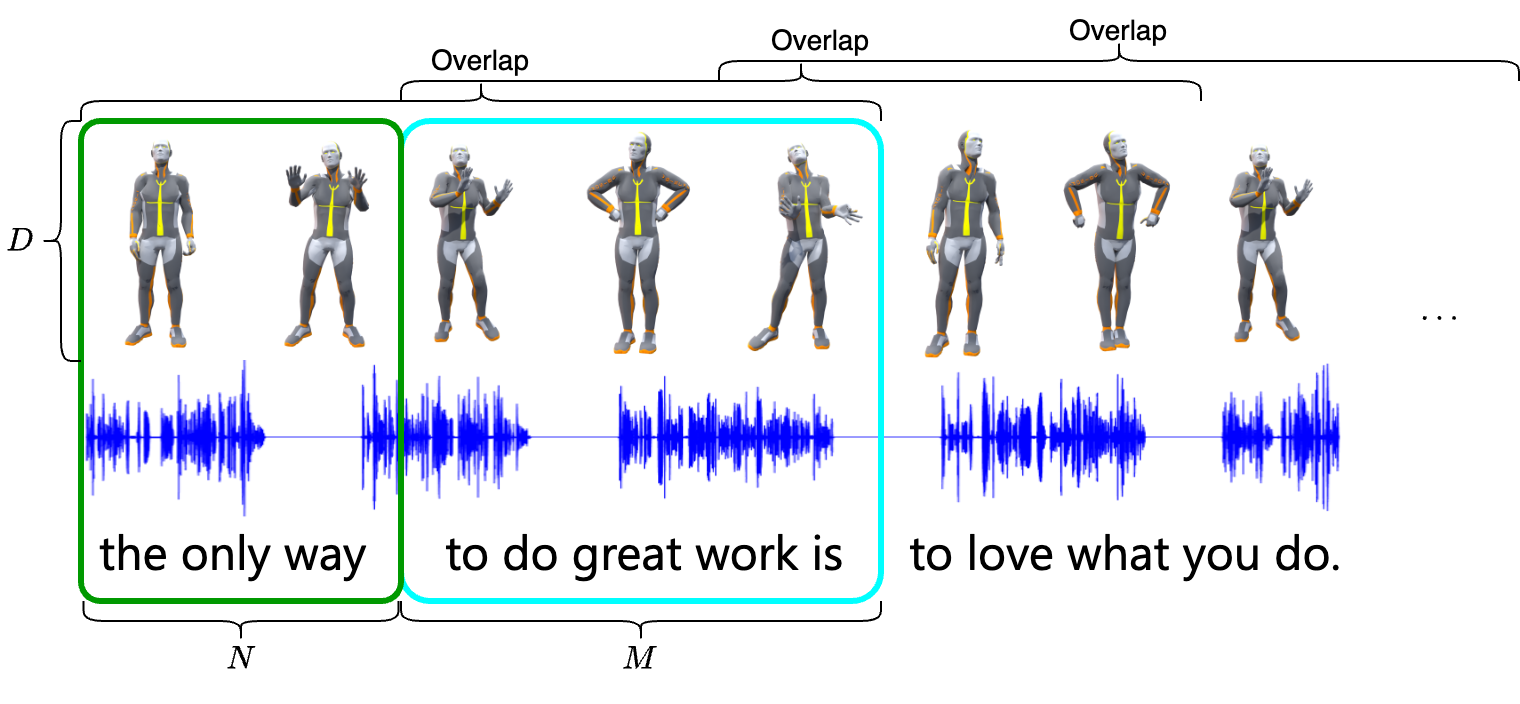
\includegraphics[width=\linewidth]{GestureSeries.jpg}
	\caption{Minh hoạ một chuỗi cử chỉ, ta lấy $N$ frame đầu làm cử chỉ khởi tạo $\mathbf{s}$ (seed gesture) và $M$ khung hình còn lại làm cử chỉ để học}
	\label{fig:GestureSeries}
\end{figure}


Quá trình xử lý dữ liệu được trình bày đầy đủ ở \autoref{appendix:BVHData}.


%Quá trình chuyển từ không gian Eule sang không gian Quaternion được minh hoạ ở phụ lục \ref{}
%Chuỗi waveform sẽ được cắt thành các đoạn chồng nhau, áp dụng Hamming windows, và áp dụng thuật toán fast fourier transform để biến đổi chuỗi giọng nói thành các hệ số thể hiện cường độ của các tần số trong chuỗi giọng nói, các hệ số này được làm tròn thành các đoạn tần số (frequency bins), các đoạn hệ số này được chuẩn hoá theo hệ cơ số log để tương ứng với cảm nhận của tai người để có được đặc trưng MFCC $\mathbf{a} \in \mathbb{R}^{\text{size} \times \mathcal{C}}$ trong đó $\mathcal{C}=13$ là số frequency bins. 


% \begin{figure}
%     \centering
%     \includegraphics[width=3cm]{images/gesture_sample.png}
%     \caption{Minh họa cử chỉ}
%     \label{fig:gesture_sample}
% \end{figure}

\section{Các khó khăn cần giải quyết}

Có rất nhiều khó khăn trong việc xây dựng một mô hình có thể học được các đặc trưng cử chỉ hội thoại như con người.

Thứ nhất, \textit{dữ liệu không đủ nhiều và chất lượng}, chi phí để tạo ra một bộ dữ liệu trong ngành công nghiệp chụp chuyển động có chất lượng và quy mô lớn để ứng dụng thực tế là rất cao.

Thứ hai, \textit{sự thiếu đồng nhất về ngữ cảnh của các loại dữ liệu}, các bộ dữ liệu về văn bản thường nhiều hơn so với giọng nói, và cũng không rõ văn bản đó được tạo ra bởi ai. Sự đồng bộ giữa giọng nói và cảm xúc khi nói cũng thường thiếu trong tập dữ liệu. Ngoài ra, dữ liệu văn bản trong tập dữ liệu huấn luyện lại thuộc nhiều chủ đề đa dạng.
 
Thứ ba, \textit{sự phân bố không cân xứng về  dữ liệu giữa các loại đăng trưng cần học}. Các dữ liệu dùng cho nghiên cứu cử chỉ hiện nay thường tập trung vào ngôn ngữ Tiếng Anh, các cử chỉ có sự phân bố không cân xứng giữa các trạng thái như nói, hỏi, hoặc im lặng.

Thứ tư, \textit{chi phí tính toán với nhiều loại dữ liệu của mô hình là một thách thức lớn}. Với đầu vào của mô hình gồm nhiều loại dữ liệu như văn bản, tiếng nói và điểm 3D, cần nhiều lớp mã hóa cho từng loại dữ liệu, dẫn đến chi phí tính toán cao trong cả giai đoạn huấn luyện và suy luận. Nếu giảm thông tin dữ liệu đầu vào cũng sẽ giảm kết quả suy luận của mô hình khi sinh cử chỉ.

Cuối cùng, \textit{các bước xử lý cần được thực hiện tuần tự}, cách hiệu quả nhất để con người tương tác với máy tính là thông qua giọng nói và nhập từ bàn phím, tuy nhiên việc xử lý được văn bản và giọng nói để làm đầu vào cho mô hình phải thực hiện tuần tự. Độ trễ trong quá trình suy luận của sản phẩm thực tế cũng là một vấn đề lớn, vì người dùng không thể chờ đợi quá lâu để nhận kết quả. Ngoài ra, việc hiển thị cử chỉ đó lên máy tính bằng kỹ thuật đồ họa cũng cần được tối ưu để giảm thời gian xử lý.


\section{Đóng góp dự kiến}

%	\item Tích hợp đặc trưng văn bản vào mô hình DiffuseStyleGesture:** Chúng tôi cải tiến DiffuseStyleGesture bằng cách đưa thông tin văn bản vào quá trình khử nhiễu có điều kiện, giúp hệ thống sinh ra các cử chỉ chi tiết và phù hợp hơn với nội dung hội thoại.

\begin{itemize}
	\item Dựa trên tập dữ liệu có sẵn, luận văn chuyển giọng nói trong tập dữ liệu thành văn bản, và dùng văn bản đó để làm dữ liệu huấn luyện mới như là một dữ liệu ngữ nghĩa bổ sung trong quá trình học.
	
	\item Dựa trên mô hình cơ bản DiffuseStyleGesture, luận văn mở rộng thêm đặc trưng văn bản trong quá trình khử nhiễu có điều kiện.
	
	\item Luận văn sử dụng Unity để render, trích xuất dữ liệu và trực quan hoá kết quả sinh cử chỉ.
	
	\item Luận văn xây dựng hệ thống kết xuất, và minh hoạ chương trình bằng Unity
\end{itemize}



%	với thông tin thời gian cho việc sinh cử chỉ kèm theo lời nói dựa trên giọng nói. Nhờ mô hình diffusion, luận văn có thể kiểm soát một cách linh hoạt cử chỉ được sinh ra, ví dụ: chỉnh sửa phong cách của cử chỉ, thiết lập cử chỉ khởi tạo, và sinh cử chỉ đa dạng.

%	\item Chúng tôi sử dụng cross-local attention và self-attention để để học được bối cảnh và những quan hệ giữa cử chỉ và lời nói.
%	
%	\item Các thử nghiệm mở rộng chỉ ra rằng mô hình của luận văn có thể sinh ra cử chỉ giống người, phù hợp với lời nói (speech-appropriateness), phù hợp với cảm xúc (style-appropriateness) vượt trội so với các phương pháp sinh cử chỉ hiện có.

%\item **Sử dụng Unity để render, trích xuất dữ liệu và trực quan hoá kết quả sinh cử chỉ:** Chúng tôi triển khai Unity như một công cụ trực quan hóa để mô phỏng và hiển thị kết quả của hệ thống sinh cử chỉ. Với các tính năng mô phỏng 3D mạnh mẽ, Unity cho phép luận văn kiểm nghiệm và đánh giá hiệu quả của các cử chỉ được sinh ra từ mô hình, đồng thời hỗ trợ trực quan hóa các đặc trưng chuyển động của cử chỉ. Hệ thống cũng sẽ được phát triển để cho phép dễ dàng trích xuất dữ liệu cử chỉ và so sánh kết quả trực quan giữa các mô hình khác nhau, giúp nâng cao tính khả thi và giá trị thực nghiệm của hệ thống.
%
%\item **Xây dựng hệ thống kết xuất và minh hoạ chương trình bằng Unity:** Ngoài việc render và trực quan hóa kết quả sinh cử chỉ, luận văn phát triển hệ thống kết xuất hoàn chỉnh, bao gồm các thành phần giúp dễ dàng minh hoạ quá trình sinh cử chỉ theo từng giai đoạn. Hệ thống này không chỉ cung cấp công cụ để kiểm nghiệm chất lượng cử chỉ sinh mà còn giúp mô tả rõ ràng từng bước trong quá trình sinh cử chỉ, từ giai đoạn tiền xử lý dữ liệu, khử nhiễu, đến việc ứng dụng các đặc trưng văn bản và giọng nói để tạo ra cử chỉ. Điều này sẽ làm tăng tính minh bạch và khả năng giải thích của hệ thống, đồng thời hỗ trợ các nhà nghiên cứu và người dùng dễ dàng quan sát và hiểu sâu hơn về các bước sinh cử chỉ. 



% Ngôn ngữ để viết và trình bày báo cáo khóa luận tốt nghiệp, đồ án tốt nghiệp, thực tập tốt nghiệp (sau đây gọi chung là báo cáo) là tiếng Việt hoặc tiếng Anh. 
% Trường hợp chọn ngôn ngữ tiếng Anh để viết và trình bày báo cáo,  sinh viên cần có đơn đề nghị, được cán bộ hướng dẫn (CBHD) đồng ý và nộp cho bộ phận Giáo vụ của Khoa vào thời điểm đăng ký đề tài để xin ý kiến.
% Báo cáo viết và trình bày bằng tiếng Anh phải có bản tóm tắt viết bằng tiếng Việt.


%Tóm tắt luận văn được trình bày nhiều nhất trong 24 trang in trên hai mặt giấy, cỡ chữ Times New Roman 11 của hệ soạn thảo Winword hoặc phần mềm soạn thảo Latex đối với các chuyên ngành thuộc ngành Toán.

%Mật độ chữ bình thường, không được nén hoặc kéo dãn khoảng cách giữa các chữ.
%Chế độ dãn dòng là Exactly 17pt.
%Lề trên, lề dưới, lề trái, lề phải đều là 1.5 cm.
%Các bảng biểu trình bày theo chiều ngang khổ giấy thì đầu bảng là lề trái của trang.
%Tóm tắt luận án phải phản ảnh trung thực kết cấu, bố cục và nội dung của luận án, phải ghi đầy đủ toàn văn kết luận của luận án.
%Mẫu trình bày trang bìa của tóm tắt luận văn (phụ lục 1).


\chapter{TỔNG QUAN}
\label{Chapter2}

Bài toán sinh cử chỉ cũng tương tự như các bài toán khác đều đã nghiên cứu và phát triển song hành với các phương pháp học máy truyền thống và hiện đại. Gồm các nhóm phương pháp dựa trên luật và các phương pháp dựa trên dữ liệu.  Đầu tiên luận văn chứng minh mối quan hệ giữa cử chỉ và giọng nói \autoref{sec:relationspeechandgesture}, từ đó là tiền đề thể hiện sự đồng bộ về dữ liệu giữa cử chỉ và giọng nói và việc học mối quan hệ giữa cử chỉ và giọng nói có ý nghĩa. Trong mục \autoref{sec:commonstage} Luận văn sẽ trình bày về các công đoạn chung trong các phương pháp sinh cử chỉ.
Ở phần \autoref{sec:relatedwork} luận văn trình bày về các phương pháp đã được sử dụng trong quá trình sinh cử chỉ. Luận văn sẽ so sánh các phương pháp, từ đó nêu lý do luận văn sử dụng mô hình diffusion để áp dụng cho bài toán sinh cử chỉ.
Trong phần \autoref{sec:diffusionbase}, luận văn sẽ trình bày về cách các mô hình diffusion được áp dụng cho bài toán sinh cử chỉ gần đây.

\section{Mối quan hệ giữa cử chỉ và giọng nói}
\label{sec:relationspeechandgesture}

Theo ngôn ngữ học, cử chỉ có thể được phân thành 6 nhóm chính: cử chỉ thích nghi (adaptors), cử chỉ biểu tượng (emblems), cử chỉ chỉ định (deictics), cử chỉ biểu trưng (iconics), cử chỉ ẩn dụ (metaphorics), và cử chỉ nhấn mạnh (beat) \cite{ekman1969repertoire}, \cite{sebeok2011advances}. Trong số đó, cử chỉ nhấn mạnh không mang ý nghĩa ngữ nghĩa trực tiếp nhưng đóng vai trò quan trọng trong việc đồng bộ nhịp điệu giữa giọng nói và cử chỉ \cite{kipp2005gesture}, \cite{sebeok2011advances}. Tuy nhiên, nhịp điệu giữa giọng nói và cử chỉ nhấn mạnh không hoàn toàn đồng bộ, khiến việc học mối quan hệ thời gian giữa chúng trở nên phức tạp \cite{mcclave1994gestural}, \cite{bhattacharya2021speech2affectivegestures}, \cite{kucherenko2020gesticulator}, \cite{yoon2020speech}.

Cử chỉ tương tác với các cấp độ thông tin khác nhau trong giọng nói \cite{sebeok2011advances}. Chẳng hạn, cử chỉ biểu tượng, như hành động giơ ngón cái, thường liên quan đến thông tin ngữ nghĩa cấp cao (ví dụ: "tốt" hoặc "tuyệt vời"), trong khi cử chỉ nhấn mạnh thường đi kèm với thông tin cấp thấp như nhấn mạnh trong âm thanh. Các nghiên cứu trước đây thường chỉ sử dụng đặc trưng từ lớp cuối cùng của bộ mã hóa giọng nói để tổng hợp cử chỉ \cite{alexanderson2020style}, \cite{bhattacharya2021speech2affectivegestures}, \cite{kucherenko2021large}, \cite{qian2021speech}, \cite{yoon2022genea}. Tuy nhiên, cách tiếp cận này có thể làm trộn lẫn thông tin từ nhiều cấp độ, dẫn đến khó khăn trong việc phân tách rõ ràng nhịp điệu và ngữ nghĩa.

Như các nghiên cứu ngôn ngữ học chỉ ra \cite{kipp2005gesture}, \cite{neff2008gesture}, \cite{webb1997linguistic}, cử chỉ trong giao tiếp hàng ngày có thể được chia thành một số lượng giới hạn các đơn vị ngữ nghĩa với các biến thể chuyển động khác nhau. Dựa trên giả định này, được phân tách đặc trưng giọng nói thành hai loại: đặc trưng cấp cao đại diện cho các đơn vị ngữ nghĩa, và đặc trưng cấp thấp xác định các biến thể chuyển động. Từ đó, mối liên hệ giữa chúng được học thông qua các lớp khác nhau của bộ mã hóa giọng nói. Các thử nghiệm chứng minh rằng cơ chế này có khả năng tách biệt rõ ràng các đặc trưng ở nhiều cấp độ, đồng thời tổng hợp được cử chỉ phù hợp về ngữ nghĩa và phong cách.


\section{Các công đoạn chung trong bài toán sinh cử chỉ}
\label{sec:commonstage}

Cách tiếp cận với bài toán sinh cử chỉ (gesture generation) được thực hiện với nhiều phương pháp khác nhau. Tuy nhiên luận văn tổng quát hoá lại thành các công đoạn chính như \autoref{fig:CommonStage} sau:

\begin{figure}[H]
	\centering
	\includegraphics[width=\textwidth]{CommonStage}
	\caption{Các công đoạn trong mô hình sinh cử chỉ cử chỉ.}
	\label{fig:CommonStage}
\end{figure}

Như đã trình bày ở \autoref{sec:ProblemStatement}, cử chỉ bao gồm chuỗi chuyển động của toạ độ điểm 3D bao gồm 

\begin{enumerate}[label=\textbf{\arabic*.}]
	\item \textbf{Tiền xử lý dữ liệu}: 
	
	\item \textbf{Xử lý đặc trưng}: 
	
	\item \textbf{Trích xuất đặc trưng}
	
	\item \textbf{Mã hoá đặc trưng}
	
	\item \textbf{Kết hợp đặc trưng}
	
	\item \textbf{Giải mã đặc trưng}
	
	\item \textbf{Kết xuất}
\end{enumerate}

\section{Tổng quan các phương pháp cho bài toán sinh cử chỉ}
\label{sec:relatedwork}



\subsection{Phương pháp dựa trên luật}

Các phương pháp dựa trên luật thường ánh xạ (mappings) từng giọng nói với từng đơn vị cử chỉ \cite{huang2012robot}. Và luật được tạo thủ công. Phương pháp dựa trên luật thì chúng ta có thể dễ dàng điều khiển kết quả của mô hình và có khả năng giải thích tốt kết quả dự đoán của mô hình.
Tuy nhiên chi phí để tạo thủ công là không khả thi để xây dựng cho các ứng dụng phức tạp đòi hỏi phải xử lý một lượng dữ liệu rất lớn.

\subsection{Phương pháp dựa trên thống kê}

Tương tự như phương pháp dựa trên luật, phương pháp dựa trên dữ liệu cũng ánh xạ các đặc trưng của giọng nói tương ứng với cử chỉ nhưng thay vì làm thủ công thì được sử dụng học một cách tự động dựa trên dữ liệu.
Trong đó có hai phương pháp chính là phương pháp thống kê và phương pháp dựa trên dữ liệu.

%\subsubsection{Phương pháp thống kê}

Phương pháp thống kê sử dụng phân phối xác suất để tìm sự tương đồng giữa các đặc trưng giọng nói và cử chỉ \cite{levine2010gesture}. Tác giả \cite{neff2008gesture} xây dựng mô hình để học từng phong cách của từng người nói.

\subsection{Phương pháp học sâu}

\setcounter{figure}{3}
\begin{figure}[H]
	\centering
	\includegraphics[width=0.8\textwidth]{GeneralOverview}
	\caption{Tổng quan về các mô hình tạo sinh khác nhau.}
	\label{fig:GeneralOverview}
\end{figure}

Phương pháp sinh cử chỉ được chia thành hai nhóm chính. Bao gồm các mô hình ước lượng log likelihood (likelihood-based model)  và phương pháp dựa vào các mô hình sinh ngầm định (implicit generative models) \cite{song2021score}. 

\subsubsection{Likelihood-based Model}

Phương pháp học ước lượng log likelihood là phương pháp học trực tiếp từ hàm mật độ xác xuất (probability density) thông qua maximum likelihood. Các phương pháp điển hình là autoregressive models, normalizing flow models, energy-based models (EBMs)
, và variational auto-encoders (VAEs).

%Phương pháp học sâu sử dụng mạng nơ-ron (neural) thông qua nhiều lớp ẩn để học một cách tự động các phối xác xuất giữa cử chỉ và giọng nói.

Mô hình được kết hợp với văn bản đầu vào được gắn thẻ với chủ đề, trọng tâm câu và thành ngữ để tạo ra các kịch bản cử chỉ, sau đó được ánh xạ sang một chuỗi các cử chỉ được chọn từ một từ điển hoạt họa. \cite{chiu2015predicting} huấn luyện một model classifier neural network để chọn một đơn vị cử chỉ phù hợp dựa trên đầu vào là giọng nói. 
%Nghiên cứu gần đây đã bắt đầu tận dụng học sâu và huấn luyện các mô hình kết thúc đến cuối sử dụng dữ liệu cử chỉ thô trực tiếp, giải phóng các nỗ lực thủ công trong thiết kế từ điển cử chỉ và các quy tắc ánh xạ.

Cử chỉ có thể được tổng hợp bằng các mô hình xác định như perceptron đa tầng (MLP) \cite{kucherenko2020gesticulator}, recurrent neural networks \cite{bhattacharya2021speech2affectivegestures}, \cite{liu2022learning}, \cite{hasegawa2018evaluation}, \cite{yoon2020speech}, convolutional networks \cite{habibie2021learning} và transformer \cite{bhattacharya2021text2gestures} 

\subsubsection{Implicit Generative Models}

Trong các phương pháp dựa vào mô hình sinh ngầm định, phân phối của dữ liệu được học một cách ngầm định thông qua việc quá trình lấy mẫu (sampling). Ví dụ tiêu biểu nhất là mô hình generative adversarial networks (GANs). Khi dữ liệu được tổng hợp bằng cách chuyển phân phối dữ liệu ban đầu ở dạng phân phối chuẩn về phân phối của dữ liệu.

%
%\begin{table}[h!]
%	\small
%	\centering
%	\renewcommand{\arraystretch}{1.5} % Tăng khoảng cách giữa các hàng
%	\begin{tabular}{|p{0.2\textwidth}|p{0.35\textwidth}|p{0.35\textwidth}|}
%		\hline
%		\textbf{Loại phương pháp} & \textbf{Ưu điểm} & \textbf{Nhược điểm} \\ \hline
%		Rule-Based  & 
%		- Dễ hiểu và dễ triển khai. \newline 
%		- Dễ giải thích và có thể kiểm soát được \newline
%		- Hiệu quả trong các trường hợp đơn giản hoặc dữ liệu nhỏ. & 
%		- Không tổng quát hoá tốt với dữ liệu phức tạp. \newline 
%		- Đòi hỏi nhiều công sức trong việc xây dựng quy tắc thủ công. \\ \hline
%		Likelihood-Based Models & 
%		- Khả năng ước lượng mật độ xác suất của dữ liệu \newline 
%		- Có khả năng mở rộng và học từ dữ liệu lớn & 
%		- Dễ bị ảnh hưởng bởi nhiễu \newline 
%		- Kết quả thấp ở vùng dữ liệu hiếm \newline
%		- Khả năng sinh không đa dạng \\ \hline
%		Implicit Generative Models & 
%		- Tạo ra dữ liệu chất lượng cao. \newline 
%		- Linh hoạt và đa dạng \newline
%		- Phủ được vùng có mật độ dữ liệu thấp & 
%		- Cần cấu hình phức tạp để đạt hiệu năng tốt. \newline 
%		- Khó đánh giá do mỗi lần nhiễu là khác nhau. \newline 
%		- Quá trình lấy mẫu chậm \\ \hline
%	\end{tabular}
%	\caption{Bảng so sánh ưu và nhược điểm của các phương pháp}
%\end{table}

\begin{table}[h!]
	\small
	\centering
	\renewcommand{\arraystretch}{1.5} % Tăng khoảng cách giữa các hàng
	\resizebox{\textwidth}{!}{ % Giảm kích thước bảng để vừa với trang
		\begin{tabular}{|p{0.2\textwidth}|p{0.35\textwidth}|p{0.35\textwidth}|p{0.2\textwidth}|}
			\hline
			\textbf{Phương pháp tiêu biểu} & \textbf{Ưu điểm} & \textbf{Nhược điểm} & \textbf{Loại phương pháp} \\ \hline
			Robot behavior toolkit \cite{huang2012robot} & 
			- Dễ hiểu và dễ triển khai. \newline 
			- Dễ giải thích và có thể kiểm soát được \newline
			- Hiệu quả trong các trường hợp đơn giản hoặc dữ liệu nhỏ. & 
			- Không tổng quát hoá tốt với dữ liệu phức tạp. \newline 
			- Đòi hỏi nhiều công sức trong việc xây dựng quy tắc thủ công. & 
			Rule-Based  \\ \hline
			MLP \cite{kucherenko2020gesticulator}, RNN \cite{bhattacharya2021speech2affectivegestures}, \cite{liu2022learning}, \cite{hasegawa2018evaluation}, \cite{yoon2020speech}, CNN \cite{habibie2021learning}, Transformer \cite{bhattacharya2021text2gestures}  & 
			- Khả năng ước lượng mật độ xác suất của dữ liệu \newline 
			- Có khả năng mở rộng và học từ dữ liệu lớn & 
			- Dễ bị ảnh hưởng bởi nhiễu \newline 
			- Kết quả thấp ở vùng dữ liệu hiếm \newline
			- Khả năng sinh không đa dạng & 
			Likelihood-Based Models \\ \hline
			\textbf{DiffusionStyle-Gesture} \cite{yang2022DiffuseStyleGestureplus}, MDM \cite{tevet2022human}, Motiondiffuse \cite{zhang2022motiondiffuse} &
			- Tạo ra dữ liệu chất lượng cao. \newline 
			- Linh hoạt và đa dạng \newline
			- Phủ được vùng có mật độ dữ liệu thấp & 
			- Cần cấu hình phức tạp để đạt hiệu năng tốt. \newline 
			- Khó đánh giá do mỗi lần nhiễu là khác nhau. \newline 
			- Quá trình lấy mẫu chậm & 
			Implicit Generative Models \\ \hline
		\end{tabular}
	}
	\caption{Bảng so sánh ưu và nhược điểm của các phương pháp}
\end{table}

%Trong mục tiêu theo luận văn sẽ trình bày các phương pháp sử dụng mô hình Diffusion.

%chuyển phân phối của dữ liệu ở dạng phân phối chuẩn hay ở một vị trí bất kỳ về phân phối chuẩn bằng hàm neuron network. 


%WGAN \cite{wu2021probabilistic}.



%\textbf{Bảng so sánh các phương pháp}
%
%\begin{table}[ht]
%	\centering
%	\begin{tabular}{|l|l|l|l|l|l|}
%		\hline
%		\textbf{Phương pháp} & \textbf{Loại mô hình} & \textbf{Đặc điểm nổi bật} & \textbf{Ưu điểm} & \textbf{Hạn chế} & \textbf{Tài liệu tham khảo} \\ \hline
%		VAE  & Autoencoder & Biểu diễn dữ liệu trong không gian tiềm ẩn & Tạo đặc trưng ẩn & Khó kiểm soát đầu ra & \cite{kingma2013auto} \\ \hline
%		VQ-VAE & Autoencoder (cải tiến) & Dùng codebook cho không gian tiềm ẩn & Biểu diễn chi tiết hơn & Phức tạp hơn & \cite{van2017neural} \\ \hline
%		RNN & Mạng hồi tiếp & Xử lý chuỗi dữ liệu & Tốt cho dữ liệu tuần tự & Khó huấn luyện & \cite{bhattacharya2021speech2affectivegestures} \\ \hline
%		Transformer & Mạng chú ý & Tạo cử chỉ qua cơ chế chú ý & Hiệu quả với dữ liệu dài & Yêu cầu nhiều tài nguyên & \cite{bhattacharya2021text2gestures} \\ \hline
%		WGAN & GAN & Học phân phối dữ liệu đối kháng & Tạo sự đa dạng & Khó huấn luyện & \cite{wu2021probabilistic} \\ \hline
%		Normalizing Flow & Mô hình xác suất & Học phân phối phức tạp & Hữu ích với dữ liệu phức tạp & Cần tài nguyên tính toán lớn & \cite{alexanderson2020style} \\ \hline
%		Diffusion Models & Mô hình sinh dữ liệu & Chi tiết cao, xử lý dữ liệu thiếu & Tạo cử chỉ chi tiết & Thời gian huấn luyện lâu & \cite{xu2022freeform} \\ \hline
%	\end{tabular}
%	\caption{So sánh các phương pháp sinh cử chỉ}
%\end{table}

%


\section{Công đoạn chung của phương pháp học sâu trong bài toán sinh cử chỉ}
\label{sec:commonstage}

Như đã trình bày ở \autoref{sec:Data}, cử chỉ bao gồm chuỗi chuyển động của toạ độ điểm 3D. Với mỗi tập dữ liệu số lượng xương (bone) mỗi khung hình sẽ khác nhau. 

Cách tiếp cận bằng học sâu với bài toán sinh cử chỉ (gesture generation) được thực hiện với nhiều phương pháp khác nhau. Tuy nhiên luận văn tổng quát hoá lại thành các công đoạn chính như \autoref{fig:CommonStage} sau:

\begin{figure}[H]
	\centering
	\includegraphics[width=\textwidth]{CommonStage}
	\caption{Các công đoạn trong mô hình sinh cử chỉ cử chỉ.}
	\label{fig:CommonStage}
\end{figure}

\begin{enumerate}[label=\textbf{\arabic*.}]
	\item \textbf{Tiền xử lý dữ liệu}: Trong công đoạn tiền xử lý, các dữ liệu về giọng nói ở dạng định wav, tệp BVH và văn bản sẽ được đọc, số hoá để thu được các vector hoặc ma trận thể hiện thông tin thô của dữ liệu. Đối với mỗi phương pháp học khác nhau, các thông tin dữ liệu ban đầu sẽ được chọn để học cũng khác nhau.
	
	\item \textbf{Xử lý đặc trưng}: Trong công đoạn xử lý đặc trưng, các dữ liệu thô như giọng nói và văn bản được nhúng (embedding) để biểu diễn thành các vector đặc trưng. Các phương pháp khác nhau sẽ chọn các mô hình nhúng khác nhau. Việc biểu diễn các cử chỉ của nhân vật thành các vector đặc trưng của mỗi phương pháp cũng khác nhau.
	
	\item \textbf{Trích xuất đặc trưng}: Công đoạn trích xuất đặc trưng sẽ dùng các lớp biến đổi tuyến tính (linear) hoặc các lớp CNN để trích xuất các đặc trưng của dữ liệu. Các dữ liệu về văn bản hoặc giọng nói sau khi xử lý đặc trưng có thể cũng được cho đi qua các lớp trích xuất đặc trưng để biểu diễn thành các vector đặc trưng để biểu diễn tương ứng với văn bản và giọng nói.
	
	\item \textbf{Mã hoá đặc trưng}: Trong công đoạn mã hoá đặc trưng, các vector về cử chỉ, cảm xúc, và giọng nói sẽ được biểu diễn lên không gian tiềm ẩn nhỏ hơn kích thước ban đầu nhằm thuận tiện cho việc tính sự tương quan giữa các đặc trưng ở công đoạn kết hợp đặc trưng.
	
	\item \textbf{Kết hợp đặc trưng}: Trong công đoạn kết hợp đặc trưng, các đặc trưng giọng nói, văn bản, cử chỉ cũng như các thông tin khác được kết hợp với nhau bằng việc concat, các lớp kết nối đầy đủ hoặc kết hợp các đặc trưng bằng cách cộng hoặc trừ các vector tiềm ẩn.
	
	\item \textbf{Giải mã đặc trưng}: Trong công đoạn giải mã đặc trưng, các đặc vector tiềm ẩn sẽ được giải mã hay tăng chiều dữ liệu về kích thước ban đầu.
	
	\item \textbf{Kết xuất} (Render): Sau khi có được vector ở kích thước ban đầu, các vector sẽ được biến đổi ngược trở về các tệp BVH để kết xuất bằng các phần mềm như Blender hoặc Unity để minh học các chuyển động của nhân vật.
\end{enumerate}



\section{Diffusion-base Model}
\label{sec:diffusionbase}



Với đặc điểm dữ liệu là giá trị của các góc quay, các toạ độ của điểm khớp, nên cần độ chi tiết cao để tạo ra sự chân thực trong các chuyển động của nhân vật. Ngoài ra dữ liệu sẽ thiếu và rất ít dữ liệu trong các trường hợp cực trị của tham số.
Nên luận văn sử dụng mô hình Diffusion, với đặc điểm là có thể học được độ chi tiết cao hơn và có thể phủ được dữ liệu trong các trường hợp cực trị của tham số và độ phủ về mật độ dữ liệu thấp.



%❖ Chương này tập trung trình bày chi tiết những gì bạn
%làm
%❖ Mô tả chi tiết phương pháp thực hiện, giải pháp đề xuất, ứng dụng phát triển
%❖ Có thể đưa ra ví dụ minh họa để dẫn nhập
%❖ Nên phân thành các mục con
%   
%❖ Hướng nghiên cứu: Phương pháp đề xuất (Proposed Approach)
%o Cơ sở lý thuyết
%o Câu hỏi nghiên cứu, giả thuyết khoa học
%o Phương pháp/Thủ tục thực hiện nghiên cứu (procedure)
%o Đối tượng nghiên cứu
%o Môi trường (phần mềm, thư viện, máy móc, công cụ, v.v...)
%o Mô tả dữ liệu, quá trình thu thập dữ liệu
%o Độ đo để đánh giá (performance metrics)

%\chapter{PHƯƠNG PHÁP ĐỀ XUẤT}
\chapter{PHƯƠNG PHÁP NGHIÊN CỨU}
\label{Chapter3}

%\begin{figure}
%    \centering
%    \includegraphics[width=\linewidth]{images/architecture.jpg}
%    \caption{Kiến trúc mồ hình sinh cử chỉ OHGesture}
%    \label{fig:architecture}
%\end{figure}

Bản chất của các phương pháp dựa trên neuron network là ước lượng xác xuất của dữ liệu (probability density) nên cần chuẩn hoá (normalization), trong khi mô hình Diffusion sẽ học để có thể ước lượng đạo hàm của phân phối dữ liệu (estimating gradients of data distribution) và không phải chuẩn hoá trên toàn bộ dữ liệu \cite{song2021score}, nên có kết quả tốt hơn so với các phương pháp neuron network không sử dụng diffusion.
Mô hình diffusion có khả năng mô phỏng phân phối dữ liệu trong các trường hợp mật độ phân phối của dữ liệu thấp và có thể sinh được kết quả với độ chi tiết cao nên phù hợp với bài toán sinh cử chỉ. Mô hình của luận văn dựa trên mô hình DiffuseStyleGesture \cite{yang2022DiffuseStyleGestureplus} với cải tiến để có thể học theo cảm xúc của nhân vật. Trước tiên luận văn trình bày về mô hình diffusion \autoref{sec:summary_diffusion}, và phần \autoref{sec:ohgesture} sẽ trình bày về mô hình đề xuất OHGesture. 

%Diffusion \cite{ho2020denoising} là mô hình được lấy cảm hứng từ mô hình khuếch tán các chất trong hóa học.

\section{Mô hình diffusion cơ bản}
\label{sec:summary_diffusion}

\setcounter{figure}{4}
\begin{figure}[H]
	\centering
	\includegraphics[width=\linewidth]{DiffuseAndDenoise}
	\caption{Minh hoạ quá trình gây nhiễu (Diffuse) và khử nhiễu (Denoise) cử chỉ chưa qua quá trình huấn luyện}
	\label{fig:DiffuseAndDenoise}
\end{figure}

Với các phương pháp sử dụng neural network như ResNet, GAN,... mục tiêu là tìm được trọng số $\theta$ của hàm $f_{\theta}(x)$, Hàm mà đầu vào là $x$, chúng ta sẽ cực tiểu hoá hàm lỗi $\mathcal{L}_\text{loss}$ giữa nhãn $y$ và kết quả dự đoán là $\hat{y}$. Sau khi kết thúc quá trình huấn luyện và học được trọng số $\theta'$ ta dự đoán một mẫu dữ liệu mới $x'$ bằng cách forward qua hàm $f_{\theta'}$ để ra được kết quả dự đoán $y'$.

%\begin{figure*}[bp]


Tương tự phương pháp VAE, mã hoá (encode) ma trận đầu vào thành vector tiềm ẩn $z$ và giải mã (decode) vector tiềm ẩn $z$ ngược trở lại ma trận kích thước ban đầu, tuy nhiên mô hình diffusion chia quá trình học thành từng $T$ bước, ở bước thứ $t$ quá trình gây nhiễu (forward diffusion process) $q(\mathbf{x})$ từ $1 \to T$ được thực hiện bằng cách thêm nhiễu $\epsilon \sim \mathcal{N} (\mathbf{0}, \mathbf{I})$ phân phối chuẩn Gaussian vào dữ liệu, với giá trị trung bình  (mean) bằng $\mathbb{E}[\epsilon]=0$ và độ lệch chuẩn $\operatorname{Var}(\epsilon)=1$, $\mathbf{I}$ là phần tử đơn vị của phân phối chuẩn Gaussian. Trong \autoref{fig:DiffuseAndDenoise} quá trình giảm nhiễu từ trái qua phải, còn quá trình khử nhiễu từ phải qua trái $p_\theta(x)$. Trong quá trình khử nhiễu (denoising process) từ $T \to 1$, mục tiêu là học được trọng số $\theta$ của hàm dữ đoán nhiễu $f_{\theta}$ hay còn được ký hiệu là hàm dự đoán lượng nhiễu ($\epsilon_\theta$) đã được thêm vào. Sau khi kết thúc quá trình học và ta có trọng số $\theta'$ của hàm dự đoán nhiễu $\hat{\epsilon}$ , ta sẽ dùng hàm $f_{\theta'}$ để dự đoán nhiễu. Sau khi có nhiễu dự đoán $\hat{\epsilon}$, chúng ta trừ đi ảnh bị nhiễu $\mathbf{x}_{t}$ để có được ảnh khử nhiễu $\mathbf{x}_{t-1}$, và cộng với nhiễu $ \mathbf{z} \in \mathcal{N}(0, \mathbf{I})$ để tạo ra sự đa dạng cử chỉ. Thực hiện lần lượt từ $T \to 1$ để có được ảnh dự đoán $\hat{\bx_0}$. Như \autoref{fig:basic_diffusion} là kiến trúc đầy đủ của mô hình diffusion tiêu chuẩn (Denoising Diffusion Probabilistic Models - DDPM).

\subsection{Quá trình gây nhiễu (forward diffusion process)}

Cho dữ liệu $\mathbf{x}_{0}$ là được lấy từ dữ liệu thật $\mathbf{x}_{0} \sim q(x)$, với mỗi bước ta sẽ thêm nhiễu vào đầu vào $\bx_{0}$ với tỷ lệ nhiễu và ảnh gốc được kiểm soát bằng hệ số $\beta$:
\vspace{-20pt}
\setcounter{figure}{5}
\begin{figure*}[H]
	\centering
	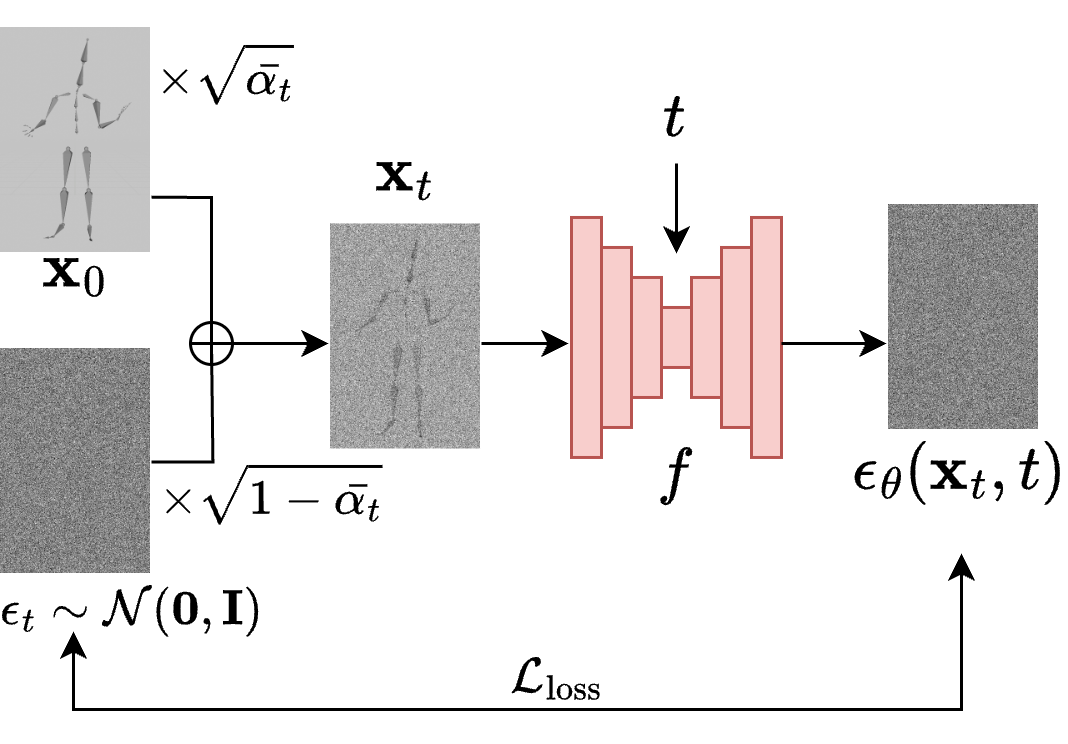
\includegraphics[height=180pt]{AlgorithmForwardDiffusion}
	\vspace{-5pt}
	\caption{Minh hoạ quá trình huấn luyện và làm nhiễu (Diffuse)}
	\label{fig:AlgorithmForwardDiffusion}
	\vspace{-10pt}
\end{figure*}


\begin{equation}
	\label{eq:addgaussian}
	\mathbf{x}_t = \sqrt{1 - \beta_t}\mathbf{x}_{t-1} + \sqrt{\beta_t} \boldsymbol{\epsilon}_{t-1}
\end{equation}

Trong đó, quá trình gây nhiễu từ $1 \to T$, với mỗi bước $t$ quá trình thêm nhiễu $\epsilon$ được điều khiển bằng $\beta_t$ theo phương sai $\{\beta_t \in (0, 1)\}_{t=1}^T$:

\begin{equation}
	\label{eq:forward_diffusion_process}
	\begin{aligned}
		q(\mathbf{x}_t \vert \mathbf{x}_{t-1}) &= \mathcal{N}(\mathbf{x}_t; \sqrt{1 - \beta_t} \mathbf{x}_{t-1}, \beta_t\mathbf{I}) \quad \\
		q(\mathbf{x}_{1:T} \vert \mathbf{x}_0) &= \prod^T_{t=1} q(\mathbf{x}_t \vert \mathbf{x}_{t-1})
	\end{aligned}
\end{equation}

Mục tiêu ở bước $t$ của hệ số $\sqrt{1 - \beta_t}$ và $\beta_t$ là để lần lượt giảm tỷ lệ của ảnh gốc $x_t$ và tăng dần nhiễu  $\boldsymbol{\epsilon}_{t-1}$, vì vậy $\beta_1 < \beta_2 < \dots < \beta_T$. Khi $T \to \infty$ thì $x_{T}$ sẽ hoàn toàn nhiễu \cite{weng2021diffusion} (Isotropic Gaussian Distribution) $q(T) = \mathcal{N} (0, \mathbf{I})$.


Vì nhiễu $\boldsymbol{\epsilon}_{t-1}, \boldsymbol{\epsilon}_{t-2}, \dots \sim \mathcal{N}(\mathbf{0}, \mathbf{I})$ luôn luôn là phân phối chuẩn Gaussian, và cho trước trong mọi bước $t$, nên ta có thể dễ dàng truy ngược được $\bx_t$ từ $\bx_0$. Bằng cách đặt $\alpha_t = 1 - \beta_t$ và $\bar{\alpha}_t = \prod_{i=1}^t \alpha_i$, từ \autoref{eq:addgaussian}, ta có hàm forward diffusion viết lại theo $\alpha$ như sau:

%\begin{equation}
%%	\label{eq:tracexzero}
%	\begin{aligned}
%		\mathbf{x}_t 
%		&= \sqrt{\alpha_t}\mathbf{x}_{t-1} + \sqrt{1 - \alpha_t}\boldsymbol{\epsilon}_{t-1} \\
%		&= \sqrt{\alpha_t \alpha_{t-1}} \mathbf{x}_{t-2} + \sqrt{1 - \alpha_t \alpha_{t-1}} \bar{\boldsymbol{\epsilon}}_{t-2}
%		&= \sqrt{\bar{\alpha}_t}\mathbf{x}_0 + \sqrt{1 - \bar{\alpha}_t}\boldsymbol{\epsilon} \\
%		q(\mathbf{x}_t \vert \mathbf{x}_0) &= \mathcal{N}(\mathbf{x}_t; \sqrt{\bar{\alpha}_t} \mathbf{x}_0, (1 - \bar{\alpha}_t)\mathbf{I})
%	\end{aligned}
%\end{equation}

\begin{equation}
\begin{aligned}
	\boldsymbol{x}_t &= \sqrt{\alpha_t}\boldsymbol{x}_{t-1} + \sqrt{1 - \alpha_t}\boldsymbol{\epsilon}_{t-1} \\
	&= \sqrt{\alpha_t}\left(\sqrt{\alpha_{t-1}}\boldsymbol{x}_{t-2} + \sqrt{1 - \alpha_{t-1}}\boldsymbol{\epsilon}_{t-2}\right) + \sqrt{1 - \alpha_t}\boldsymbol{\epsilon}_{t-1} \\
	&= \sqrt{\alpha_t\alpha_{t-1}}\boldsymbol{x}_{t-2} + \sqrt{\alpha_t(1 - \alpha_{t-1})}\boldsymbol{\epsilon}_{t-2} + \sqrt{1 - \alpha_t}\boldsymbol{\epsilon}_{t-1} \\
	&= \sqrt{\alpha_t\alpha_{t-1}}\boldsymbol{x}_{t-2} + \sqrt{\alpha_t(1 - \alpha_{t-1}) + (1 - \alpha_t)}\boldsymbol{\epsilon}_{t-2} \\
	&= \sqrt{\alpha_t\alpha_{t-1}}\boldsymbol{x}_{t-2} + \sqrt{1 - \alpha_t\alpha_{t-1}}\boldsymbol{\epsilon}_{t-2} \\
	&= \ldots \\
	&= \sqrt{\prod_{i=1}^t \alpha_i} \boldsymbol{x}_0 + \sqrt{1 - \prod_{i=1}^t \alpha_i} \boldsymbol{\epsilon}_0 \\
	&= \sqrt{\bar{\alpha}_t} \boldsymbol{x}_0 + \sqrt{1 - \bar{\alpha}_t} \boldsymbol{\epsilon}_0 \\
	&\sim \mathcal{N}\left(\boldsymbol{x}_t; \sqrt{\bar{\alpha}_t} \boldsymbol{x}_0, \left(1 - \bar{\alpha}_t\right) \textbf{I}\right)
\end{aligned}
\label{eq:tracexzero}
\end{equation}

Sự thay đổi của $\sqrt{\alpha}$ và  $\sqrt{1- \alpha}$ trong quá trình gây nhiễu được thể hiện ở phụ lục \autoref{Appendix2}

\subsection{Quá trình khử nhiễu (denoising process)}
\label{subsection:denoising_process}

\setcounter{figure}{6}
\begin{figure}[H]
	\centering
	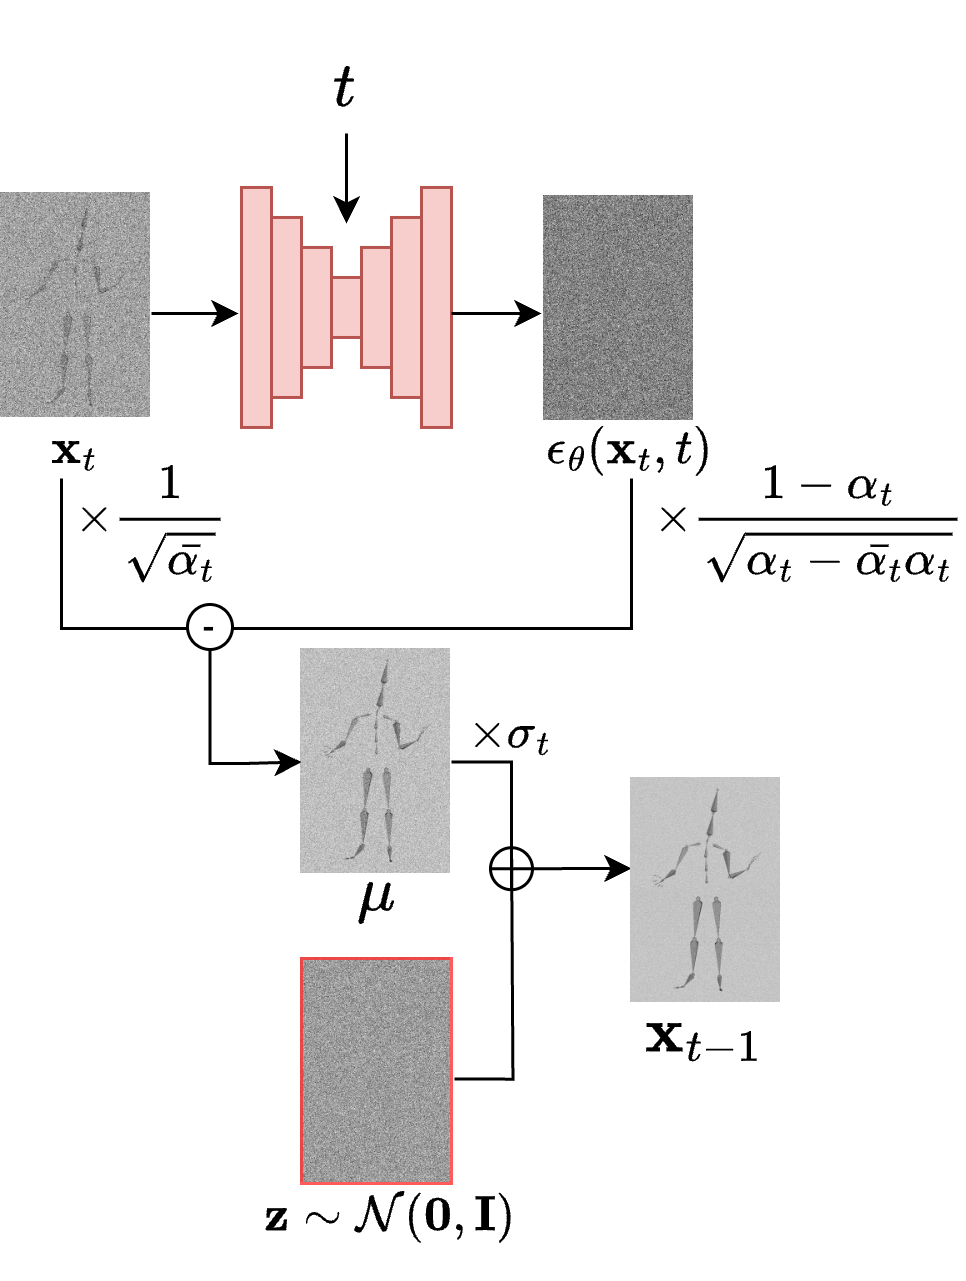
\includegraphics[height=280pt]{AlgorithmSamplingDiffusion}
	\caption{Minh hoạ quá trình khử nhiễu (Denoise)}
	\label{fig:AlgorithmSamplingDiffusion}
	\vspace{-5pt}
\end{figure}

Quá trình khử nhiễu $p_\theta(\mathbf{x}_{t-1} \vert \mathbf{x}_t)$  ở bước thứ $t$ từ $T \to 1$ được bắt đầu từ $\bx_T$ là hoàn toàn nhiễu $\mathcal{N} (\mathbf{0}, \mathbf{I})$. Ta sẽ dùng một neural network $f_{\theta} (x_t, t)$ để dự đoán nhiễu $\hat{\epsilon} = f_{\theta}(\bx_t, t)$ đã được thêm vào để được $\bx_{t-1}$ từ $\bx_t$.

Quá trình khử nhiễu có trung bình $\boldsymbol{\mu}_\theta(\mathbf{x}_t, t) = {\frac{1}{\sqrt{\alpha_t}} \Big( \mathbf{x}_t - \frac{1 - \alpha_t}{\sqrt{1 - \bar{\alpha}_t}}  f_\theta(\mathbf{x}_t, t) \Big)}$ và độ lệch chuẩn $\boldsymbol{\Sigma}_\theta(\mathbf{x}_t, t)$ như sau:


%\begin{equation} \mathrm{d}\mathbf{x} = [\mathbf{f}(\mathbf{x}, t) - g^2(t) \nabla_\mathbf{x} \log p_t(\mathbf{x})]\mathrm{d}t + g(t) \mathrm{d} \mathbf{w}.\label{rsde} \end{equation}

% bằng cách lấy ảnh bị nhiễu trừ đi nhiễu dự đoán

\begin{equation}
	\label{eq:denoising_process}
	\begin{aligned}
		p_\theta(\mathbf{x}_{0:T})
		&= p(\mathbf{x}_T) \prod^T_{t=1} p_\theta(\mathbf{x}_{t-1} \vert \mathbf{x}_t) \\
		p_\theta(\mathbf{x}_{t-1} \vert \mathbf{x}_t) &= \mathcal{N}(\mathbf{x}_{t-1};  \boldsymbol{\mu}_\theta(\mathbf{x}_t, t), \boldsymbol{\Sigma}_\theta(\mathbf{x}_t, t))
	\end{aligned}
\end{equation}

Qúa trình khử nhiễu là quá trình bắt đầu từ nhiễu hoàn toàn, dùng một neuron network $f_\theta$ để học được quá trình khử nhiễu.

%Ta viết lại hàm denoising từ công thức \ref{eq:denoising_process}  theo $\alpha$ như sau:
%$$
%x_{t-1} = \frac{1}{\sqrt{\alpha_t}} \left( x_t - \frac{\sqrt{1 - \alpha_t}}{\sqrt{1 - \bar{\alpha}_t}} \epsilon_{\theta}(x_t, t) \right) + \sqrt{1 - \alpha_t} \tilde{\epsilon}_t
%$$


%\begin{equation}
%	\label{eq:denoising_alpha}
%	\begin{aligned}
	%	p_\theta(\mathbf{x}_{t-1} \vert \mathbf{x}_t) &= \mathcal{N}(\mathbf{x}_{t-1}; \boldsymbol{\mu}_\theta(\mathbf{x}_t, t), \boldsymbol{\Sigma}_\theta(\mathbf{x}_t, t))
	%\end{aligned} \\
	% \bar{\boldsymbol{\mu}}_t (x_t, t) = \frac{1}{\sqrt{\alpha_t}} \Big( \mathbf{x}_t - \frac{1 - \alpha_t}{\sqrt{1 - \bar{\alpha}_t}} \boldsymbol{\epsilon}_t \Big)
	%\end{equation}
%\subsection{Hàm mất mát trong }


\subsection{Quá trình huấn luyện trong mô hình diffusion cơ bản}
%	Hàm mất mát $\mathcal{L}$ của mô hình diffusion
	
	\begin{figure}[H]
		\centering
		\includegraphics[width=\linewidth]{DDPMTraining}
		\caption{Mô hình diffusion cơ bản}
		\label{fig:basic_diffusion}\
		\vspace{-5pt}
	\end{figure}
	
	Mô hình diffusion sẽ học trọng số $\theta$ của hàm dự đoán lỗi $f_{\theta} (x_t, t)$ hay còn ký hiệu là  $\epsilon_{\theta} (x_t, t)$. Trong quá trình denoising, ta sẽ tối ưu độ lỗi giữa nhiễu dự đoán $\boldsymbol{\epsilon}_\theta(\mathbf{x}_t, t)$ và nhiễu thực tế $\boldsymbol{\epsilon}_t$. Với mỗi bước thứ $t$ ta sẽ tối ưu hàm loss $\mathcal{L}_{t}$ để thu được trọng số $\theta$.
	
	\begin{equation}
		\label{eq:diffusion_loss}
		\begin{aligned}
			\mathcal{L}_t
			&= \mathbb{E}_{t \sim [1, T], \mathbf{x}_0, \boldsymbol{\epsilon}_t} \Big[\|\boldsymbol{\epsilon}_t - \boldsymbol{\epsilon}_\theta(\mathbf{x}_t, t)\|^2 \Big] \\
			&= \mathbb{E}_{t \sim [1, T], \mathbf{x}_0, \boldsymbol{\epsilon}_t} \Big[\|\boldsymbol{\epsilon}_t - \boldsymbol{\epsilon}_\theta(\sqrt{\bar{\alpha}_t}\mathbf{x}_0 + \sqrt{1 - \bar{\alpha}_t}\boldsymbol{\epsilon}_t, t)\|^2 \Big]
		\end{aligned}
	\end{equation}
	
	
Với $f_{\theta}(x_{t-1}, t)$ hay $\epsilon_\theta$ là một mô hình Unet dùng để mã hoá và giải mã dữ liệu để dự đoán nhiễu đã thêm vào dữ liệu. Quá trình tính toán hàm lỗi được trình bày minh hoạ trong \autoref{fig:basic_diffusion}.


\begin{algorithm}[H]
	\caption{Thuật toán training trong DDPM}
	\setlength{\baselineskip}{10pt}
	\begin{enumerate}
		\vspace{5pt}
		\item Tính sẵn các giá trị $\sqrt{\alpha_t}$, $\sqrt{1 - \alpha_t}$ và $\sqrt{\bar{\alpha}_t}$ cho mỗi bước $t: 1 \rightarrow T$. Xác định lịch trình nhiễu $\{\alpha_t \in (0, 1)\}_{t=1}^T$, với $\alpha_1 < \alpha_2 < \dots < \alpha_T$.
		
		\item Lấy nhãn $\mathbf{x}_0$ từ phân phối của dữ liệu đã chuẩn hoá.
		
		\item Tạo nhiễu ngẫu nhiên $\boldsymbol{\epsilon}_t$ cho mỗi bước $t: 1 \rightarrow T$, với $\forall t: \boldsymbol{\epsilon}_t \sim \mathcal{N}(\mathbf{0}, \mathbf{I})$.
		
		\item Gây nhiễu (forward) $\mathbf{x}_0$ để thu được $\mathbf{x}_t$ ở mỗi bước $t: 1 \rightarrow T$:
		$$
		\mathbf{x}_t = \sqrt{\bar{\alpha}_t} \mathbf{x}_0 + \sqrt{1 - \bar{\alpha}_t} \boldsymbol{\epsilon}_t
		$$
		
		\item Với mỗi $t$, lấy $t$ \textbf{ngẫu nhiên} từ $[1, T]$.
		
		\item Cho $\mathbf{x}_t$ và $t$ vào mô hình để dự đoán nhiễu: $\hat{\boldsymbol{\epsilon}} = \boldsymbol{\epsilon}_\theta(\mathbf{x}_t, t)$.
		
		\item Tính đạo hàm để cập nhật trọng số:
		$$
		\grad_{\theta_t} \left\| \boldsymbol{\epsilon}_t - \boldsymbol{\epsilon}_\theta(\mathbf{x}_t, t) \right\|^2
		$$
		Tính loss:
		$$
		\mathcal{L}_t = \mathbb{E}_{t \sim [1, T], \mathbf{x}_0, \boldsymbol{\epsilon}_t} \left[ \|\boldsymbol{\epsilon}_t - \boldsymbol{\epsilon}_\theta(\sqrt{\bar{\alpha}_t} \mathbf{x}_0 + \sqrt{1 - \bar{\alpha}_t} \boldsymbol{\epsilon}_t, t)\|^2 \right]
		$$
		
		\item Quay lại bước 6 cho đến khi hội tụ để thu được trọng số tối ưu $\theta'$.
	\end{enumerate}
\end{algorithm}

%	Lưu ý 
%	Thay vì dùng neuron network để dự đoán phân bố của dữ liệu theo như hình \ref{fig:basic_diffusion}, mô hình diffusion sẽ dự đoán độ lỗi được thêm vào trong ảnh ở bước thứ $t$, với mỗi $t$ bước ta sẽ cần tối ưu hàm mất mát $\mathcal{L}_t$, hàm mất mát của mỗi bước sẽ tối ưu độ lỗi giữa nhiễu dự đoán $\hat{\epsilon_t}$ và nhiễu nhãn $\epsilon_t$ được thêm vào.
	
\subsection{Quá trình lấy mẫu trong diffusion cơ bản}
	
		\begin{figure*}
		\centering
		\includegraphics[width=\linewidth]{GaussianDrift.jpg}
		\caption{Quá trình Training và Sampling trong mô hình Diffusion tiêu chuẩn}
		\label{fig:GaussianDrift}
	\end{figure*}
	

	Sau khi thu được trọng số $\theta'$, ta sẽ dùng hàm denoising để khử nhiễu từ nhiễu $\bx_T \sim \mathcal{N} (\mathbf{0}, \mathbf{I})$.
	Quá trình biến đổi từ nhiễu hoàn toàn $\bx_{T}$ sang dự đoán $\hat{\bx_0}$ như sau:
	%với $t$ là một vector đã được nhúng vị trí bằng thuật toán nhúng
	
	\begin{equation}
		\label{eq:adddenoising}
	\bx_{t-1} = \frac{1}{\sqrt{\alpha_t}} \left( \bx_t - \frac{1- \alpha_t}{\sqrt{1 - \bar{\alpha}_t}} f_{\theta'}(\bx_t, t) \right) + \sqrt{1 - \alpha_t} \tilde{\epsilon}_t
	\end{equation}
	
Lưu ý rằng $\epsilon_t$ là nhiễu cố định và lấy ngẫu nhiên trước quá trình huấn luyện, chỉ sử dụng lại kết quả ngẫu nhiên trong quá trình forward diffusion \autoref{subsection:denoising_process} ở công thức  \autoref{eq:addgaussian}. Như \autoref{fig:GaussianDrift}, độ lỗi $\epsilon_t$ là độ nhiễu của từng bước $t$, và hàm loss  $\mathcal{L}^{t}$ sẽ tính theo từng bước $t$.


Tiếp theo quá trình huấn luyện, thuật toán lấy mẫu (sampling) trong DDPM bắt đầu từ bước tạo nhiễu hoàn toàn, tức là $\mathbf{x}_T \sim \mathcal{N}(0, \mathbf{I})$, nơi dữ liệu ban đầu hoàn toàn là nhiễu. Các giá trị $\sqrt{\alpha_t}$, $\sqrt{1 - \alpha_t}$ và $\sqrt{\bar{\alpha}_t}$, được tính từ quá trình huấn luyện, sẽ được sử dụng trong quá trình lấy mẫu để dự đoán lại dữ liệu gốc $\mathbf{x}_0$. Bước tiếp theo là tính toán hệ số điều chỉnh nhiễu $\sigma_t$, dựa vào lịch trình nhiễu $\alpha_t$ đã xác định trong quá trình huấn luyện. Các giá trị này sẽ ảnh hưởng đến độ nhiễu được thêm vào trong quá trình lấy mẫu ngược.

Thuật toán lấy mẫu sẽ được thực hiện từ bước $T$ trở về $1$, và trong mỗi bước, một nhiễu ngẫu nhiên $\mathbf{z} \sim \mathcal{N}(0, \mathbf{I})$ được tạo ra để cộng thêm vào kết quả dự đoán. Tại mỗi bước $t$, mô hình sẽ dự đoán nhiễu $\boldsymbol{\epsilon}_{\theta'}$ dựa trên dữ liệu nhiễu $\mathbf{x}_t$ và bước thời gian $t$, sau đó sử dụng dự đoán này để tính toán giá trị $\mu$, là ước lượng của $\mathbf{x}_0$. Cuối cùng, một lượng nhiễu $\sigma_t \mathbf{z}$ được cộng thêm vào $\mu$ để thu được $\hat{\mathbf{x}}{t-1}$, dữ liệu nhiễu tại bước $t-1$. Quá trình này tiếp tục cho đến khi $t = 1$, và khi đó, chúng ta có được $\hat{\mathbf{x}}_0$ — dự đoán cuối cùng của dữ liệu gốc từ quá trình khử nhiễu.

%Mục tiêu của quá trình lấy mẫu này là phục hồi lại dữ liệu ban đầu $\mathbf{x}_0$ từ nhiễu hoàn toàn, đồng thời đảm bảo tính ổn định và sự đa dạng trong quá trình sinh mẫu thông qua việc sử dụng nhiễu ngẫu nhiên $\mathbf{z}$.


\begin{algorithm}[H]
	\caption{Thuật toán sampling trong DDPM}
	\label{alg:samplingddpm}
	\setlength{\baselineskip}{10pt}
	\begin{enumerate}
		\item Bắt đầu với nhiễu: $\mathbf{x}_T \sim \mathcal{N}(0, \mathbf{I})$.
		
		\item Các giá trị $\sqrt{\alpha_t}$, $\sqrt{1 - \alpha_t}$ và $\sqrt{\bar{\alpha}_t}$ được lấy từ quá trình huấn luyện.
		
		\item Tính hệ số điều chỉnh nhiễu $\sigma_t$ từ $\alpha_t$ ở mỗi bước $t: 1 \rightarrow T$:
		\[
		\sigma_t = \sqrt{\frac{1 - \bar{\alpha}_{t-1}}{1 - \bar{\alpha}_t} (1 - \alpha_t)}
		\]
		
		\item Với mỗi $t$, lấy $t$ \textbf{tuần tự} từ $[T, \dots, 1]$.
		
		\item Tạo nhiễu ngẫu nhiên $\mathbf{z} \sim \mathcal{N}(0, \mathbf{I})$.
		
		\item Đưa $\mathbf{x}_t$ vào mô hình để suy luận nhiễu: $\boldsymbol{\epsilon}_{\theta'} = \boldsymbol{\epsilon}_{\theta'}(\mathbf{x}_t, t)$.
		
		\item Dùng nhiễu dự đoán để trừ đi $\mathbf{x}_t$ ở bước $t$:
		\[
		\mu = \frac{1}{\sqrt{\alpha_t}} \left( \mathbf{x}_t - \frac{1 - \alpha_t}{\sqrt{1 - \bar{\alpha}_t}} \boldsymbol{\epsilon}_{\theta'}(\mathbf{x}_t, t) \right)
		\]
		
		\item Cộng thêm một lượng nhiễu: $\hat{\mathbf{x}}_{t-1} = \mu + \sigma_t \mathbf{z}$.
		
		\item Khi $t = 1$, thu được $\hat{\mathbf{x}}_0$ từ quá trình khử nhiễu.
	\end{enumerate}

\end{algorithm}

Điều quan trọng nhất trong quá trình lấy mẫu (denoising sampling) đó chính là phải cộng thêm một độ nhiễu $\mathbf{z} \in \mathcal{N}(0, \mathbf{I})$, với $\mathbf{z}$  sẽ được lần lượt thêm ở từng bước $t$ bằng hệ số điều khiển $\sigma_t$. Mục tiêu của nhiễu $\epsilon$ là để  làm gờ phân phối (marginal noise distribution) cho mô hình $f_\theta$ (hay $\epsilon_{\theta}$) có thể học được nhiễu, còn với  $\mathbf{z}$ là để tăng tính đa dạng trong quá trình sinh và sự ổn định trong quá trình lấy mẫu. Thuật toán lấy mẫu được trình bày ở \autoref{alg:samplingddpm}.

% \section*{Mô hình sinh cử chỉ OHGesture}

% \section*{3 Phương Pháp Của Chúng Tôi}
% Diffusion là mô hình đằng sau các thành công của  Stable Diffusion, Midjourney và DALL-E trong việc tạo ra các tấm ảnh siêu thực.


%. Biếm tiềm ẩm ở đây là cử chỉ và điều kiện là cảm xúc. 
%Kiến trúc của OHGesture được trình bày như hình \autoref{fig:diffusion_forward}.
\pagebreak

\section{Mô hình của đề xuất OHGesture}
\label{sec:ohgesture}

%\begin{figure}
%	\centering
%	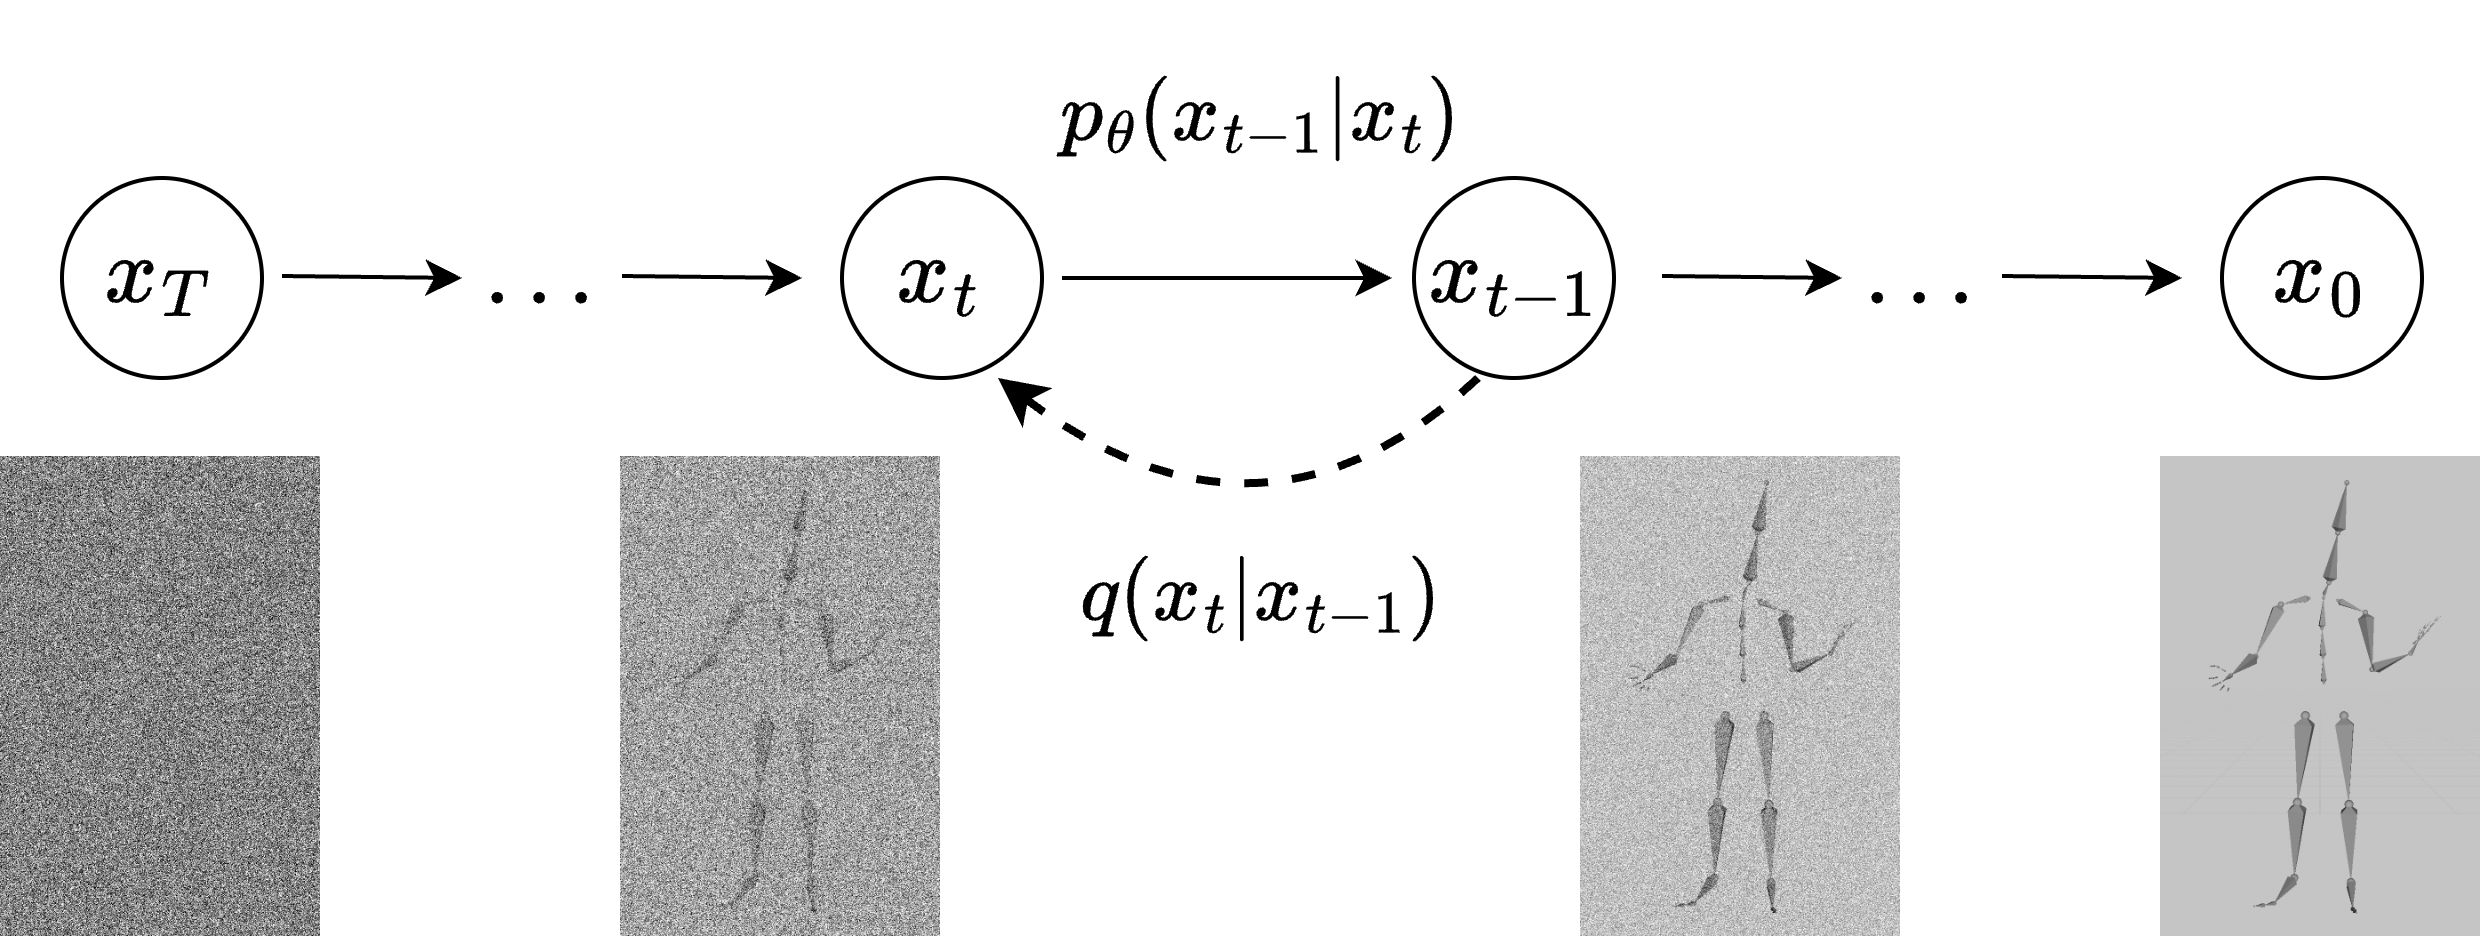
\includegraphics[width=\linewidth]{images/diffusion_forward}
%	\caption{Minh hoạ quá trình khử nhiễu (denoising) cử chỉ}
%	\label{fig:diffusion_forward}
%\end{figure}

%\begin{figure*}
%	\centering
%	\includegraphics[width=0.8\linewidth]{TrainingAndSampling}
%	\caption{Quá trình Huấn luyện và lấy mẫu trong OHGesture}
%%	\label{fig:TrainingAndSampling}
%\end{figure*}

\begin{figure}[H]
	\centering
	\includegraphics[width=\linewidth]{AllStage}
	\caption{Quá trình Huấn luyện và lấy mẫu trong OHGesture}
	\label{fig:TrainingAndSampling}
\end{figure}

Mô hình đề xuất \textbf{OHGesture} của chúng tôi được dựa trên mô hình \textbf{DiffuseStyleGesture} \cite{yang2023diffusestylegesture} áp dụng mô hình Diffusion \cite{ho2020denoising} có điều kiện \cite{ho2022classifier} (Classifier-Free Diffusion Guidance) để điều khiển các đặc trưng trong quá trình khử nhiễu. 
Không giống như trong mô hình DiffuseStyleGesture, chúng tôi sử dụng thêm điều kiện văn bản được nhúng bằng mô hình Pretrain FastText  \cite{bojanowski2017enriching}.

Những điểm giống và khác của việc áp dụng mô hình Diffusion cho bài toán sinh cử chỉ so với mô hình Diffusion trong bài toán sinh ảnh:

\vspace{10pt}

\textbf{Điểm giống}
\begin{itemize}
	\item Chúng tôi sử dụng mô hình Diffusion \cite{yang2023diffusestylegesture} trên cử chỉ $\bx^{1:M \times D}$,  với $M$ frame theo thời gian, $D=1141$ là các điểm toạ độ chuyển động của mỗi khung hình (tương tự width và height trong ảnh).
	\item Classifier-Free Diffusion Guidance với $\bx_0$ objective.
	\item Latent vector có số chiều là $256$.
\end{itemize}

\textbf{Điểm khác}

\begin{itemize}
	\item Sinh cử chỉ có điều kiện:
	\begin{itemize}
		\item Điều kiện cảm xúc: $c = \big[ \mathbf{s}, \mathbf{e}, \mathbf{a}, \mathbf{v} \big]$ và $c_{\varnothing} = \big[ \varnothing, \varnothing, \mathbf{a}, \mathbf{v}\big]$.
		\item Nội suy trạng thái giữa hai cảm xúc $\mathbf{e}_1, \mathbf{e}_2$, sử dụng điều kiện: $c = \big[ \mathbf{s}, \mathbf{e}_1, \mathbf{a}, \mathbf{v} \big]$ và $c_{\varnothing} = \big[ \mathbf{s}, \mathbf{e}_2, \mathbf{a}, \mathbf{v} \big]$.
	\end{itemize}
	\item Self-Attention: Mối liên hệ giữa các cảm xúc, cử chỉ khởi tạo và từng frame (tương tự DALL-E 2 - mối liên hệ giữa văn bản và ảnh).
	\item Concat âm thanh và văn bản (Giống ControlNet - Pixel-wise Condition)
	%			\item Học mối liên hệ giữa điều kiện và các frame bằng Local-Cross Attention
\end{itemize}

Trong đó $\bx_0$ là chuỗi $M$ khung hình cử chỉ $\mathbf{x} \in \mathbb{R}^{1:M \times D}$ ($D = 1141$), với điều kiện $c = [\mathbf{s}, \mathbf{e}, \mathbf{a}, \mathbf{v}]$ bao gồm cử chỉ khởi tạo (seed gesture) $\mathbf{s}$,  cảm xúc (emotion) $\mathbf{e}$, chuỗi âm thanh (audio) $\mathbf{a}$ tương ứng cử chỉ, và văn bản  $\mathbf{v}$.
%} \in \mathbb{R}^{M \times 300} 
%, chuỗi âm thanh thô $64000$ là $4$ giây với mỗi giây được đọc với sample rate là $16000$.

%Với đầu vào bao gồm cử chỉ khởi tạo $x_{\text{seed}}$, âm thanh $a$ và văn bản $t$.
% với biến tiềm ẩn   (diffusion latent variable)
Tương tự mô hình diffusion cơ bản bao gồm hai quá trình: quá trình tạo nhiễu (diffusion) $q$ và quá trình khử nhiễu (denoising process) $p_{\theta}$ với trọng số $\theta$. Quá trình Training và Sampling của mô hình đề xuất \textbf{OHGesture} được minh hoạ ở hình \ref{fig:TrainingAndSampling}.

\subsection{Quá trình trích xuất đặc trưng}

Dữ liệu để học của chúng tôi được lấy từ tập dữ liệu ZeroEGGS \cite{ghorbani2022zeroeggszeroshotexamplebasedgesture}. Bao gồm âm thanh, cử chỉ khởi tạo, cảm xúc và văn bản.
%Tương tự mô hình DiffuseStyleGesture \cite{yang2022DiffuseStyleGestureplus} chúng tôi cũng sử dụng đầu vào bao gồm âm thanh, cử chỉ và cảm xúc
%ngoài ra chúng tôi sử dụng thêm dữ liệu văn bản.
\begin{figure}[H]
	\centering
	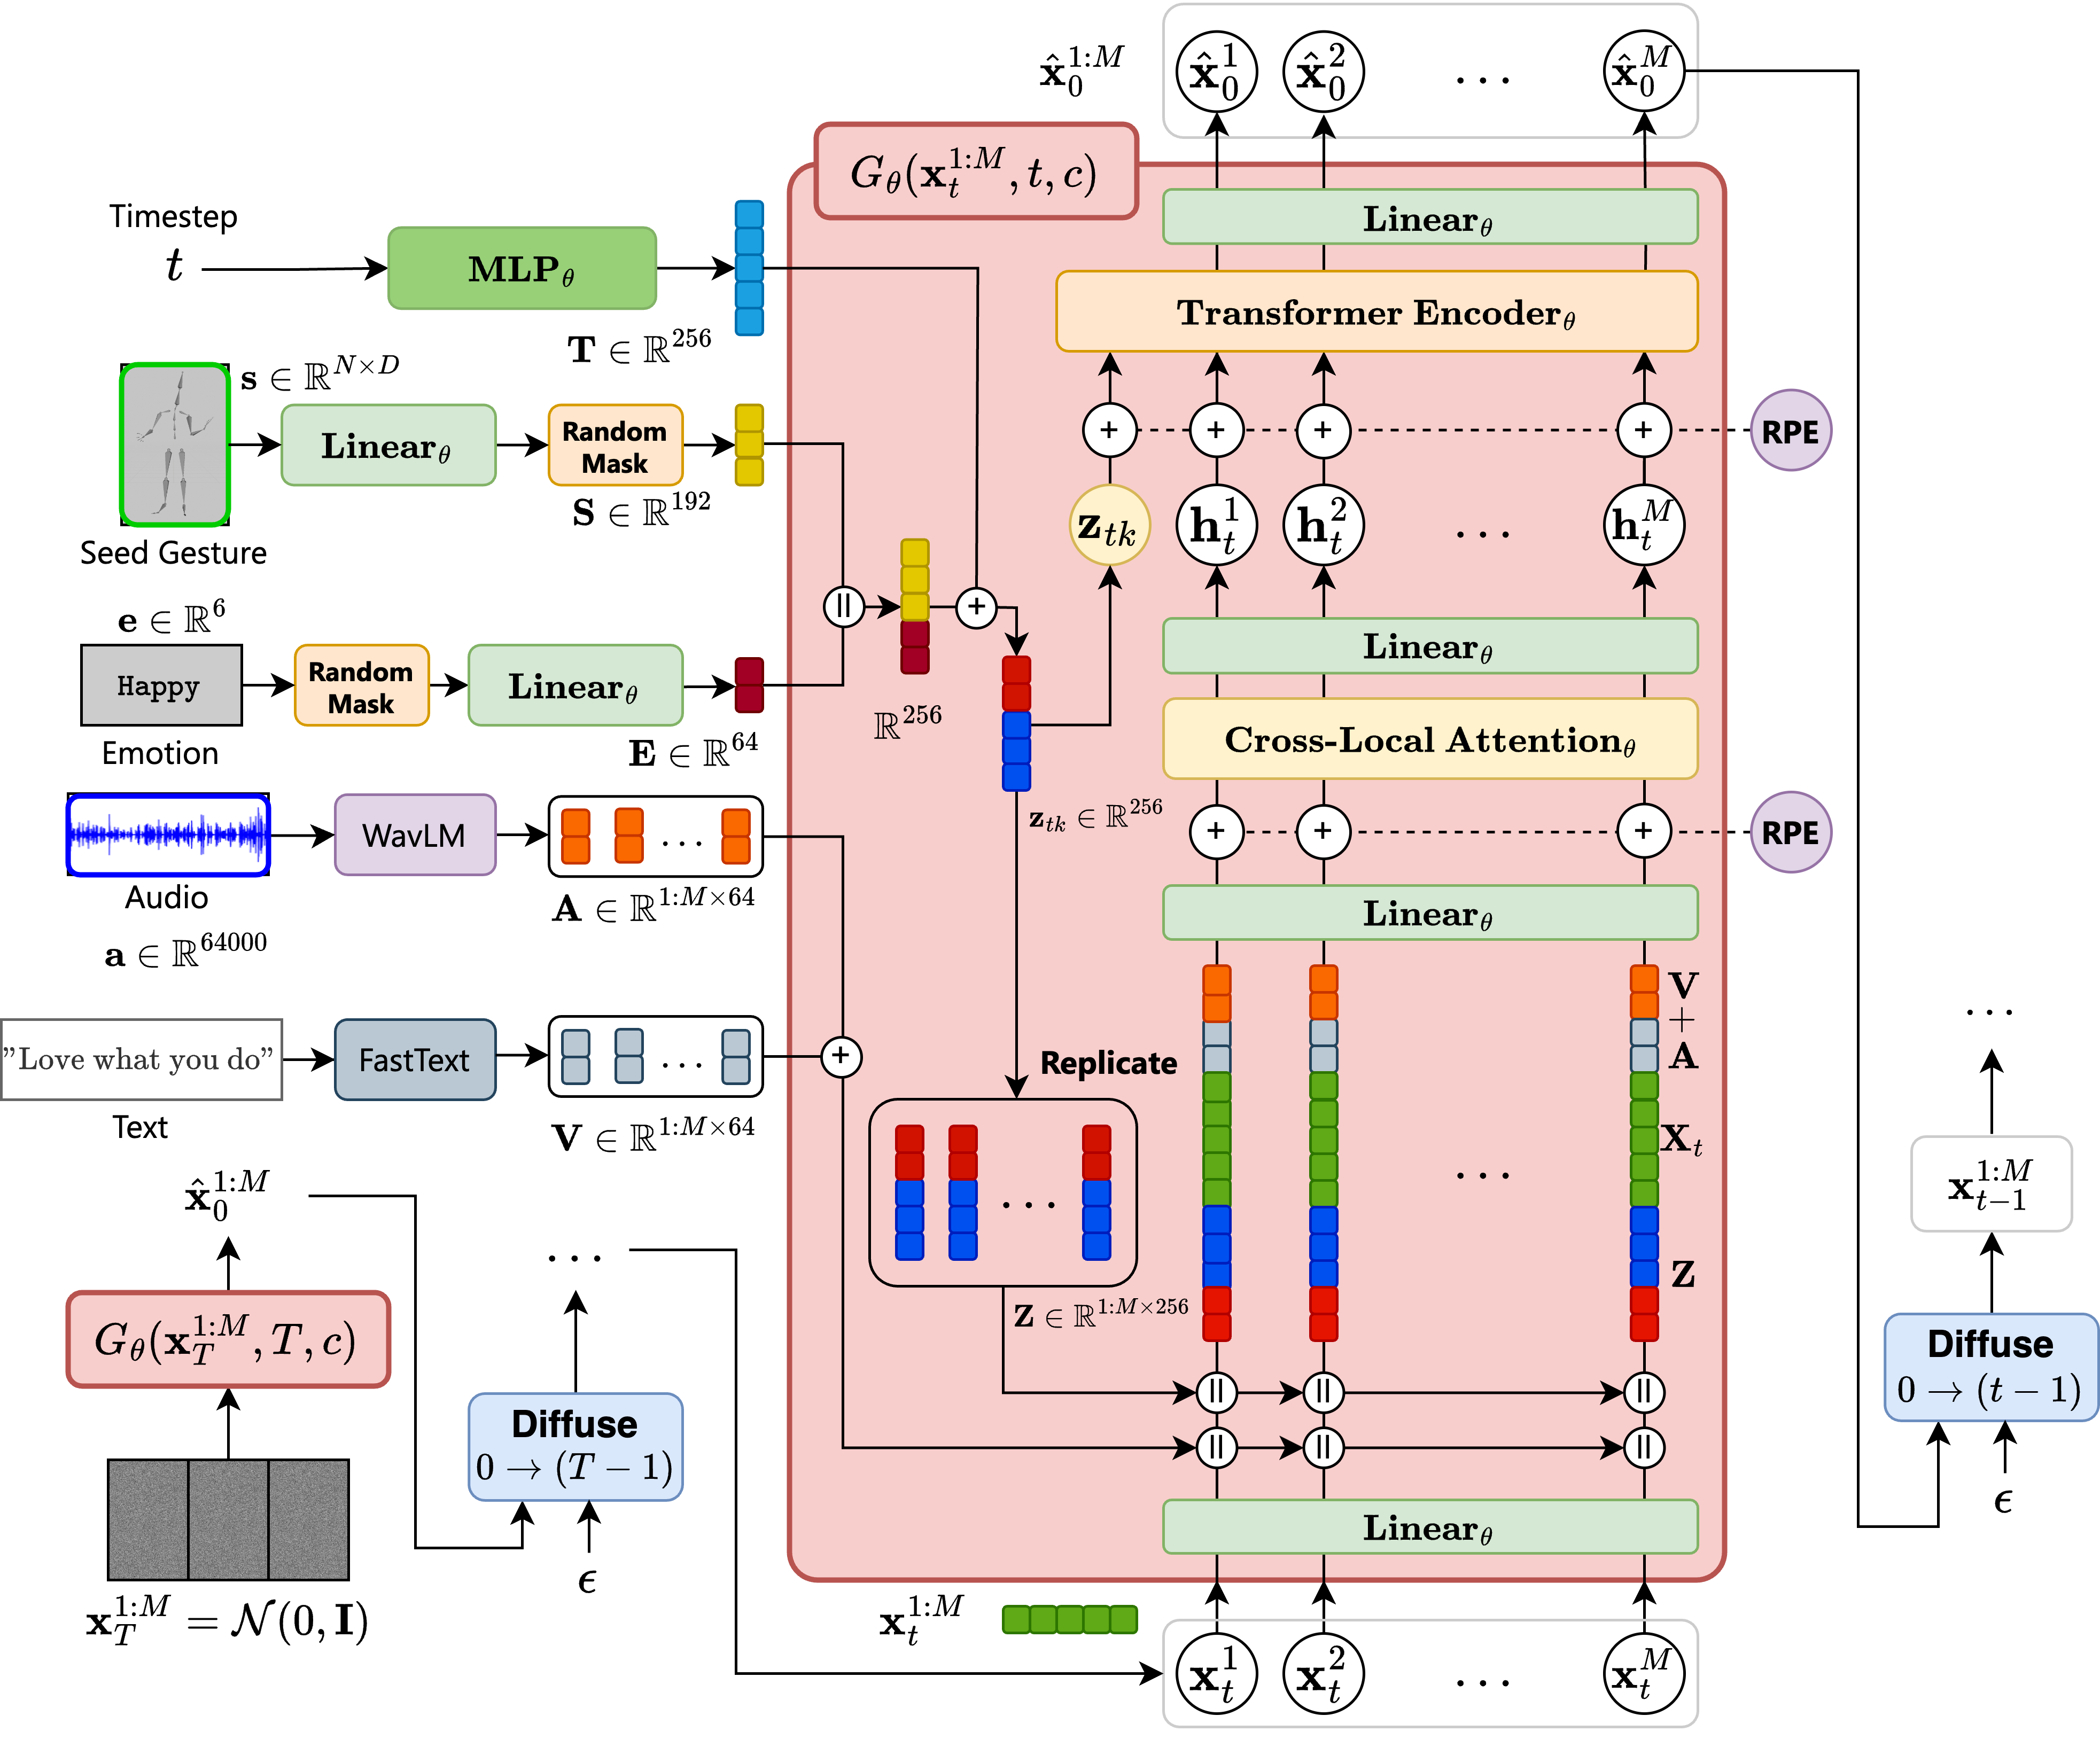
\includegraphics[width=\textwidth]{OHGesture}
	\caption{Mô hình trong OHGesture}
	\label{fig:OHGesture}
\end{figure}
\vspace{-10pt}

\begin{itemize}
	\item \textbf{Bước thời gian $\mathbf{T} \in \mathbb{R}^{256}$ }: Bước thời gian ở mỗi quá trình $t \in [0, T]$, mục tiêu của mô hình là để với bước thời gian $t$ bất kỳ, mô hình có thể tổng quát hoá quá trình khử nhiễu, và có thể học được việc với từng bước $t$ thì giá trị sẽ thay đổi thế nào đối với kết quả dự đoán $\bx_0$. Giá trị timestep $t$ được khởi tạo bằng việc mã hoá nhúng vị trí (Position Embedding) bằng hàm sinusoidal $\text{PE}(t) = \left[ \sin{\left(\frac{t}{10000^{2i / d}}\right)}, \cos{\left(\frac{t}{10000^{2i / d}}\right)} \right]$, sau đó được đưa vào một MLP (Multilayer perceptron) để biến đổi thành vector $\mathbf{T}  \in \mathbb{R}^{256}$.
	
	\item \textbf{Cử chỉ khởi tạo $\mathbf{S} \in \mathbb{R}^{192}$}: Cử chỉ khởi tạo (seed gesture) $\mathbf{s} \in \mathbb{R}^{1:N \times D}$ có được từ cử chỉ ground truth $
	\mathbf{g} \in \mathbb{R}^{(N+M) \times D}$, với mỗi frame là dữ liệu bao gồm $75$ khớp xương, được xử lý theo công thức \ref{eq:gesturevector} để được vector $1141$ chiều, trình bày ở công thức \ref{eq:gesturevector}. Chúng tôi cắt $N = 8$ frame đầu để làm cử chỉ khởi tạo $\mathbf{s}$ và $M = 80$ (4 giây với $20fps$) frame tiếp theo là nhãn để thực hiện quá trình khử nhiễu $\mathbf{x}^{1:M}$. Vector $\mathbf{s}$ đi qua một lớp tuyến tính để được vector $\mathbf{S} \in \mathbb{R}^{192}$, vector $\mathbf{S}$ sau đó được Random Mask trong quá trình huấn luyện để bỏ trong trường hợp nếu một trong $N$ bị thiếu thì sẽ ảnh hưởng như thế nào đến cử chỉ dự đoán.
%	Quá trình này được minh hoạ ở hình \ref{fig:GestureSeries}.
	
%	\item\textbf{Âm thanh}: Âm thanh sẽ được dùng làm đặc trưng để sinh cử chỉ, Chúng tôi sử dụng các mô hình Pretrain có sẵn như WavLM \cite{chen2022wavlm} để trích xuất đặc trưng âm thanh. 
%	Chúng tôi kết hợp thêm các đặc trưng về MFCC, Mel-Spectrum, Pitch, Enery và Onsets \cite{bello2005tutorial}
  \item \textbf{Âm thanh $\mathbf{A} \in \mathbb{R}^{1:M \times 64}$}: Tất cả dữ liệu âm thanh được giảm số sample rate (down sampled) xuống $16 \mathrm{kHz}$, và âm thanh sẽ được lấy tương ứng với cử chỉ là 4s để được vector $\mathbf{a} \in \mathbb{R}^{64000}$, chúng tôi sử dụng mô hình pre-train của WavLM Large \cite{chen2022wavlm} nhúng waveform thô vào  để được vector tiềm ẩn. Sau đó sử dụng nội suy tuyến tính (interpolation) để căn chỉnh đặc trưng của vector tiềm ẩn trong WavLM theo chiều thời gian thành $20fps$, sau đó sử dụng một lớp tuyến tính để giảm kích thước của đặc trưng xuống còn vector đặc trưng với $64$ để tạo thành ma trận cuối cùng $\mathbf{A} \in \mathbb{R}^{M \times 64}$.
		
	\item \textbf{Cảm xúc $\mathbf{E} \in \mathbb{R}^{64}$}: Cảm xúc (emotion) $\mathbf{e} \in \mathbb{R}^{6}$ bao gồm 6 cảm xúc khác nhau được biểu diễn thành một vector theo phương pháp one-hot encoding, sau đó chúng tôi đưa qua một vector tuyến tính để được vector đặc trưng $\mathbf{E} \in \mathbb{R}^{64}$. Mục tiêu là để có thể concat được với vector khởi tạo $\mathbf{S} \in \mathbb{R}^{192} $ để tạo thành vector tiềm ẩn $256$ chiều.
	
	
%	\item \textbf{Cử chỉ nhiễu $\mathbf{x}_{T} \in \mathbb{R}^{M \times D}$} (Noisy gesture): khi huấn luyện, $\mathbf{x}_{t}$ là cử chỉ nhiễu có cùng kích thước như cử chỉ gốc $\mathbf{x}_{0}$ sẽ được sinh ngẫu nhiên từ phân phối chuẩn $\mathcal{N}(0, \mathbf{I})$. Khi sinh ngẫu nhiên, cử chỉ nhiễu ban đầu $\mathbf{x}_{T}$ được lấy mẫu từ phân phối chuẩn chuẩn và các $\mathbf{x}_{t}, t<T$ khác là kết quả của bước làm nhiễu trước đó. Sau đó, kích thước được điều chỉnh thành 256  bằng lớp biến đổi tuyến tính (linear layer).
	\item \textbf{Văn bản $\mathbf{V} \in \mathbb{R}^{1:M \times 300}$}: Văn bản là đoạn văn bản được dịch tương ứng với âm thanh, được đưa vào FastText \cite{bojanowski2017enriching} để thu được một vector có số chiều là 300. Sau đó, được replicate để căn chỉnh tương ứng với $M$ khung hình để được vector đặc trưng $\mathbf{V}$ như hình \ref{fig:OHGesture}.
\end{itemize}

%\item Bước làm nhiễu: Trong quá trình huấn luyện, bước làm nhiễu $t$ được lấy mẫu từ phân phối chuẩn của $\{1,2, \ldots, T\}$, với mã hóa vị trí (position encoding) giống như mô hình Transformer \cite{vaswani2017attention}, sau đó được ánh xạ vào không gian $\mathbf{T}$ có kích thước 256 bằng một mạng perceptron nhiều lớp (MLP).
%
%
%
%\item Cảm xúc: Các cảm xúc của cử chỉ được biểu diễn dưới dạng vectơ one-hot encoding, tức thành vector toàn bộ là số $0$ và vị trí có cảm xúc tương ứng có vị trí là $1$, vector one-hot encoding được ánh xạ vào không gian có kích thước 64 $\mathbf{S}$ thông qua một lớp tuyến tính.
%
%\item Cử chỉ khởi tạo: Cử chỉ khởi tạo giúp tạo ra sự chuyển tiếp mượt mà giữa các lần sinh liên tiếp \cite{yoon2020speech}. Cử chỉ khởi được cắt ngắn xuống $g \in$ $\mathbb{R}^{(8+N) \times 1141}$. Trong quá trình training, $8$ frame đầu tiên của cử chỉ $g$ được sử dụng làm cử chỉ khởi tạo $d$ và $N$ frame còn lại được sử dụng làm cử chỉ thật $x_{0}$ để tính hàm loss $\mathcal{L}$. Sau đó, chúng tôi ánh xạ các đặc trưng của cử chỉ khởi tạo $d$ vào không gian $\mathbf{D}$ có kích thước $192$ chiều bằng một lớp tuyến tính. 
%Kết quả cử chỉ được sinh ra trong $4$ giây, và vì cử chỉ sinh ra được chạy ở $20 \mathrm{fps}$ (tương đương 20 khung hình mỗi giây) nên kích thước $N=80$.

%\section{Mô hình diffusion cho bài toán sinh cử chỉ}
%\vspace{-20pt}
%\begin{figure}
%	\centering
%	\includegraphics[width=0.8\linewidth]{images/OverviewArchitecture.jpg}
%	\vspace{-10pt}
%	\caption{Kiến trúc OHGesture với $T = 4$}
%	\label{fig:architecturediffusion}
%	\vspace{-10pt}
%\end{figure}


% Ý tưởng của chúng tôi là tạo ra các cử chỉ bằng một mô hình diffusion \cite{ho2020denoising} bằng cách học cách dần dần Denoise từ nhiễu hoàn toàn. Như được thể hiện trong Hình 2, mô hình diffusion bao gồm hai phần: quá trình tiến lùi (quá trình diffusion)  và quá trình ngược lại (quá trình Denoise).

%\subsection{Quá Trình Gây Nhiễu (Diffusion)}
%
%Quá trình diffusion $q$ được mô hình hóa như là một quá trình Markov với đầu vào lần lượt được thêm nhiễu, và sau đó mô hình lần lượt từng bước học để có thể tái tạo lại cử chỉ ban đầu.
%Trong bài toán sinh cử chỉ, đầu vào là các điểm trên tọa độ 3D, gọi là keypoint $x$, với $x_{0} \sim q\left(x_{0}\right)$ và $q\left(x_{0}\right)$ là phân phối của dữ liệu thực tế.
%Trong đó mỗi bước phương sai được thay đổi theo hệ số $\beta_{1}, \beta_{2}, \ldots, \beta_{T}$ $\left(0<\beta_{1}<\beta_{2}<\cdots<\beta_{T}<1, T\right)$, chúng tôi thêm nhiễu Gaussian
%
%\begin{equation} \label{eq:gaussian}
%q\left(x_{t} \mid x_{t-1}\right)=\mathcal{N}\left(x_{t} ; \sqrt{1-\beta_{t}} x_{t-1}, \beta_{t} \mathbf{I}\right)
%\end{equation}
%
%vào cử chỉ tại mỗi thời điểm $t$ lần lượt, và sau khi nhiễu Guassian được thêm vào đến bước $T$ đủ lớn, đến khi kết quả trở nên nhiễu hoàn toàn và không thể phân biệt được với kết quả ban đầu.

%\subsection{Quá Trình Khử Nhiễu (Denoise)}
%
%Quá trình Denoise $p_{\theta}$ là quá trình học tham số $\theta$ thông qua một mạng neural. Giả sử quá trình Denoise cũng tuân theo phân phối Gaussian, tức là nhiễu $x_{t}$ tại thời điểm $t$ được sử dụng để học $\mu_{\theta}, \Sigma_{\theta}$, sau đó
%
%\begin{equation} \label{eq:diffusion}
%p_{\theta}\left(x_{t-1} \mid x_{t}\right)=\mathcal{N}\left(x_{t-1} ; \mu_{\theta}\left(x_{t}, t\right), \Sigma_{\theta}\left(x_{t}, t\right)\right)
%\end{equation}
%
%Để thuận tiện cho việc tính toán, ta cho $\alpha_{t}=1-\beta_{t}$ và viết gọn lại $\bar{\alpha}_{t}=\prod_{i=1}^{T} \alpha_{i}$. Sau đó, cử chỉ nhiễu $x_{t}$ tại thời điểm $t$ có thể được viết lại như sau:
%
%\begin{equation} \label{eq:denoisevariance}
%q\left(x_{t} \mid x_{0}\right)=\mathcal{N}\left(x_{t} ; \sqrt{\bar{\alpha}_{t}} x_{0},\left(1-\bar{\alpha}_{t}\right) \mathbf{I}\right)
%\end{equation}
%
%Mô hình học bằng cách tối ưu hóa bằng cách giảm thiểu sự khác biệt giữa nhiễu thực sự $\epsilon$ và nhiễu được dự đoán $\epsilon_{\theta}\left(x_{t}, t\right)$ \cite{ho2020denoising}. Khi lấy mẫu, chúng ta có thể học giá trị trung bình $\mu_{\theta}\left(x_{t}, t\right)=\frac{1}{\sqrt{\alpha_{t}}}\left(x_{t}-\frac{\beta_{t}}{\sqrt{1-\bar{\alpha}_{t}}} \epsilon_{\theta}\left(x_{t}, t\right)\right)$ với phương sai cố định.

%\subsection{Sinh cử chỉ với điều kiện}
%
%Để tổng hợp $M$ frame cử chỉ  $\bx^{1: M}$  với điều kiện $c$ bao gồm cả cử chỉ khởi tạo, văn bản và âm thanh.
%Tương tự như phương pháp \cite{ramesh2022hierarchical} \cite{tevet2022human}, chúng tôi dự đoán dữ liệu thật $\mathbf{x}_0$ thay vì dự đoán nhiễu $\epsilon_{\theta}\left(x_{t}, t\right)$ như  mô hình diffusion cơ bản \cite{ho2020denoising}. Quá trình khử nhiễu (Denoise) tái tạo dữ liệu gốc $\mathbf{x}_{0}$ dựa trên nhiễu đầu vào $\mathbf{x}_{t}$, bước làm nhiễu $t$ và điều kiện $c$.
%
%\begin{equation} \label{eq:condition}
%\hat{\bx}_{0} = G \left( \bx_{t}, t, c\right)
%\end{equation}
%
%%Để 
%%Chúng tôi sử dụng phương pháp concat đặc trưng âm thanh và văn bản để . Ngoài ra chúng tôi cũng sử dụng phương pháp 
%
%Sau đó, hàm khử nhiễu có thể được huấn luyện bằng cách tối ưu hóa hàm Huber loss \cite{huber1992robust} giữa các cử chỉ dự đoán $\hat{x}_{0}$ và các cử chỉ thực tế $\bx_{0}$ trên các tập huấn luyện:
%
%\begin{equation} \label{eq:huberloss}
%\mathcal{L}=E_{x_{0} \sim q\left(x_{0} \mid c\right), t \sim[1, T]}\left[\operatorname{HuberLoss}\left(\bx_{0}-\hat{\bx}_{0}\right)\right]
%\end{equation}




\subsection{Áp dụng cơ chế Attention cho bài toán sinh cử chỉ}

%\subsection{Hàm xử lý đặc trưng của quá trình khử nhiễu}
%
%Như kiến trúc \textbf{OHGesture} trình bày trong hình \autoref{fig:architecturediffusion}, cử chỉ được tạo ra dựa trên bước làm nhiễu $t$, cử chỉ nhiễu $x_{t}$ và điều kiện $c$ (bao gồm âm thanh $a$, cảm xúc $s$ và cử chỉ khởi tạo $d$ ). Đối với mỗi đặc trưng, quá trình sinh cử chỉ được xử lý như sau:


%\subsection{Cơ chế Attention trong hàm khử nhiễu}

Mục tiêu của việc áp dụng cơ chế attention trong mô hình của chúng tôi là mô hình có thể hiểu được mối liên hệ của từng khung hình với nhau, vì vậy phương pháp của chúng tôi là biểu diễn các đặc trưng của từng khung hình bằng các vector đặc trưng riêng lẻ, và với từng đặc trưng của khung hình riêng lẻ, chúng tôi mong muốn tìm được sự tương quan và mối quan hệ giữa các đặc trưng với nhau.
Như hình minh hoạ \ref{fig:OHGesture}, sau quá trình trích xuất đặc trưng. Để tính được sự tương quan của các đặc trưng xa, chúng tôi sẽ học để biểu diễn được các ngữ cảnh cực bộ (local context) theo \cite{rae2020transformers}.


% mà chúng tôi chọn trong mô hình diffusion
Đầu tiên cử chỉ khởi tạo $\mathbf{S}$ và vector cảm xúc $\mathbf{E}$ được ghép lại với nhau để tạo thành một vectơ có kích thước $256$, bởi vì kích thước $256$ là kích thước vector tiềm ẩn. Sau đó được cộng thêm vector timestep $\mathbf{T}$ để tạo thành vector $\mathbf{Z}$. Vector $\mathbf{Z}$ thể hiện thông tin chúng tôi thực sự muốn điều khiển bằng diffusion có điều kiện.

Để có thể căn chỉnh văn bản, âm thanh tương đồng với từng khung hình cử chỉ, chúng tôi sẽ concat các đặc trưng âm thanh, văn bản và cử chỉ đồng thời với nhau. Sau đó để căn chỉnh theo miền thời gian các đặc trưng về cảm xúc và cử chỉ khởi tạo chúng tôi sẽ copy vector $\mathbf{Z}$ để các bản sao của nó được ghép thành một chuỗi vector đặc trưng tương đồng với $M$ khung hình. Sau đó đưa vào lớp local attention (chú ý cục bộ). Tương tự ý tưởng từ phương pháp Routing Transformer \cite{roy2021efficient}, local attention cho thấy rằng sự quan trọng trong việc xây dựng biểu diễn các vector đặc trưng trung gian. Các vector đặc trưng sẽ được cộng thêm một vector sinusoids hay mã hoá vị trí tương đối (Relative position encoding \cite{vaswani2017attention}) để thể hiện được đặc trưng thời gian trước khi đi qua lớp Cross-Local Attention
%mà cho thấy rằng 

%Sau đó, vectơ $\mathbf{Z}$ và các bản sao của nó được ghép thành một chuỗi vector đặc trưng để khớp với dòng thời gian của âm thanh và đặc trưng cử chỉ, sau đó ghép với âm thanh $\mathbf{A}$ và cử chỉ $\mathbf{G}$ để làm đầu vào cho 
%Phương pháp sinh cử chỉ song hành với âm thanh của chúng tôi sử dụng lớp Local Attention được lấy ý tưởng từ 

\begin{equation} \label{eq:attention}
	\operatorname{Attention}(\mathbf{Q}, \mathbf{K}, \mathbf{V}, \mathbf{M})=\operatorname{softmax}\left(\frac{\mathbf{Q} \mathbf{K}^{T}+\mathbf{M}}{\sqrt{C}}\right) \mathbf{V}
\end{equation}

Công thức Attention trên có $\mathbf{Q}$, $\mathbf{K}$ ,$\mathbf{V}$ là các ma trận sau khi đi qua các ma trận biến đối tuyến tính $\mathbf{Q} = \mathbf{X} \mathbf{W}_Q$, $\mathbf{K} = \mathbf{X} \mathbf{W}_K$, $\mathbf{V} = \mathbf{X} \mathbf{W}_V$. Với đầu vào là ma trận biểu thị chuỗi $M$ khung hình, với mỗi khung hình là một vector được concat từ các vector đặc trưng bao gồm cả cử chỉ khởi tạo, văn bản, âm thanh, cảm xúc và cử chỉ $\bx_t$ mà chúng tôi muốn thực hiện khử nhiễu. Quá trình Local-Cross Attention được điều khiển chỉ để tính các đặc trưng cục bộ của chuyển động của các cử chỉ và đặc trưng trong các khung hình lân cận.

Hàm Attention hoạt động như một bộ từ điển, với các thông tin cuối cùng tra được là ma trận $\mathbf{V}$ (value), còn $\mathbf{Q}$ (query) là từ khoá muốn tìm kiếm, $\mathbf{K}$ (key) là danh mục các từ khoá trong bộ từ điển tra cứu. Quá trình Attention sẽ tính toán mức độ tương đồng giữa \( \mathbf{Q} \) và \( \mathbf{K} \) để xác định trọng số cho các giá trị trong \( \mathbf{V} \). Kết quả cuối cùng là tổ hợp các giá trị trong \( \mathbf{V} \), trong đó các giá trị tương ứng với các khoá giống truy vấn nhất sẽ có trọng số cao hơn. $\mathbf{M}$ là mặt nạ (mask) để thực hiện quá trình chú ý cục bộ.

%\begin{equation}
%\begin{aligned}
%	\text{MultiHeadAttn}(\mathbf{X}_q, \mathbf{X}_k, \mathbf{X}_v) &= [\text{head}_1; \dots; \text{head}_h] \mathbf{W}^o \\ 
%	\text{where head}_i &= \text{Attention}(\mathbf{X}_q\mathbf{W}^q_i, \mathbf{X}_k\mathbf{W}^k_i, \mathbf{X}_v\mathbf{W}^v_i)
%\end{aligned}
%\end{equation}


Sau quá trình Cross-Local Attention, mô hình tiếp tục được đưa qua lớp tuyến tính để căn chỉnh tương ứng với $M$ khung hình, bao gồm $\mathbf{h}^{1:M}$.
Sau đó quá trình tương tự như xử lý các vector đặc trưng của mô hình BERT \cite{devlin2019bertpretrainingdeepbidirectional} văn bản. Chúng tôi sử dụng $z$ là $\mathbf{Z} \in \mathbb{R}^{256}$ token đầu tiên biểu thị đặc trưng biểu thị cho toàn bộ chuỗi $M$ khung hình. 
Các vector $\mathbf{h}$ biểu thị cho chuỗi $M$ khung hình, tương tự như phương pháp Reformer \cite{kitaev2020reformer}, trước khi đi vào lớp self-attention trong Transformer Encoder, mô hình sẽ sử dụng lớp mã hoá vị trí tương đối (Relative Position Encoding - RPE) để thay thế mã hoá vị trí tuyệt đối, giúp mô hình hiệu quả hơn trong việc xử lý chuỗi dài.
Khi vào lớp Transformer Encoder \cite{vaswani2017attention} giúp tính toán được mối liên hệ giữa các chuỗi dữ liệu. Trong lớp Transformer Encoder mô hình sẽ áp dụng cơ chế tự chú ý tương tự như trên nhưng không sử dụng mặt nạ. 
%Để yếu tố thời gian không ảnh hưởng nhiều đến kết quả sinh cử chỉ, chúng tôi sử dụng cơ chế mã hóa vị trí tương đối 
Cuối cùng, đầu ra của self-attention được ánh xạ lại cùng kích thước như $\bx_{0}$ sau một lớp biến đổi tuyến tính. Mục tiêu của toàn bộ mô hình $G_\theta ( \mathbf{x}_t, t, c )$ là để học được trọng số $\theta$, với quá trình denoise sẽ giảm dần từ $t = T$ đến khi $t = 1$ ta thu được $\bx_0$.
%Các cơ chế attention khác nhau có thể được tạo ra bằng cách điều chỉnh lớp mask tương ứng $\mathbf{M}$.

%\begin{figure*}[ht]
%\begin{minipage}[b]{0.25\textwidth}
%\centering
%    [width=\textwidth]{images/attention_full.jpg}
%    \caption*{(a) full self-attention}
%\end{minipage}
%\hfill
%\begin{minipage}[b]{0.25\textwidth}
%\centering
%    \includegraphics[width=\textwidth]{images/attention_sidewindow.jpg}
%    \caption*{(b) sliding window attention}
%\end{minipage}
%\hfill
%\begin{minipage}[b]{0.25\textwidth}
%\centering
%    \includegraphics[width=\textwidth]{images/cross_attention.jpg}
%    \caption*{(c) cross-local attention}
%\end{minipage}
%% \label{fig:type_attention}
%\caption[Các loại attention khác nhau (full self-attention, sliding window attention, cross-local attention)]{Các loại attention khác nhau được sử dụng trong các thí nghiệm của chúng tôi, trong đó (a) và (c) là cơ chế attention được sử dụng trong mô hình của chúng tôi và (b) là một mẫu được sử dụng để đánh giá trong thực nghiệm. Mỗi dòng tương ứng với input và mỗi cột tương ứng với output của mô hình}
%\end{figure*}

\begin{figure}[H]
	\centering
	\includegraphics[width=0.6\textwidth]{CrossLocalAttention}
	\caption{Cơ chế Self-Attention trong Transformer Encoder và Cross-Local Attention}
	\label{fig:CrossLocalAttention}
\end{figure}


% Phần 4.3. Các hàng đại diện cho các đầu ra và các cột đại diện cho đầu vào. Các hình vuông màu sáng tô màu cho các phần tử liên quan đến mỗi dòng đầu ra.



%tương tự như phương pháp Longformer \cite{beltagy2020longformer} chúng tôi cũng thử nghiệm cơ chế \textit{sliding window attention}.

%\subsection{Phương pháp sample cử chỉ}


%như kiến trúc trong phần 
%\autoref{fig:architecturediffusion}.


% chúng tôi , trong mỗi bước làm nhiễu $t$, chúng tôi dự đoán cử chỉ sạch  $=$  $\left(x_{t}, t, c\right)$, và thêm nhiễu vào bước làm nhiễu $x_{t-1}$ sử dụng Phương trình (1) với quá trình trải đều. Quá trình này được lặp lại từ $t=T$ cho đến khi đạt được $x_{0}$ (Hình 2 dưới cùng).

\subsection{Điều khiển cảm xúc trong bài toán sinh cử chỉ}

Ở các bước trên mô hình đã có thể học được cách sinh cử chỉ, nhưng để mô hình có thể học được các cảm xúc ở các tình huống khác nhau sẽ được giải quyết bằng cách tham số hóa và lần lượt thay đổi từng cảm xúc để sao cho khi thay đổi cảm xúc thì kết quả dự đoán phải có cảm xúc tương ứng.

Tương tự như các phương pháp sử dụng mô hình khử nhiễu có điều kiện \cite{ho2022classifier}, \cite{tevet2022human}, chúng tôi sử dụng điều kiện $c = [ \mathbf{s}, \mathbf{e}, \mathbf{a}, \mathbf{v} ]$,  bao gồm cử chỉ khởi tạo $\mathbf{s}$, cảm xúc $\mathbf{e}$, âm thanh tương ứng $\mathbf{a}$ và văn bản $\mathbf{v}$. Mô hình diffusion có điều kiện $c$ ở đây sẽ là tổng cả trường hợp ở từng bước $t$ trong mô hình khử nhiễu $\text{G}_\theta \left( \bx_{t}, t, c \right)$, với  $c_{\varnothing}=[\varnothing, \varnothing, \mathbf{a}, \mathbf{v}]$ không điều kiện và $c = [\mathbf{s}, \mathbf{e}, \mathbf{a}, \mathbf{v}]$ có điều kiện. Quá trình này có thể dễ dàng điều khiển bằng một lớp mặt nạ ngẫu nhiên (random mask) trên các vector đặc trưng của cử chỉ khởi tạo $\mathbf{s}$ và cảm xúc $\mathbf{e}$. Khi đó, mô hình chỉ việc thay đổi nhãn tương ứng với lớp mask đã lấy ngẫu nhiên để mô hình có thể tối ưu theo các điều kiện khác nhau. 

%Khi đó hàm khử nhiễu $\text{G}_\theta \left( \bx_{t}, t, c_{1}\right), c_{1}=[\mathbf{s}, \mathbf{e}, \mathbf{a}, \mathbf{v}]$ và hàm khử nhiễu mà không có điều kiện $\text{G}_\theta \left( \bx_{t}, t, c_{2}\right), c_{2}=[\varnothing, \varnothing, \mathbf{a}, \mathbf{v}]$ sẽ được tối ưu trong quá trình huấn luyện, theo công thức

\begin{equation} \label{eq:denoise}
\hat{x}_{0 c, c_{\varnothing}, \gamma}=\gamma G \left(x_{t}, t, c\right)+(1-\gamma) G \left(x_{t}, t, c_{\varnothing}\right)
\end{equation}

Điểm đặc biệt là ta có thể dựa trên việc học có điều kiện và không có điều kiện của classifier-free guidance \cite{ho2022classifier}, ta có thể nội suy giữa hai cảm xúc $\mathbf{e}_1$ và cảm xúc $\mathbf{e}_2$ khác nhau bằng cách cho điều kiện $c = \left[\mathbf{s}, \mathbf{e}_{1}, \mathbf{a}, \mathbf{v} \right]$ và $c_\varnothing = \left[\mathbf{s}, \mathbf{e}_{2}, \mathbf{a}, \mathbf{v} \right]$. Khi đó ta có thể viết lại $\hat{x}_{0 \gamma, c_{1}, c_{2}}=\gamma G \left(x_{t}, t, c_{1} \right)+(1-\gamma) G \left(x_{t}, t, c_{2}\right)$.
%Trong thực tế, hàm Denoise học cả phân phối có điều kiện và không có điều kiện bằng cách ngẫu nhiên phần mask $10 \%$ của các mẫu bằng các mask theo phân phối Bernoulli. Sau đó, đối với kiểu $s$ trong điều kiện, chúng ta có thể tạo ra cử chỉ được kiểm soát kiểu khi lấy mẫu bằng cách nội suy hoặc thậm chí là dự đoán hai biến thể bằng cách sử dụng $\gamma$, như $c_{1}=\left[s, e_{1}, a, v \right], c_{2}=\left[s, e_{2}, a, v \right]$


\subsection{Quá trình huấn luyện}

Thuật toán huấn luyện mô hình OHGesture bắt đầu bằng việc tính toán các giá trị và siêu tham số cần thiết như $\gamma$, $\sqrt{\alpha_t}$, $\sqrt{1 - \alpha_t}$, $\sqrt{\bar{\alpha}_t}$ và nhiễu ngẫu nhiên $\boldsymbol{\epsilon}_t$ cho từng bước thời gian $t$ từ 1 đến $T$. Sau đó, nhãn ban đầu $\mathbf{x}_0$, đại diện cho cử chỉ gốc, được lấy từ phân phối dữ liệu đã chuẩn hóa. Tiếp theo, các mặt nạ Bernoulli $c_1$ và $c_2$ được tạo ngẫu nhiên, mô phỏng các điều kiện khác nhau như cử chỉ, cảm xúc, âm thanh, hoặc văn bản, với một trong các mặt nạ có thể là không có thông tin cảm xúc. Sau khi có các mặt nạ, nhiễu được thêm vào để tạo thành cử chỉ nhiễu $\mathbf{x}_t$, được tính bằng công thức kết hợp chuỗi cử chỉ gốc và nhiễu ngẫu nhiên. Quá trình tiếp theo là chọn ngẫu nhiên một bước thời gian $t$ trong khoảng $[1, T]$ và sử dụng cử chỉ nhiễu $\mathbf{x}_t$ cùng các mặt nạ để dự đoán lại chuỗi cử chỉ gốc thông qua mô hình, trong đó dự đoán được tính bằng một sự kết hợp của các hàm tạo ra từ các điều kiện mặt nạ. Sau khi có dự đoán, loss được tính bằng cách sử dụng HuberLoss giữa chuỗi cử chỉ gốc và dự đoán, từ đó đạo hàm loss để cập nhật các tham số trọng số $\theta$. Quá trình huấn luyện này được lặp lại cho đến khi mô hình hội tụ và thu được các tham số tối ưu $\theta'$.


\begin{algorithm}[H]
	\caption{Thuật toán huấn luyện}
	\setlength{\baselineskip}{10pt}
	\begin{enumerate}
		\item Tính sẵn các giá trị và siêu tham số: $\gamma$, $\sqrt{\alpha_t}$, $\sqrt{1 - \alpha_t}$, $\sqrt{\bar{\alpha}_t}$ và nhiễu ngẫu nhiên $\boldsymbol{\epsilon}_t$ tại mỗi bước $t: 1 \rightarrow T$. Định nghĩa lịch nhiễu $\{\alpha_t \in (0, 1)\}_{t=1}^T$.
		
		\item Lấy nhãn ban đầu $\mathbf{x}_0$ từ phân phối dữ liệu đã chuẩn hóa.
		
		\item Random các mặt nạ Bernoulli $c_{1} = \big[ \mathbf{s}, \mathbf{e_1}, \mathbf{a}, \mathbf{v} \big]$, $c_{2} = \big[ \mathbf{s}, \mathbf{e_2}, \mathbf{a}, \mathbf{v} \big]$, hoặc $c_{2} = \big[ \varnothing, \varnothing, \mathbf{a}, \mathbf{v} \big]$.
		
		\item Thêm nhiễu để có cử chỉ nhiễu $\mathbf{x}_t$:
		\[
		\mathbf{x}_t = \sqrt{\bar{\alpha}_t} \mathbf{x}_0 + \sqrt{1 - \bar{\alpha}_t} \boldsymbol{\epsilon}_t
		\]
		
		\item Với mỗi bước $t$, lấy \textbf{ngẫu nhiên} $t$ từ $[1, T]$.
		
		\item Với $\mathbf{x}_t$, $t$ và các điều kiện mặt nạ $c_1$, $c_2$, dự đoán chuỗi cử chỉ:
		\[
		\hat{\mathbf{x}}_{0 \gamma, c_{1}, c_{2}} = \gamma G_{\theta} \left(\mathbf{x}_{t}, t, c_{1}\right) + (1 - \gamma) G_{\theta} \left(\mathbf{x}_{t}, t, c_{2}\right)
		\]
		
		\item Tính loss và đạo hàm để cập nhật trọng số $\theta$:
		\[
		\mathcal{L}_t = \mathbb{E}_{t \sim [1, T], \mathbf{x}_0, \boldsymbol{\epsilon}_t} \left[ \operatorname{HuberLoss}(\mathbf{x}_0, \hat{\mathbf{x}}_0 ) \right]
		\]
		
		\item Lặp lại từ bước 6 cho đến khi hội tụ, thu được các tham số tối ưu $\theta'$.
	\end{enumerate}
\end{algorithm}

%
%
%\begin{enumerate}
%	\item Tính sẵn các giá trị, và các siêu tham số: $\gamma$, $\sqrt{\alpha_t}$ $\sqrt{1 - \alpha_t}$, $\sqrt{\bar{\alpha}_t}$, Random nhiễu $\bepsilon_t$ ở mọi bước $t: 1 \rightarrow T$.
%	$\{\alpha_t \in (0, 1)\}_{t=1}^T$
%	\item Lấy nhãn $\bx_0$ từ phân bố của dữ liệu đã chuẩn hoá
%	\item Random Bernoulli masks  $c_{1} = \big[ \mathbf{s} , \mathbf{e_1}, \mathbf{a}, \mathbf{v} \big]$, $c_{2} = \big[ \mathbf{s} , \mathbf{e_2}, \mathbf{a}, \mathbf{v}\big]$ hoặc $c_{2} = \big[ \varnothing , \varnothing, \mathbf{a},  \mathbf{v} \big]$
%	\item Forward $\bx_0$ để có cử chỉ nhiễu $\mathbf{x}_t$ :  $\mathbf{x}_t = \sqrt{\bar{\alpha}_t}\mathbf{x}_0 + \sqrt{1 - \bar{\alpha}_t}\boldsymbol{\epsilon}_t$
%	\item $\text{for all}$ $t$, lẫy $t$ \textbf{ngẫu nhiên} $t \sim [1, T]$
%	\item Cho $\bx_t$ và $t$, $c$, $c_{\varnothing}$ để dự đoán chuỗi cử chỉ
%	\begin{equation}
%		\hat{\mathbf{x}}_{0 \gamma, c_{1}, c_{2}}=\gamma G_{\theta} \left(\mathbf{x}_{t}, t, c_{1}\right)+(1-\gamma) G_{\theta} \left(\mathbf{x}_{t}, t, c_{2}\right)
%	\end{equation}
%	\item Tính loss và đạo hàm để cập nhật trọng số $\theta$
%	\begin{equation}
%		\mathcal{L}_t = \mathbb{E}_{t \sim [1, T], \mathbf{x}_0, \boldsymbol{\epsilon}_t} \Big[ \operatorname{HuberLoss}(\mathbf{x}_0, \hat{\mathbf{x}}_0 ) \Big]
%	\end{equation}
%	
%	\item Quay lại bước 6 cho đến khi hội tụ để thu được $\theta'$
%\end{enumerate}


\subsection{Quá trình lấy mẫu}

Để có thể sinh cử chỉ với chiều dài tùy ý, chúng tôi cắt chuỗi ban đầu thành các đoạn ngắn có chiều dài $M$. Trong quá trình huấn luyện, cử chỉ khởi tạo đầu tiên có thể được tạo ra bằng cách lấy ngẫu nhiên cử chỉ từ tập dữ liệu hoặc từ lấy trung bình từ đoạn cắt được. Cụ thể ở đây, sẽ lấy góc quay trung bình trong các đoạn đã cắt được. Tiếp theo chúng ta chỉ việc lấy lần lượt các frame đã sinh ra và chọn $N = 8$ frame cuối cùng làm cử chỉ khởi tạo ở lượt tiếp theo. Đối với mỗi đoạn đã cắt ra, cử chỉ $\bx_{t}$ lần lượt sẽ được áp dụng hàm khử nhiều $\hat{\bx}_{0} = G_{\theta'} \left( \bx_{t}, t, c\right)$, sau khi có $\hat{\bx}_{0}$ ta sẽ Diffuse (thêm nhiễu) cho đến khi được  $\bx_{t-1}$, và $\bx_{t-1}$ sẽ tiếp tục được làm khử nhiễu cho đến bước khử nhiễu $t=1$ sẽ đạt được $\bx_{0}$ 

\begin{algorithm}
	\caption{Thuật toán lấy mẫu (sampling)}
	\setlength{\baselineskip}{10pt}
	\begin{enumerate}
		\item Khởi tạo với nhiễu: $\mathbf{x}_T \sim \mathcal{N}(0, \mathbf{I})$.
		
		\item Các giá trị $\sqrt{\alpha_t}$, $\sqrt{1 - \alpha_t}$ và $\sqrt{\bar{\alpha}_t}$ lấy từ quá trình huấn luyện, tính sẵn giá trị $\sigma_t$ từ $\alpha_t$ ở mỗi bước $t: 1 \rightarrow T$.
		
		\item Chia mỗi đoạn âm thanh 4 giây thành: $\mathbf{a} \in \mathbb{R}^{64000}$. Cử chỉ khởi tạo $\mathbf{s}$ ban đầu là trung bình dữ liệu, sau đó được lấy từ đoạn cử chỉ đã suy luận. Chọn cảm xúc mong muốn, văn bản được lấy từ âm thanh chuyển mã $\mathbf{a}$, tạo cặp điều kiện $c = [\mathbf{s}, \mathbf{e}, \mathbf{a}, \mathbf{v}]$.
		
		\item Với mỗi $t$, lấy $t$ \textbf{tuần tự} từ $[T, \dots, 1]$.
		
		\item Tạo nhiễu ngẫu nhiên $\mathbf{z} \sim \mathcal{N}(0, \mathbf{I})$.
		
		\item Đưa $\mathbf{x}_t$ vào để suy luận $\hat{\mathbf{x}}_0^{(t)} = G_{\theta'}(\mathbf{x}_t, t, c)$.
		
		\item Chuyển tiếp $\hat{\mathbf{x}}_0^{(t)}$ từ bước $0 \rightarrow t$ để nhận $\hat{\mathbf{x}}_{t-1}^{(t)}$.
		
		\item Cộng thêm nhiễu: $\hat{\mathbf{x}}_{t-1} = \hat{\mathbf{x}}_{t-1}^{(t)} + \sigma_t \mathbf{z}$.
		
		\item Quay lại bước 4. Khi $t = 1$, thu được $\hat{\mathbf{x}}_0$ từ quá trình khử nhiễu.
	\end{enumerate}
	\label{alg:sampling}
\end{algorithm}

Thuật toán \ref{alg:sampling} lấy mẫu bắt đầu bằng việc khởi tạo cử chỉ nhiễu ban đầu $\mathbf{x}_T$ từ phân phối chuẩn $\mathcal{N}(0, \mathbf{I})$. Sau đó, các giá trị $\sqrt{\alpha_t}$, $\sqrt{1 - \alpha_t}$ và $\sqrt{\bar{\alpha}_t}$ được lấy từ quá trình huấn luyện, cùng với giá trị $\sigma_t$ được tính từ $\alpha_t$ tại mỗi bước thời gian $t$ từ 1 đến $T$. Mỗi đoạn âm thanh 4 giây được chia thành các chuỗi dữ liệu $\mathbf{a}$, và cử chỉ khởi tạo $\mathbf{s}$ được lấy từ trung bình dữ liệu hoặc từ đoạn cử chỉ đã suy luận. Cảm xúc mong muốn và văn bản được lấy từ âm thanh chuyển mã $\mathbf{a}$, tạo thành một cặp điều kiện $c = [\mathbf{s}, \mathbf{e}, \mathbf{a}, \mathbf{v}]$. Thuật toán sau đó thực hiện các bước tuần tự, bắt đầu từ bước cuối cùng $T$ và tiến ngược về 1. Ở mỗi bước, nhiễu ngẫu nhiên $\mathbf{z}$ được tạo ra và mô hình dự đoán $\hat{\mathbf{x}}_0^{(t)}$ từ cử chỉ nhiễu $\mathbf{x}_t$, thời gian $t$, và cặp điều kiện $c$. Dự đoán này được chuyển tiếp để tính toán $\hat{\mathbf{x}}_{t-1}^{(t)}$ cho bước tiếp theo, và nhiễu được cộng vào để cập nhật cử chỉ tại bước $t-1$. Quá trình này lặp lại cho đến khi đạt đến bước 1, khi đó thuật toán thu được cử chỉ khử nhiễu $\hat{\mathbf{x}}_0$ là kết quả dự đoán cuối cùng.


%\begin{enumerate}
%	\item Bắt đầu với nhiễu: $\bx_T \sim \mathcal{N}(0, \mathbf{I})$
%	\item Các giá trị $\sqrt{\alpha_t}$ $\sqrt{1 - \alpha_t}$ và $\sqrt{\bar{\alpha}_t}$ có được từ bước huấn luyện, tính sẵn các giá trị  $\sigma_t$ từ $\alpha_t$ ở mọi bước $t: 1 \rightarrow T$
%	\item Cắt mỗi 4s âm thanh thành: $\mathbf{a} \in \mathbb{R}^{64000}$, cử chỉ khởi tạo $\mathbf{s}$ ban đầu là trung bình dữ liệu, sau đó được lấy từ đoạn cử chỉ đã suy luận. Chọn cảm xúc mong muốn, văn bản được lấy từ transribe speech $\mathbf{a}$ và tạo cặp condition $c = [\mathbf{s}, \mathbf{e}, \mathbf{a},  \mathbf{v}]$
%	\item $\text{for all}$ $t$, lấy $t$ \textbf{tuần tự} $t \sim [T, \dots 1]$
%	\item Random nhiễu $\bz \sim \mathcal{N}(0, \mathbf{I})$
%	\item Đưa $\bx_t$ vào để suy luận $\hat{\bx}_0^{(t)} = G_{\theta'}(\bx_t, t, c)$
%	\item Forward $\hat{\bx}_0^{(t)}$ $0 \rightarrow t$ để được $\hat{\bx}_{t-1}^{(t)}$
%	\item Cộng thêm một lượng nhiễu $\hat{\bx}_{t-1} = \hat{\bx}_{t-1}^{(t)} + \sigma_t \bz$
%	\item Quay lại bước $4$, khi $t=1$ ta thu được $\hat{\bx}_0$ từ quá trình khử nhiễu
%\end{enumerate}

% \begin{figure*}[ht]
% \begin{minipage}[b]{0.3\textwidth}
% \centering
%     \includegraphics[width=\textwidth]{images/humanlike_score.jpg}
%     \caption*{(a) Biểu đồ hộp của đánh giá về tính giống với con người}
% \end{minipage}
% \hfill
% \begin{minipage}[b]{0.3\textwidth}
% \centering
%     \includegraphics[width=\textwidth]{images/speech_score.jpg}
%     \caption*{(b) Biểu đồ hộp của đánh giá về tính phù hợp giữa cử chỉ và âm thanh.}
% \end{minipage}
% \hfill
% \begin{minipage}[b]{0.3\textwidth}
% \centering
%     \includegraphics[width=\textwidth]{images/style_score.jpg}
%     \caption*{(c) Biểu đồ hộp của đánh giá về tính phù hợp giữa cử chỉ và cảm xúc}
% \end{minipage}
% \label{fig:gesture_score}
% \caption{Biểu đồ hộp mô tả kết quả so sánh MOS cho các mô hình khác nhau trong các chiều khác nhau. Hộp mở rộng từ phân vị thứ nhất thấp nhất (Q1) đến phân vị thứ ba lớn nhất (Q3) của dữ liệu. Đường đỏ chỉ là giữa. Các khe nhỏ biểu thị khoảng tin cậy $95\%$ (CI) xung quanh giữa. Khi CI nhỏ hơn Q1 hoặc lớn hơn Q3, khe mở rộng ra khỏi hộp, tạo ra một hình dáng "lật" độc đáo. Chúng tôi cũng đã đánh dấu giá trị trung bình và khoảng tin cậy $95\%$ của nó trong hình với đường nét đứt màu xanh lá cây và đường dọc màu xanh lam, tương ứng.}
% \end{figure*}


% Hình 4: Biểu đồ hộp thể hiện kết quả so sánh của MOS cho các mô hình khác nhau trong các chiều không gian khác nhau. Hộp mở rộng từ phần tư dưới thứ nhất (Q1) đến phần tư lớn thứ ba (Q3) của dữ liệu. Đường đỏ chỉ ra trung vị. Các rãnh biểu thị khoảng tin cậy $95 \%$ (CI) xung quanh trung vị. Khi CI ít hơn Q1 hoặc lớn hơn Q3, rãnh mở rộng ra ngoài hộp, tạo cho nó một diện mạo "lật" độc đáo. Chúng tôi cũng đã đánh dấu giá trị trung bình và CI $95\%$ của nó trong hình với một đường kẻ xanh lá cây đứt và một đường kẻ đứt màu xanh dương, tương ứng.

% \begin{equation}
% \left[\mathbf{r}_p, \mathbf{r}_r, \dot{\mathbf{r}}_p, \dot{\mathbf{r}}_r, \rho_p, \rho_r, \dot{\rho}_p, \dot{\rho}_r, g_d\right]
% \end{equation}


% Mô hình OHGesture được dựa trên mô hình QPGesture \cite{yang2023qpgesture} với nền tảng chính của phương pháp dựa trên mô hình VQ-VAE là mã hóa (encode) và giải mã (decode) dữ liệu hay nói cách khác chúng ta sẽ biểu diễn toàn bộ dữ liệu ở chiều dữ liệu thấp hơn và sau đó biểu diễn ngược trở lại kích thước ban đầu. Dữ liệu được biểu diễn thành các vùng trong không gian, với mỗi vùng có một đại diện tương ứng. Từ các địa diện ta có thể mã hóa ngược trở lại để chọn ra các ứng viên cử chỉ theo ngữ nghĩa (dữ liệu văn bản) hoặc nhịp điệu lời nói (dữ liệu âm thanh).
% Dựa trên hai cử chỉ ứng viên (gesture candidate), ta trích xuất ra pha dựa trên vận tốc xoay của các các khớp khi di chuyển và dựa trên pha hiện tại của cử chỉ khởi tạo, ta sẽ chọn được cử chỉ có pha gần nhât hay phù hợp nhất để chọn ra chuỗi cử chỉ cuối cùng.

% Cụ thể quá trình huấn luyện của mô hình bao gồm các quá trình như sau: Lượng tử hóa (Quantization), Ghép các chuyển động cử chỉ (Motion Matching), Điều hướng dựa theo pha của cử chỉ (Phrase Guided).

% Kiến trúc mô hình được trình bày minh họa trong hình \autoref{fig:architecturediffusion}.








% \subsection{Lượng tử hóa (Quantization)}
% % Learning a discrete latent space representation

% Lượng tử hóa là việc học để biểu diễn dữ liệu trong không gian rời rạc (discrete latent space representation). Ta sẽ biểu diễn dữ liệu lên không gian tiềm ần (latent space).
% Mục tiêu của việc lượng tử hóa là biểu diễn dữ liệu dưới số chiều thấp hơn hay chấm điểm/đánh giá dựa trên các đặc trưng của dữ liệu, từ đó dùng các điểm đã đánh giá để so sánh với nhau. Sau khi so sánh đánh giá, ta chọn được một ứng viên tốt nhất, từ ứng viên tốt nhất ta sẽ học để giải mã (decode) ngược trở lại dữ liệu ban đầu.

% Dữ liệu đầu vào được lượng tử hóa bao gồm âm thanh, cử chỉ và văn bản. Trong bài toán sinh cử chỉ, chúng tôi chỉ tập trung vào việc xử lý dữ liệu dựa trên cử chỉ nên đôi với dữ liệu văn bản và âm thanh, ta chỉ sử dụng lại các mô hình pre-train có sẵn. Với âm thanh chúng tôi sử dụng mô hình VQ-Wave2Vec \cite{baevski2019vq} để biểu diễn các dữ liệu âm thanh thành các latent vector. Hàm lượng tử hóa âm thanh là hàm $f_{quant\_audio} : \mathbf{A} \mapsto \mathbf{Z_{audio}}$ trong đó $\textbf{A}$ là các chuỗi các âm thanh sẽ được mã hóa lên vector lantent $\textbf{Z}$. Với $\textbf{Z_{audio}} \in \mathcal{Z}_a$.

% Đối với văn bản, chúng tôi sử dụng mô hình Sentene BERT \cite{reimers2019sentence} để biểu diễn các dữ liệu văn bản thành các vector tiềm ẩn. Hàm để nhúng các dữ liệu văn bản thành các vector là hàm $f_{embedding\_text} : \mathbf{T} \mapsto \mathbf{Z_{text}}$.

% Với cử chỉ, mô hình dựa trên kiến trúc của mô hình VQ-VAE. Hàm lượng tử hóa cử chỉ là hàm $f_{quant\_gesture} : \mathbf{G} \mapsto \mathbf{Z_{gesture}}$ với $\textbf{G}$ là các vector trong codebook $\mathcal{Z_g}$

% % Sau đó dựa trên các điểm dữ liệu trước đó để tìm được đại diện phù hợp trong các vùng.
% % Dựa trên chuỗi các dữ liệu đại diện ta có thể tìm được chuỗi các pha của cử chỉ và từ đó chọn ra điểm dữ liệu cuối cùng dựa trên pha của văn bản hoặc âm thanh.

% \subsubsection{Hàm lượng tử hóa cử chỉ (Gesture Quantization)}

% Trong $f_{quant\_gesture}$ các điểm dữ liệu được phân tách và gom nhóm thành các vùng khác nhau trong không gian, với một đại diện để biểu diễn cho mỗi vùng được gọi là \textit{code} là một vector $\textbf{z} \in \mathbb{R}$. Tập các vector đại diện cho các vùng được gọi là \textit{codebook} $\mathbf{Z} \in \mathbb{R}^{D_g \times C}$ là một từ điển được biểu thị dưới dạng một ma trận bao gồm tập nhiều codebook, với mỗi code $\textbf{z} \in \mathbb{R}^C$ và $D_g$ là số lượng phần tử của codebook.

% $$
% f_{encoder} : \mathbf{X} \mapsto \mathbf{Z} \quad \quad
% f_{quantize} : \mathbf{Z} \mapsto \hat{\mathbf{Z}} \quad \quad
% f_{decoder} : \hat{\mathbf{Z}} \mapsto \mathbf{C}
% $$

% $$
% \mathcal{L}=\mathcal{L}_{\text {recontruct }}\left(\mathbf{c}, \mathbf{x}\right)+\left\|\operatorname{sg}[\mathbf{z}]-\mathbf{z}_{\mathbf{q}}\right\| +\beta\left\|\mathbf{z}-\operatorname{sg}\left[\mathbf{z}_{\mathbf{q}}\right]\right\|
% $$

% Loss function:
% $$
% \mathcal{L}_{\text {gesture }\left(E_{g}, D_{g}, \mathcal{Z}_{g}\right)}=\mathcal{L}_{\text {rec }}\left(\hat{\mathbf{G}}_{1}, \mathbf{G}\right)+\left\|\operatorname{sg}[\mathbf{g}]-\mathbf{g}_{\mathbf{q}}\right\| +\beta\left\|\mathbf{g}-\operatorname{sg}\left[\mathbf{g}_{\mathbf{q}}\right]\right\|
% $$

% Loss recontruction:

% $$
% \mathcal{L}_{r e c}\left(\hat{\mathbf{G}}_{1}, \mathbf{G}_{1}\right)=\left\|\hat{\mathbf{G}_{1}}-\mathbf{G}_{1}\right\|_{1}+\alpha_{1}\left\|\hat{\mathbf{G}}_{1}{ }^{\prime}-\mathbf{G}_{1}^{\prime}\right\|_{1} +\alpha_{2}\left\|\hat{\mathbf{G}}_{1}{ }^{\prime \prime}-\mathbf{G}_{1}^{\prime \prime}\right\|_{1}
% $$

% \subsubsection{Quantization Audio}


% $
% \mathbf{g}_{\mathbf{q}, i}=\mathcal{Q_g}(\mathbf{g})=\arg \min _{\mathbf{z}_{j} \in \mathcal{Z}_{g}}\left\|\mathbf{g}_{i}-\mathbf{z}_{j}\right\|
% $

% $
% \hat{\mathbf{G}}_{1}=\mathcal{D}_{g}\left(\mathbf{g}_{\mathbf{q}}\right)=\mathcal{D_g}\left(\mathcal{Q_g}\left(\mathcal{E_g}(\mathbf{G})\right)\right)
% $

% $
% \mathcal{L}=\sum_{k=1}^K \mathcal{L}_k^{\text {wav2vec }}+\left(\|\operatorname{sg}(\mathbf{z})-\hat{\mathbf{z}}\|^2+\gamma\|\mathbf{z}-\operatorname{sg}(\hat{\mathbf{z}})\|^2\right)
% $

% $
% \mathcal{L}_k^{\text {wav2vec }}=-\sum_{i=1}^{T-k}\left(\log \sigma\left(\mathbf{z}_{i+k}^{\top} h_k\left(\mathbf{c}_i\right)\right)+\underset{\tilde{\mathbf{z}} \sim p_n}{\mathbb{E}}\left[\log \sigma\left(-\tilde{\mathbf{z}}^{\top} h_k\left(\mathbf{c}_i\right)\right)\right]\right)
% $


% \section{Motion Matching}
% $
% \hat{\mathbf{C}}_{a}=\left\{\hat{\mathbf{C}}_{a}^{0}, \hat{\mathbf{C}}_{a}^{1}, \ldots, \hat{\mathbf{C}}_{a}^{C_{b}}\right\}
% $

% $
% \hat{\mathbf{C}}_{g}=\left\{\hat{\mathbf{C}}_{g}^{0}, \hat{\mathbf{C}}_{g}^{1}, \ldots, \hat{\mathbf{C}}_{g}^{C_{b}}\right\}
% $

% $
% \hat{\mathbf{C}}_{t}=\left\{\hat{\mathbf{C}}_{t}^{0}, \hat{\mathbf{C}}_{t}^{1}, \ldots, \hat{\mathbf{C}}_{t}^{C_{b}}\right\}
% $



% \subsection{Phrase Guidance}

% \begin{figure}
%     \centering
%     \includegraphics[width=\linewidth]{images/phrase_guidance.png}
%     \caption{Phrase Guidance}
%     \label{fig:PhraseGuidance}
% \end{figure}


% Hàm pha

% $$
% f(\mathcal{T} ; \mathbf{A}, \mathbf{F}, \mathbf{B}, \mathbf{S})=\mathbf{A} \cdot \sin (2 \pi \cdot(\mathbf{F} \cdot \mathcal{T}-\mathrm{S}))+\mathbf{B}
% $$

% Hàm encoder

% $$
% \mathbf{L}=E_{p}(\mathbf{G_{ \text{rotation\_velocity} }})
% $$

% Hàm fourier 
% $$
% \mathbf{c}=F F T(\mathbf{L});\ \ \mathbf{c} \in \mathbb{C}^{M \times K+1}, K=\left|\frac{T}{2}\right|
% $$

% $$
% \mathbf{f}=(0,1 / N, 2 / N, \ldots, K / N)
% $$

% $$
% \mathbf{A}_{i}=\sqrt{\frac{2}{T} \sum_{j=1}^{K} \mathbf{p}_{i, j}}
% $$

% $$
% \quad \mathbf{F}_{i}=\frac{\sum_{j=1}^{K}\left(\mathbf{f}_{j} \cdot \mathbf{p}_{i, j}\right)}{\sum_{j=1}^{K} \mathbf{p}_{i, j}}
% $$


% $$
% \quad \mathbf{B}_{i}=\frac{\mathbf{c}_{i, 0}}{T},
% $$

% Phrase shift
% $$
% \left(s_{x}, s_{y}\right)=F C\left(\mathbf{L}_{i}\right), \quad \mathbf{S}_{i}=\operatorname{atan} 2\left(s_{y}, s_{x}\right)
% $$

% $$
% \mathcal{T}=\left[-\frac{t_{1}-t_{0}}{2},-\frac{t_{1}-t_{0}}{2}+\frac{t_{1}-t_{0}}{N-1}, \ldots, \frac{t_{1}-t_{0}}{2}\right]
% $$


% $$
% \hat{\mathbf{L}}=f(\mathcal{T} ; \mathbf{A}, \mathbf{F}, \mathbf{B}, \mathbf{S})=\mathbf{A} \cdot \sin (2 \pi \cdot(\mathbf{F} \cdot \mathcal{T}-\mathrm{S}))+\mathbf{B}
% $$

% $$
% \hat{\mathbf{G}}_{2}=h(\hat{\mathbf{L}})
% $$

% $$
% \mathcal{P}_{2 i-1}^{(t)}=\mathrm{A}_{i}^{(t)} \cdot \sin \left(2 \pi \cdot \mathrm{S}_{i}^{(t)}\right), \mathcal{P}_{2 i}^{(t)}=\mathrm{A}_{i}^{(t)} \cdot \cos \left(2 \pi \cdot \mathrm{S}_{i}^{(t)}\right)
% $$

% $$
% \mathcal{P} \in \mathbb{R}^{2\ M}
% $$

% $$\mathcal{L}_{\text {phase }}=\mathcal{L}_{\text {phase-recon }}\left(\mathbf{G}, \hat{\mathbf{G}}_{\mathbf{2}}\right)$$




% $$
% \left(
% \left[
%     \hat{
%     \mathcal{P}}_o[-1]^{
%     \left[
%     \left(N_{
%     \text{strid}}-N_{
%     \text{phase}}
% \right):
% \right]}, 
% \mathcal{P}_{a, t}^{
%     \left[N_{
%     \text{strid}}:
% \right]}
% \right]
% \right. 
% , 
% \left.
% \left[
%     \hat{
%     \mathcal{P}}_o[-1]^{
%     \left[-N_{
%     \text{strid}}:
% \right]}, 
% \mathcal{P}_{a, t}^{
%     \left[
%     \left(N_{
%     \text{phase}}-N_{
%     \text{strid}}
% \right):
% \right]}
% \right]
% \right)<
% $$


% $$
% \left(\left[    \hat{    \mathcal{P}}_o[-1]\left[    \left(N_{    \text{strid}}-N_{    \text{phase }}\right):\right], \mathcal{P}_{t, t}^{    \left[        N_{    \text{strid}}:\right]}\right]\right. ,    \left.\left[    \hat{    \mathcal{P}}_o[-1]^{    \left[        -N_{    \text{strid}}:\right]}, \mathcal{P}_{t, t}^{    \left[    \left(N_{    \text{phase }}-N_{    \text{strid}}\right):\right]}\right]\right)
% $$



% $$
% d\left(\operatorname{concat}\left[\hat{\mathcal{P}}_o[-1]\left[\left(N_{\text {strid }}-N_{\text {phase }}\right):\right], \mathcal{P}_{t, t}^{\left[N_{\text {strid }}:\right]}\right]\right. \text {, }   \left.\operatorname{concat}\left[\hat{\mathcal{P}}_o[-1]^{\left[-N_{\text {strid }}:\right]}, \mathcal{P}_{t, t}^{\left[\left(N_{\text {phase }}-N_{\text {strid }}\right):\right]}\right]\right)
% $$

% $$
% d\left(\operatorname{concat}\left[\hat{\mathcal{P}}_o[-1]^{\left[\left(N_{\text {strid }}-N_{\text {phase }}\right):\right]}, \mathcal{P}_{a, t}^{\left[N_{\text {strid }}:\right]}\right]\right. \text {, }   \left.\operatorname{concat}\left[\hat{\mathcal{P}}_o[-1]^{\left[-N_{\text {strid }}:\right]}, \mathcal{P}_{a, t}^{\left[\left(N_{\text {phase }}-N_{\text {strid }}\right):\right]}\right]\right)<
% $$


% $$
% \left[\mathcal{P}_{-1}^{\left[\left(N_{\text {strid }}-N_{\text {phase }}\right):\right]}, \mathcal{P}_{a / t}^{\left[N_{\text {strid }}:\right]}\right]
% $$

% $
% \left[\mathcal{P}_{-1}^{\left[-N_{\text {strid }}:\right]}, \mathcal{P}_{a / t}^{\left[\left(N_{\text {phase }}-N_{\text {strid }}\right):\right]}\right]
% $


\chapter{THỰC NGHIỆM}
\label{Chapter4}

\section{Tập dữ liệu}

\setcounter{figure}{12}
\begin{figure}
	\centering
	\includegraphics[width=\textwidth]{EmotionAnimation}
	\caption{Minh hoạ về 6 cử chỉ $\texttt{Happy}$, $\texttt{Sad}$, $\texttt{Neutral}$, $\texttt{Old}$, $\texttt{Relaxed}$ và $\texttt{Angry}$}
\end{figure}

Luận văn sử dụng tập dữ liệu ZeroEGGS \cite{ghorbani2022zeroeggszeroshotexamplebasedgesture} là một bộ dữ liệu motion capture được xây dựng để nghiên cứu và phát triển các mô hình tạo cử chỉ. Nó bao gồm 67 đoạn độc thoại do diễn viên motion capture nữ thực hiện, với tổng thời gian là 135 phút. Các đoạn hội thoại trong tập dữ liệu được biểu diễn với 6 cảm xúc khác nhau: $\texttt{Happy}$, $\texttt{Sad}$, $\texttt{Neutral}$, $\texttt{Old}$, $\texttt{Relaxed}$ và $\texttt{Angry}$, giúp mô phỏng nhiều trạng thái cảm xúc khác nhau trong cử chỉ và chuyển động cơ thể. ZeroEGGS cung cấp một nền tảng phong phú để nghiên cứu khả năng kết hợp giữa bài nói và cử chỉ động, phục vụ cho việc tạo ra các mô hình có thể điều chỉnh cử chỉ tương ứng với cảm xúc và ngữ nghĩa của văn bản.

\section{Quá trình xử lý dữ liệu}

Dữ liệu luận văn bao gồm các tệp tin BVH (BioVision Motion Capture) được thu nhận từ các cảm biến bằng các hệ thống Motion Capture. 


\textbf{Hierachy}: bao gồm 75 Bone $\{ \mathbf{t}_i \}^{75} $, có vị trí ban đầu  $\mathbf{t}_{i} = \{t_x, t_y, t_z\}$


\vspace{5pt}


\textbf{Motion}:
Bone trong dữ liệu BVH bao gồm vị trí $\mathbf{position}_{\operatorname{local}}  \in \mathbb{R}^{3}$ và góc quay $\mathbf{rotation}_{\operatorname{local}} \in \mathbb{R}^{3}$.

Mô hình của luận văn chuyển dữ liệu từ góc quay Euler sang góc quay Quaternion, với góc quay Quaternion là một véc-tơ gồm 4 phần tử.


\subsection{Tiền xử lý dữ liệu}


Mỗi khung hình chuyển động của một nhân vật hay khung xương (skeleton) bao gồm dữ liệu về toạ độ vị trí và vận tốc theo thời gian.
Ở đây dữ liệu của luận văn của một khung xương với mỗi khung hình (frame) bao gồm:

\begin{equation} \label{eq:gesturevector}
	\mathbf{g} = \Big[ \mathbf{p}_{\text{root}},  \mathbf{r}_{\text{root}},
	\mathbf{ p }'_{\text{root}},  \mathbf{r}'_{\text{root}},
	\mathbf{p}_{\text{joins}},  \mathbf{r}_{\text{joins}},
	\mathbf{p}'_{\text{joins}},  \mathbf{r}'_{\text{joins}},
	\mathbf{d}_{\text{gaze}}
	\Big]
\end{equation}

Trong  đó với mỗi $\mathbf{g} \in \mathbb{R}^{1141}$ bao gồm:
{
	\begin{itemize}
		\item $\mathbf{p}_{\text{root}} \in \mathbb{R}^3$: Toạ độ của điểm gốc
		\item $\mathbf{r}_{\text{root}} \in \mathbb{R}^4$: Góc quay của điểm gốc
		\item $\mathbf{p}'_{\text{root}} \in \mathbb{R}^3$: Vận tốc thay đổi của toạ độ gốc
		\item $\mathbf{r}'_{\text{root}} \in \mathbb{R}^3$: Vận tốc thay đổi của góc quay gốc
		
		\item $\mathbf{p}_{\text{joins}} \in \mathbb{R}^{3 n_{\text{join} }}$: Toạ độ của các khung xương
		\item $\mathbf{r}_{\text{joins}} \in \mathbb{R}^{6 n_{\text{join} }}$: Góc quay của các khung xương theo mặc phẳng X và Y
		\item $\mathbf{p}'_{\text{joins}} \in \mathbb{R}^{3n_{\text{join} }}$: Vận tốc thay đổi của toạ độ các khung xương
		\item $\mathbf{r}'_{\text{joins}} \in \mathbb{R}^{3n_{\text{join} }}$: Vận tốc thay đổi của góc quay các khung xương
		\item $\mathbf{d}_{\text{gaze}} \in \mathbb{R}^3$: Là hướng nhìn
\end{itemize}}


%\begin{figure}
%	\centering
%	\includegraphics[width=0.8\linewidth]{images/skeleton_sample.png}
%	\caption{Minh họa một cử chỉ và mô hình nhân vật}
%	\label{fig:software}
%\end{figure}


Tổng cộng có $75$ khớp (joins) hay $n_{\text{join}} = 75$, với mỗi khung hình (frame) ta sẽ có một vector gồm 1141 chiều.
Tập dữ liệu là tập nhiều chuỗi cử chỉ với độ dài tuỳ ý, từ mỗi cử chỉ độ dài tuỳ tý ta sẽ cắt thành các đoạn $N + M$ khung hình, $g \in \mathbb{R}^{(N + M) \times 1141}$ , trong đó cử chỉ $\mathbf{s} \in \mathbb{R}^{N \times 1141}$ đầu tiên là cử chỉ khởi tạo (seed gesture), $\bx \in \mathbb{R}^{M \times 1141}$ cử chỉ tiếp theo cho việc dự đoán.


Dữ liệu giọng nói $\mathbf{a}_{\text{raw}} \in \mathbb{R}^{ \text{length } }$ là chuỗi giọng nói thô được đọc ở sample rate 16000, sau đó được cắt thành $\mathbf{a} \in \mathbb{R}^{64000}$ tương ứng với 4 giây.
% để  là một chuỗi waveform có độ dài tương ứng với cử chỉ được đọc với sample rate là 16000. 
%\setcounter{figure}{2}

Quá trình này được trình bày ở \autoref{appendix:BVHData:QuaternionConvert}



\section{Quá trình huấn luyện}

Toàn bộ quá trình huấn luyện mô hình được thực hiện trong vòng 1 ngày với các tham số sau: số bước huấn luyện $T = 1000$, sử dụng GPU Nvidia 3090, và chia tập dữ liệu theo tỷ lệ $8:1:1$ cho các tập training, testing và validation. Learning rate được thiết lập là $3 \times 10^{-5}$, với batch size là 384 và tổng cộng 300,000 mẫu. 
$\gamma = 0.1$.

$\beta$ bắt đầu từ $0.5 \rightarrow 0.999$

Quá trình huấn luyện được triển khai trên mã nguồn chương trình có sẵn tại: \hyperlink{https://github.com/hmthanh/OHGesture}{Github/OHGesture} \footnote{\url{https://github.com/hmthanh/OHGesture}}.




\section{Quá trình sử dụng Unity để kết xuất}

Để trực quan hóa quá trình sinh cử chỉ từ dữ liệu đầu ra của mô hình, luận văn sử dụng Unity, kết thừa mã nguồn từ mô hình DeepPhase \cite{starke2022deepphase}  . Dữ liệu sau khi sinh là file BVH (BioVision Motion Capture), trong Unity luận văn bổ sung mã nguồn CSharp để kết xuất theo vị trí toạ độ và nhãn tương ứng, với vị trí và góc quay của các xương được biểu diễn dưới dạng quaternion.

Chi tiết phần render cử chỉ được sinh ra, tôi trình bày ở \autoref{Appendix3}.

Mã nguồn chương trình Unity được luận văn công khai ở \hyperlink{https://github.com/DeepGesture/deepgesture-unity}{Github/DeepGesture-Unity}
\footnote{\url{https://github.com/DeepGesture/deepgesture-unity}}.



\chapter{KẾT QUẢ VÀ ĐÁNH GIÁ}
\label{chap:evalution}

\section{Phương pháp đánh giá}

Quá trình đánh giá được thực hiện qua hai độ đo chính là: Mean Opinion Scores (MOS) và Fréchet Inception Distance (FID).

\subsection{Mean Opinion Scores (MOS)}

Hiện tại, chưa có một độ đo chung cho bài toán sinh cử chỉ, đặc biệt là sinh cử chỉ từ giọng nói, vì vậy luận văn dựa vào đánh giá chủ quan của con người để thực hiện các đánh giá thực nghiệm. 
Tương tự như các phương pháp trước đây \cite{yoon2022genea}; \cite{kucherenko2021large}; các mô hình sinh cử chỉ điều khiển bằng giọng nói vẫn thiếu các chỉ số mục tiêu phản ánh một cách nhất quán với nhận thức chủ quan của con người  \cite{alexanderson2022listen}.
MOS được đo lường thông qua ba tiêu chí:

\begin{itemize}
	\item Human-likeness (Mức độ giống con người)
	\item Gesture-Speech Appropriateness (Sự phù hợp giữa cử chỉ và giọng nói)
	\item Gesture-style Appropriateness (Sự phù hợp giữa phong cách cử chỉ)
\end{itemize}


\subsection{Fréchet Inception Distance (FID)}
FID đo sự tương đồng về phân phối giữa cử chỉ sinh ra $\mathbf{g}$ và cử chỉ thực tế $\mathbf{r}$. Công thức tính FID là:

\begin{equation}
	\text{FID} = \left\| \mu_r - \mu_g \right\|^2 + \operatorname{Tr}\left( \Sigma_r + \Sigma_g - 2 \sqrt{\Sigma_r \Sigma_g} \right)
	\label{eq:fidscore}
\end{equation}


Trong đó:

\begin{itemize}
	\item $\mu$: Trung bình các đặc trưng của cử chỉ.
	\item $\Sigma$: Ma trận hiệp phương sai của đặc trưng.
	\item $\operatorname{Tr}$: Tổng đường chéo chính của ma trận hiệp phương sai.
	\item $\sqrt{\Sigma_r \Sigma_g}$: Sự tương đồng giữa các phân phối cử chỉ thực tế và cử chỉ sinh ra.
\end{itemize}

FID thấp cho thấy phân phối của cử chỉ sinh ra gần giống với cử chỉ thực tế, trong khi FID cao gợi ý sự khác biệt lớn, cho thấy chất lượng cử chỉ sinh ra kém hơn.



\section{Kết quả đánh giá}
\label{sec:result}

\subsection{Kết quả đánh giá bằng MSE}

Trong luận văn, chuỗi cử chỉ dự đoán sẽ được đoạn trên $M$ frame. Luận văn sử dụng Mean Square Error trên chuỗi cử chỉ $\mathbf{x}^{[1:M] \times D}$.

\begin{table}[H]
	\centering
	\resizebox{\textwidth}{!}{%
		\begin{tabular}{lcccccc}
			\hline
			\multicolumn{1}{c}{Cảm xúc} & Tự Nhiên & Buồn Bã &  Vui Vẻ  & Thư Giãn & Lớn Tuổi & Giận Dữ \\ \hline
			DiffuseStyleGesture  & 75.04 & 51.40 & 110.18 & 130.83     & 116.03    & 78.53     \\
			ZeroEGG & 136.33 & 81.22 & 290.47 & 140.24     & 102.44    & 181.07     \\
			\hline
			Mô hình đề xuất                     &         &         &         &           &          &                 \\
			\quad \textbf{OHGesture} & 161.22 & 89.58 & 279.95 & 156.93   & 99.86   & 215.24    \\
			\hline
		\end{tabular}%
	}
	\caption{Kết quả đánh giá Mean Square Error theo 6 cảm xúc}
	\label{table:EvaluationMSE}
\end{table}

\subsection{Kết quả đánh giá bằng MOS}

Ở đây luận văn sử dụng lại kết quả đánh giá của mô hình baseline \textbf{DiffuseStyleGesture} \cite{yang2023diffusestylegesture} trong độ đo về  cảm nhận đánh giá của con người do lĩnh vực sinh cử chỉ vẫn còn rất mới, chi phí để ước lượng các mô hình còn lớn nên luận văn không thể đánh giá được mô hình OHGesture. Vì vậy các kết quả này chưa bao gồm thông tin kết quả về mô hình \textbf{OHGesture} mà luận văn đề xuất.

\begin{figure}[htbp]
	\centering
	\begin{subfigure}[b]{0.3\textwidth}
		\includegraphics[width=\textwidth]{BoxHumanLikeness.pdf}
		\caption*{(a) Human-likeness}
	\end{subfigure}
	\hfill
	\begin{subfigure}[b]{0.3\textwidth}
		\includegraphics[width=\textwidth]{BoxSpeechAppropriateness.pdf}
		\caption*{\small (b) Speech Appropriateness}
	\end{subfigure}
	\hfill
	\begin{subfigure}[b]{0.3\textwidth}
		\includegraphics[width=\textwidth]{BoxStyleAppropriateness.pdf}
		\caption*{(c) Style Appropriateness}
	\end{subfigure}
	
	\label{fig:compare }
\end{figure}


Để hiểu hiệu suất thị giác thực tế của phương pháp của luận văn, luận văn tiến hành một nghiên cứu người dùng so sánh các cử chỉ được tạo ra từ phương pháp của luận văn và dữ liệu chụp chuyển động thực tế. Độ dài của các đoạn clip đánh giá dao động từ 11 đến 51 giây, với độ dài trung bình là 31.6 giây, dài hơn so với các đoạn trong đánh giá GENEA \cite{yoon2022genea} (8-10 giây), vì thời gian dài hơn có thể tạo ra kết quả rõ ràng và thuyết phục hơn \cite{yang2022reprgesture}. Người tham gia đánh giá trên thang điểm từ 5 đến 1, với các nhãn từ $\texttt{excellent}$,  $\texttt{good}$, $\texttt{fair}$, $\texttt{poor}$, đến $\texttt{bad}$. 

\begin{table}[H]
	\centering
	\begin{tabular}{lcc}
		\hline
		\multicolumn{1}{c}{Name} &
		\begin{tabular}[c]{@{}c@{}}Human\\ likeness \end{tabular}$\uparrow$ &
		\begin{tabular}[c]{@{}c@{}}Gesture-speech\\ appropriateness\end{tabular}$\uparrow$ \\ \hline
		Ground Truth          & 4.15 $\pm$ 0.11          & 4.25 $\pm$ 0.09          \\
		Ours                  & \textbf{4.11 $\pm$ 0.08} & \textbf{4.11 $\pm$ 0.10} \\
		\quad$-$ WavLM             & 4.05 $\pm$ 0.10          & 3.91 $\pm$ 0.11          \\
		\quad$-$ Cross-local attention   & 3.76 $\pm$ 0.09          & 3.51 $\pm$ 0.15          \\
		\quad$-$ Self-attention    & 3.55 $\pm$ 0.13          & 3.08 $\pm$ 0.10          \\
		\quad$-$ Attention + GRU&
		3.10 $\pm$ 0.11 &
		2.98 $\pm$ 0.14 \\
		\quad$+$ Forward attention & 3.75 $\pm$ 0.15          & 3.23 $\pm$ 0.24          \\
		\hline
	\end{tabular}
	\caption{Kết quả đánh giá bằng MOS trên Genea (năm 2022)}
	\label{table:MOSScore}
\end{table}
%Kết quả của các nghiên cứu loại bỏ (Ablation studies). "$-$" chỉ các mô-đun không được sử dụng và "$+$" chỉ các mô-đun bổ sung. Chữ in đậm chỉ ra chỉ số tốt nhất

\subsection{Kết quả đánh giá bằng FGD}

Luận văn đề xuất Fréchet Gesture Distance (FGD), hệ số FID dựa trên cử chỉ (gesture), và xây dựng mã nguồn \hyperlink{https://github.com/GestureScore/GestureScore}{GestureScore} \footnote{Github/GestureScore: \url{https://github.com/GestureScore/GestureScore}} . Trong GestureScore, luận văn xây dựng một Inception V3 model, để mã hóa chuỗi khung hình $\bx^{1:M \times D}$ thành vector tiềm ẩn kích thước $32 \times 32$. Sử dụng vector này làm đầu vào cho \autoref{eq:fidscore}. Sau đây là \autoref{table:EvalFGD} đánh giá kết quả của mô hình OHGesture bằng GestureScore

%$\uparrow$
\begin{table}[H]
	\centering
	\begin{tabular}{lcc}
		\hline
		\multicolumn{1}{c}{Name} & FGD trên vector đặc trưng & \begin{tabular}[c]{@{}c@{}} FGD dữ liệu gốc \end{tabular} \\ \hline
		Ground Truth             & -       & -          \\
		Ours                     &       & \\
		\quad OHGesture (Feature D=1141) & 2.058      & 9465.546 \\
		\quad OHGesture (Rotations) & 3.513       & 9519.129 \\
		\hline
		
	\end{tabular}
	\caption{Kết quả đánh giá Fréchet Gesture Distance (FGD) trên $\bx^{1:M \times D}$ (từ frame 1 đến frame M, mỗi frame có D đặc trưng từng khung hình )}
	%	\caption{Kết quả của các nghiên cứu loại bỏ (Ablation studies). "$-$" chỉ các mô-đun không được sử dụng và "$+$" chỉ các mô-đun bổ sung. Chữ in đậm chỉ ra chỉ số tốt nhất.}
		\label{table:EvalFGD}
\end{table}

\begin{itemize}[]
		\item \textbf{Vector đặc trưng}
	Sử dụng tệp BVH để chuyển toàn bộ skeleton của mỗi khung hình thành vector đặc trưng $D = 1141 $ như công thức  \autoref{eq:gesturevector}
	
	\item  \textbf{Rotations}: Từ tệp BVH kết quả, luận văn trích xuất sự thay đổi của các góc quay (rotations), $D = 225$ ($225 = 75 \times 3$) của chuỗi cử chỉ với chiều dài mỗi đoạn là $M$ frame để đánh giá ở dòng OHGesture bên dưới. 
	
\end{itemize}

\section{Xây dựng và tiêu chuẩn hóa hệ thống đánh giá kết quả sinh cử chỉ}

Hiện nay các mô hình sinh (gesture generation) cử chỉ được quan tâm nghiên cứu với rất nhiều mô hình khác nhau, tuy nhiên do không có độ đo chung, vì các độ đo truyền thống như FID (Fréchet Inception Distance) hay IS (Inception Score),.. không thể hiện được hết các tính chất Giống người (Human-likeness), tính phù hợp với giọng nói (Speech Appropriateness), và tính phù hợp với phong cách (Style Appropriateness) của cử chỉ. Các mô hình cũng được thực hiện và huấn luyện trên một tập dữ liệu khác nhau, vì vậy rất khó để biết được mô hình nào đã đạt kết quả tốt hơn, và mô hình nào là mô hình state-of-the-art, từ đó khó có thể đạt được sự tiến bộ trong lĩnh vực sinh cử chỉ. Việc thiếu tiêu chuẩn chung để đánh giá trong cộng đồng nghiên cứu khiến luận văn mong muốn xây dựng một hệ thống xếp hạng trực tuyến \cite{nagy2024towards} \hyperlink{https://genea-workshop.github.io/leaderboard/}{GENEA Leaderboard} \footnote{GENEA Leaderboard: \url{https://genea-workshop.github.io/leaderboard/}}., là một bảng xếp hạng các mô hình sinh cử chỉ. Luận văn thu thập và xử lý một tập dữ liệu cử chỉ từ nhiều ngôn ngữ và từ nhiều tập dữ liệu khác nhau và tiêu chuẩn hóa để tạo ra một tập dữ liệu duy nhất.  Sau đó, luận văn sẽ mời các tác giả của các mô hình để học và dự đoán trên tập dữ liệu đã được tiêu chuẩn hóa, sau khi có kết quả sinh cử chỉ, luận văn sẽ thuê những người tham gia nghiên cứu trên Prolific để đánh giá và xếp hạng kết quả sinh cử chỉ của các mô hình. Hiện tại luận văn đang xây dựng hệ thống trực tuyến \hyperlink{https://github.com/hemvip/hemvip.github.io}{hemvip/hemvip.github.io}\footnote{HEMVIP2 \url{https://github.com/hemvip/hemvip.github.io}} với mục tiêu đánh giá kết quả sinh của cử chỉ thông qua việc thuê các người tham gia đánh giá kết quả thông qua Prolific. Luận văn sẽ bổ sung các đánh giá về mô hình OHGesture dựa trên các điểm số trên.


Thông qua hệ thống đánh giá này, nghiên cứu kỳ vọng sẽ thiết lập một tiêu chuẩn chung, từ đó tạo động lực cho sự tiến bộ trong lĩnh vực sinh cử chỉ.


\input{6_Conclusion/Conclusion.tex}

\input{References/References.tex}
\include{References/Publish}

\appendix
\renewcommand{\chaptername}{Phụ lục}
\chapter{Các tham số}
 \label{Appendix1}

\section{Sự thay đổi của $\sqrt{\alpha}$ và $\sqrt{1 - \alpha}$}

\setcounter{figure}{13}
\begin{figure}
	\includegraphics[width=0.5\linewidth]{SquareAlpha}
	\label{fig:wrapfig}
	\caption{Sự thay đổi của $\sqrt{\alpha}$ và $\sqrt{1 - \alpha}$}
\end{figure}

Trong quá trình diffusion, hệ thống muốn giảm dần sự hiện diện của $\bx$ và tăng dần sự hiện diện của nhiễu $\epsilon_t$. Với $\mathbf{x}_t = \sqrt{\alpha_t} \mathbf{x}_t + \sqrt{1 - \alpha_t} \epsilon_t$. Các hệ số $\sqrt{\alpha_t}$ và $\sqrt{1 - \alpha_t}$ giúp điều khiển quá trình này như sau:



\begin{itemize}
	\item $\sqrt{\alpha_t}$: Ban đầu giá trị lớn nhưng giảm dần để giảm sự ảnh hưởng vào kết quả tổng giữa nhiễu và $\bx_t$
	\item $\sqrt{1 - \alpha_t}$: Ban đầu giá trị nhỏ nhưng tăng dần theo từng bước. Với mục tiêu là đến cuối cùng thì sự ảnh hưởng của nhiễu càng lớn và trở thành nhiễu hoàn toàn.
\end{itemize}


Cả hai đại lượng này thay đổi theo thời gian trong quá trình diffusion, từ đó quyết định mức độ nhiễu được thêm vào từng bước $t$ và mức độ giữ lại trạng thái trước đó qua từng bước.


\section{Sự thay đổi của $\sqrt{\bar{\alpha}}$ và $\sqrt{1 - \bar{\alpha}}$}

$\bar{\alpha}_t = \prod_{i=1}^t \alpha_i$.  $\sqrt{1 - \bar{\alpha}_t} = \sqrt{1 - \prod_{i=1}^t \alpha_i}$. Cả $\sqrt{\bar{\alpha}}$ và $\sqrt{1 - \bar{\alpha}}$ đóng một vai trò quan trọng trong quá trình huấn luyện và sinh cử chỉ. Giúp kiểm soát mức độ nhiễu được thêm vào và cử chỉ, ta có thể thấy $\sqrt{\bar{\alpha}}$ giảm dần còn $\sqrt{1 - \bar{\alpha}}$ thì tăng dần..


\begin{figure}
	\includegraphics[width=\linewidth]{AlphaCumprod}
	\label{fig:AlphaCumprod}
	\caption{Quá trình thay đổi của $\sqrt{\bar{\alpha}}$ và $\sqrt{1 - \bar{\alpha}}$}
\end{figure}



%Praesent in sapien. Lorem ipsum dolor sit amet, consectetuer 
%adipiscing elit. Duis fringilla tristique neque. Sed interdum

%\begin{figure*}[p]
%	\centering
%	\includegraphics[width=0.5\linewidth]{images/beta_sqrtbeta}
%	\caption{Sự thay đổi của $\sqrt{\beta}$ và $\sqrt{1-\beta}$}
%	\label{fig:beta_sqrtbeta}
%\end{figure*}


%You can put more than one value in the parameter, for instance, if you write [ht] LaTeX will try to position the figure here, but if it's not possible (the space may be insufficient) then the figure will appear at the top of the page. It is recommended to use more than one positioning parameter to prevent unexpected results.

\chapter{Quá trình xử lý dữ liệu BVH}
\label{Appendix2}

\section{Cấu trúc tệp dữ liệu BVH}

File BVH (Biovision Hierarchy) là một định dạng file dữ liệu chứa thông tin về cấu trúc xương và dữ liệu về chuyển động của xương trong một hệ thống xương. File BVH bao gồm hai phần chính: phần khai báo cấu trúc xương và phần dữ liệu chuyển động của xương. 
%Mỗi phần được phân cách bởi từ khóa \texttt{MOTION}.

\setcounter{figure}{15}
\begin{figure}
	\centering
	\includegraphics[width=\linewidth]{BVH}
	\caption{Quá trình xử lý tệp tin BVH}
	\label{fig:BVH}
\end{figure}


	\textbf{Hierachy}: bao gồm 75 Bone $\{ \mathbf{t}_i \}^{75} $, có vị trí ban đầu  $\mathbf{t}_{i} = \{t_x, t_y, t_z\}$

\vspace{5pt}

\textbf{Motion}:
Bone trong dữ liệu BVH bao gồm vị trí $\mathbf{position}_{\operatorname{local}}  \in \mathbb{R}^{3}$ và góc quay $\mathbf{rotation}_{\operatorname{local}} \in \mathbb{R}^{3}$.
%	\begin{figure}
	%		\centering
	%		\includegraphics[width=0.25\textwidth]{BVHFile}
	%	\end{figure}
$\mathbf{rotation}_i^{\operatorname{local}} = \{ \alpha ,\beta , \gamma \}$ lần lượt là góc quay quanh các trục $Z$ ,$Y$ , và $X$, góc quay tổng hợp ba trục trong không gian Eule là $R = R_Z(\alpha) R_Y(\beta) R_X(\gamma)$.
Để tính toạ độ chuyển động của một nhân vật, ta thực hiện phép toán sau:

\begin{equation}
	\mathbf{position}_{\text{global}} = R \cdot \mathbf{position}_{\text{local}} + \mathbf{t}
\end{equation}


\section{Quá trình chuyển góc quay Euler sang Quaternion}

%Quaternion là một cách biểu diễn góc quay trong không gian ba chiều. Quaternion có dạng $q = a + bi + cj + dk$, trong đó $ư, b, c, d$ là các số thực. Quaternion có thể được biểu diễn dưới dạng ma trận $4 \times 4$ như sau:


Để tránh Gimbal lock, ta phải chuyển dữ liệu ở dạng góc quay Euler sang dạng góc quay Quaternion. Trong đó góc quay từng Bone dạng Euler ZYX sang dạng Quaternion, mỗi Bone biểu diễn bằng 4 phần tử $q = (q_w, q_x, q_y, q_z)$, với các giá trị được tính như sau:
%	Mỗi Bone được biểu diễn thành: 
%	$$q = w + xi + yj + zk$$
%	c
%	$$i^2 = j^2 = k^2 = ijk = -1$$

Đầu tiên, chúng ta tính các giá trị $\cos$ và $\sin$ của một nửa góc quay cho mỗi trục:


\begin{itemize}
	\item $c_{\alpha} = \cos\left(\frac{\alpha}{2}\right), \quad s_{\alpha} = \sin\left(\frac{\alpha}{2}\right)$
	\item $c_{\beta} = \cos\left(\frac{\beta}{2}\right), \quad s_{\beta} = \sin\left(\frac{\beta}{2}\right)$
	\item $c_{\gamma} = \cos\left(\frac{\gamma}{2}\right), \quad s_{\gamma} = \sin\left(\frac{\gamma}{2}\right)$
\end{itemize}

Dựa trên các giá trị tính được ở trên, các thành phần của quaternion được tính như sau:


\begin{itemize}
	\item $q_w = c_{\alpha} c_{\beta} c_{\gamma} + s_{\alpha} s_{\beta} s_{\gamma}$
	\item $q_x = c_{\alpha} c_{\beta} s_{\gamma} - s_{\alpha} s_{\beta} c_{\gamma}$
	\item $q_y = c_{\alpha} s_{\beta} c_{\gamma} + s_{\alpha} c_{\beta} s_{\gamma}$
	\item $q_z = s_{\alpha} c_{\beta} c_{\gamma} - c_{\alpha} s_{\beta} s_{\gamma}$
\end{itemize}

Với quaternion $q$ đã tính, vị trí toàn cục của bone $\mathbf{p}_{\text{global}}$ được xác định bằng cách quay vị trí cục bộ $\mathbf{p}_{\text{local}}$ thông qua công thức:

\begin{equation}
	\mathbf{p}_{\text{global}} = q \cdot \mathbf{p}_{\text{local}} \cdot q^{-1} + \mathbf{t}
\end{equation}

với $\mathbf{t}$ là vị trí gốc của bone trong không gian toàn cục.




%\include{Appendix/Appendix3}

\end{document}